\documentclass[a4paper,11pt,twoside]{unimelb-thesis_CODBD}%

\NeedsTeXFormat{LaTeX2e}
\usepackage{amsmath,amsfonts,bm}
\usepackage{amsmath}
\usepackage{amssymb}
\usepackage{booktabs}
\usepackage{color}
\usepackage{dcolumn}
\usepackage{graphicx}
\usepackage{epstopdf}
\usepackage{MnSymbol}
\usepackage{mathtools}
\usepackage[round]{natbib}
\usepackage[compact]{titlesec}
\usepackage[acronym]{glossaries} % Used to make a list of abbreviations
\usepackage{longtable}
\usepackage{afterpage}
\usepackage[export]{adjustbox}[2011/08/13]
\usepackage{float}
% Set up geometry and line spacing
% \usepackage[top=0.5in, bottom=0.5in, left=1.0in, right=0.75in, headheight=13.0pt, includeheadfoot]{geometry} % Pinched Crown @ 10pt
\usepackage[top=3.0cm, bottom=2.25cm, left=3.5cm, right=3.0cm, headheight=15.5pt, includeheadfoot]{geometry} % A4 @ 11pt
% \usepackage[top=4cm, bottom=3.0cm, left=3.5cm, right=3.0cm, headheight=15.5pt]{geometry}
\newcommand{\pending}[1]{\textcolor{red}{#1}}
\newcommand{\arcmin}{\ensuremath{^{\prime}}}
\newcommand{\figwidth}{1.0\textwidth}
\newcommand{\bL}{\bm{\ell}}
\newcommand{\am}{$^{\prime}$}
\newcommand{\howmanysigmaforfullsample}{8.7$\sigma$}
\newcommand{\sptpol}{SPTpol}
\newcommand{\sqdeg}{deg$^{2}$}
\newcommand{\ukam}{${\rm \mu K^{\prime}}$ }
\newcommand{\fitAforvlsamplewithsyserrorsformatted}{\ensuremath{2.70 \pm 0.51~{\rm [stat.]} \pm~0.06~{\rm [sys.]}}}
\newcommand{\bnhat}{\bm{\hat{\mbox{n}}}}
\newcommand{\mvir}{M_{200m}}
\newcommand{\RM}{redMaPPer} 
\newcommand{\ML}{\ensuremath{M-\lambda}}
\newcommand{\whichyear}{\mbox{Year-3}}
\newcommand{\whichcatversion}{\texttt{y3\_gold:v6.4.22}}
\newcommand{\tbd}[1]{\textcolor{red}{#1}}
\newcommand{\ukarcmin}{\ensuremath{\mu}{\rm K-arcmin}}
\newcommand{\sr}[1]{\textcolor{red}{[SR: #1]}}
\newcommand{\snr}{$S/N$}
\newcommand{\msol}{\ensuremath{{M}_{\odot}}}
\newcommand{\munits}{\ensuremath{10^{14}~ \msol}}
\newcommand{\howmanyclustersinfullsamplenorichnesscut}{4003}
\newcommand{\howmanyrandomsforMF}{50,000}
\newcommand{\howmanyclustersinfullsample}{4003}
\newcommand{\howmanysigmaforcosmosample}{6.7$\sigma$}
\newcommand{\fitmassforfullsample}{1.28}% $\times$ \munits }
\newcommand{\fitmassforfullsamplewitherrors}{$1.28^{+0.14}_{-0.18}$}% $\times$ \munits }
\newcommand{\fitmassforfullsamplewithsyserrors}{\ensuremath{1.28^{+0.14}_{-0.18} {\rm ~[stat.]} \pm 0.03 ~{\rm [sys.]} }} % $\times$ \munits }
\newcommand{\fitmassforfullsamplewitherrorslgmca}{\pending{ xx}}% $\times$ \munits }
\newcommand{\fitmassforfullsamplewithszfreemaps}{$1.76^{+0.23}_{-0.29}$}% $\times$ \munits }
\usepackage{setspace}
\onehalfspacing
%
% Set up the font to use
\usepackage[T1]{fontenc}
\renewcommand{\encodingdefault}{T1}

% Import custom macros and commands
% Provide the hardcore conditional macros.

% \providecommand{\varname}[3]{{\ensuremath{{#1}_{\scriptscriptstyle #2}^{\scriptscriptstyle #3}}}}
% \providecommand{\subvar}[2]{\varname{#1}{#2}{}}
% \providecommand{\vecvar}[4][\@empty]{\varname{\boldsymbol{#2}}{\ifx\@empty#1\else\mathrm{#1,}\fi#3}{\mathsf{#4

\makeatletter
\providecommand{\ifbold}[2]{\if b\expandafter\@car\f@series\@nil#1\else#2\fi}
\providecommand{\mathcheck}[2][\@empty]{\ifmmode#2\else\ifx\@empty#1\ensuremath{#2}\else#1\fi\fi}
\newcommand{\vectest}[4][\@empty]{\ensuremath{\boldsymbol{#2}_{\scriptscriptstyle\ifx\@empty#1\else\mathrm{#1,}\fi#3}^{\mathsf{\scriptscriptstyle#4}}}}
\newcommand{\mattest}[4][\@empty]{\ensuremath{\boldsymbol{\mathsf{#2}}_{\scriptscriptstyle\ifx\@empty#1\else\mathrm{#1,}\fi#3}^{\mathsf{\scriptscriptstyle#4}}}}
\makeatother

% General formatting commands
\providecommand{\sub}[2]{\mathcheck{{#1}_{\scriptscriptstyle \mathrm{#2}}}}
\providecommand{\highlight}[1]{{\bf \color{blue}#1}}
\providecommand{\metalline}[2]{\mathcheck[\mbox{#1\,{\sc #2}}]{\mathrm{#1}\,\textsc{#2}}}

% Units / Symbols
\providecommand{\angstrom}{\mathcheck[\AA]{\mathrm{\text{\AA}}}}
\providecommand{\centimeter}{\mathcheck{\mathrm{cm}}}
\providecommand{\ckpc}{\mathcheck{\mathrm{ckpc}}}
\providecommand{\cmpc}{\mathcheck{\mathrm{cMpc}}}
\providecommand{\ergs}{\mathcheck{\mathrm{ergs}}}
\providecommand{\hertz}{\mathcheck{\mathrm{Hz}}}
\providecommand{\hour}{\mathcheck{\mathrm{hr}}}
\providecommand{\kelvin}{\mathcheck{\mathrm{K}}}
\providecommand{\kilometer}{\mathcheck{\mathrm{km}}}
\providecommand{\lbsolar}{\sub{\mathrm{L}}{\sun, B}}
\providecommand{\logten}{\sub{\log}{10}}
\providecommand{\meter}{\mathcheck{\mathrm{m}}}
\providecommand{\minute}{\mathcheck{\mathrm{min}}}
\providecommand{\msolar}{\sub{\mathrm{M}}{\sun}}
\providecommand{\nanometer}{\mathcheck{\mathrm{nm}}}
\providecommand{\planck}{\sub{h}{\mathrm{p}}}
\providecommand{\pkpc}{\mathcheck{\mathrm{pkpc}}}
\providecommand{\pmpc}{\mathcheck{\mathrm{pMpc}}}
\providecommand{\sun}{\mathcheck{\odot}{\hbox{$\odot$}}}
\providecommand{\second}{\mathcheck{\mathrm{s}}}
\providecommand{\steradian}{\mathcheck{\mathrm{sr}}}
\providecommand{\yr}{\mathcheck{\mathrm{yr}}}
\providecommand{\Zsolar}{\mathcheck{\mathrm{Z}_{\sun}}}

% Acronyms
\providecommand{\cmb}{\mathcheck[CMB]{\mathrm{CMB}}}
\providecommand{\fwhm}{\mathcheck[FWHM]{\mathrm{FWHM}}}
\providecommand{\igm}{\mathcheck[IGM]{\mathrm{IGM}}}
\providecommand{\imf}{\mathcheck[IMF]{\mathrm{IMF}}}
\providecommand{\lae}{\mathcheck[LAE]{\mathrm{LAE}}}
\providecommand{\lcdm}{\mathcheck{\Lambda\mathrm{CDM}}}
\providecommand{\lya}{\mathcheck[Ly\ifbold{$\boldsymbol\alpha$}{$\alpha$}]{\mathrm{Ly}\alpha}}

% Names
\providecommand{\jossquasar}{\mathcheck[PKS 0424-131]{\mathrm{PKS 0424-131}}}
\providecommand{\etftwo}{\mathcheck[SDSS J10067+0013]{\mathrm{SDSS J10067+0013}}}

% Variables
\providecommand{\critflux}{\mathcheck{\Phi_{0}}}
\providecommand{\dutycycle}{\sub{\epsilon}{\mathrm{DC}}}
\providecommand{\equivwidth}{\mathcheck{\mathrm{EW}}}
\providecommand{\fdilution}{\sub{f}{\mathrm{dil}}}
\providecommand{\fdust}{\sub{f}{\mathrm{dust}}}
\providecommand{\fescape}{\sub{f}{\mathrm{esc}}}
\providecommand{\fstar}{\sub{f}{\star}}
\providecommand{\hubble}{\mathcheck{h}}
\providecommand{\hubbletime}{\sub{t}{\mathrm{hub}}}
\providecommand{\igmtrans}{\sub{\mathcal{T}}{\igm{}}}
\providecommand{\ionlum}{\sub{\dot{Q}}{\mathrm{H}}}
\providecommand{\lyalum}{\sub{L}{\lya{}}}
\providecommand{\mfp}{\sub{r}{mfp}}
\providecommand{\nfrac}{\sub{\chi}{\igm{}}}
\providecommand{\omegab}{\sub{\Omega}{b}}
\providecommand{\omegal}{\sub{\Omega}{\Lambda}}
\providecommand{\omegam}{\sub{\Omega}{m}}
\providecommand{\sigmaeight}{\sub{\sigma}{8}}
\providecommand{\sfr}{\sub{\dot{M}}{\star}}
\providecommand{\tilt}{\sub{n}{s}}
\providecommand{\virialtemp}{\sub{T}{\mathrm{vir}}}
\providecommand{\uvbg}{\sub{\Gamma}{BG}}
\providecommand{\uvcontlum}{\sub{L}{\lambda, UV}}
\providecommand{\vband}{\mathcheck{V}}
\providecommand{\wltrans}{\mathcheck{\langle \mathrm{e}^{-\tau}\rangle}}
\providecommand{\zsys}{\sub{z}{sys}}

% Constants
\providecommand{\lyafreq}{\sub{\nu}{\lya{}}}
\providecommand{\lyawl}{\sub{\lambda}{\lya{}}}

% Text Coloring
\providecommand{\blackbold}{\mathcheck{\textcolor{black}{\textbf{black}}}}
\providecommand{\redbold}{\mathcheck{\textcolor{red}{\textbf{red}}}}

% References
\providecommand{\eqnref}[1]{Eqn.\ (\ref{#1})}
\providecommand{\figref}[1]{Fig.\ \ref{#1}}
\providecommand{\secref}[1]{\S\ref{#1}}
\providecommand{\tblref}[1]{Table \ref{#1}}

% Citation aliases
\defcitealias{Francis:2004p2989}{FBH04}
\defcitealias{Ouchi:2008p3716}{O08}
\defcitealias{Dijkstra:2007p1}{D07}


% Define the thesis metadata
\title{\Huge\textbf{\textsc{Weighing the giants using Cosmic Microwave Background lensing}}}

\author{\Large{\textsc{Sanjaykumar Patil}}}
\date{}%
\degree{Doctor of Philosophy}%
\faculty{\textsc{School of Physics}}%

%Make the abbreviations
% abbreviations:
\newacronym{dsm}{DSM}{Direct Shear Mapping}
\newacronym{esa}{ESA}{European Space Agency}
\newacronym{nasa}{NASA}{}
\newacronym{sdss}{SDSS}{Sloan Digital Sky Survey}
\newacronym{lcdm}{$\Lambda$CDM}{$\Lambda$ Cold Dark Matter}
\newacronym{ksb}{KSB}{Kaiser Squires and Broadhurst}
\newacronym{great08}{GREAT `08}{GRavitational lEnsing Accuracy Testing 2008}
\newacronym{step}{STEP}{Shear TEsting Program}
\newacronym{lsst}{LSST}{Large Synoptic Survey Telescope}
\newacronym{mcmc}{MCMC}{Monte-Carlo Markov Chain}
\newacronym{aat}{AAT}{Anglo-Australian Telescope}
\newacronym{manga}{MaNGA}{Mapping Nearby Galaxies at APO}
\newacronym{apo}{APO}{Apache Point Observatory}
\newacronym{hetdex}{HETDEX}{Hobby-Eberly Telescope Dark Energy eXperiment}
\newacronym{ska}{SKA}{Square Kilometer Array}
\newacronym{ifu}{IFU}{Integral Field Unit}
\newacronym{nfw}{NFW}{Navarro-Frenk-White}
\newacronym{atca}{ATCA}{Australia Telescope Compact Array}
\newacronym{evlbi}{EVLBI}{European Very Long Baseline Interferometer network}
\newacronym{hipass}{HIPASS}{HI Parkes All Sky Survey}
\newacronym{whisp}{WHISP}{Westerbork observations of neutral Hydrogen in Irregular and SPiral galaxies survey}
\newacronym{lvhis}{LVHIS}{Local Volume HI Survey}
\newacronym{things}{THINGS}{The HI Nearby Galaxy Survey}
\newacronym{vla-angst}{VLA-ANGST}{Very Large Array survey of Advanced Camera for Surveys Nearby Galaxy Survey Treasury galaxies}
\newacronym{ngc}{NGC}{New General Catalogue}
\newacronym{askap}{ASKAP}{The Australian Square Kilometre Array Pathfinder}
\newacronym{mwa}{MWA}{The Murchison Widefield Array}
\newacronym{meerkat}{MeerKAT}{Karoo Array Telescope}
\newacronym{vlt}{VLT}{Very Large Telescope}
\newacronym{stis}{STIS}{Space Telescope Imaging Spectrograph}
\newacronym{vimos}{VIMOS}{VIsible Multi-Object Spectrograph}
\newacronym{ifs}{IFS}{Integral Field Spectrographs}
\newacronym{uves}{UVES}{Ultraviolet and Visual Echelle Spectrograph}
\newacronym{wifes}{WiFeS}{Wide Field Spectrograph}
\newacronym{tiger}{TIGER}{Traitment Int\'{e}gral des Galaxies Par l'Etude de leurs Raies}
\newacronym{sauron}{SAURON}{Spectroscopic Areal Unit for Research on Optical Nebulae}
\newacronym{califa}{CALIFA}{Calar Alto Legacy Integral Field Area}
\newacronym{pmas}{PMAS}{Potsdam Multi-Aperture Spectrophotometer}
\newacronym{ppak}{PPak}{PMAS fiber Package}
\newacronym{sami}{SAMI}{Sydney-Australian Astronomical Observatory Multi-object Integral field spectrograph}
\newacronym{virus}{VIRUS}{Visible Integral-field Replicable Unit Spectrograph}
\newacronym{sins}{SINS}{Spectroscopic Imaging survey in the near- infrared (near-IR) with SINFONI}
\newacronym{sinfoni}{SINFONI}{Spectrograph for INtegral Field Observation in the Near-Infrared}
\newacronym{gmos}{GMOS}{Gemini Multi Object Spectrograph}
\newacronym{muse}{MUSE}{Multi Unit Spectroscopic Explorer}
\newacronym{fwhm}{FWHM}{Full Width at Half Maximum}
\newacronym{psf}{PSF}{Point Spread Function}
\newacronym{sis}{SIS}{Singular Isothermal Sphere}
\newacronym{gamma}{GAMA}{Galaxy and Mass Assembly}
\newacronym{gammai}{GAMA I}{Galaxy and Mass Assembly Phase 1 Survey}
\newacronym{gammai dr2}{GAMA I DR2}{Galaxy and Mass Assembly Phase 1 Survey Data Release 2}
\newacronym{sdss dr10}{SDSS DR10}{Sloan Digital Sky Survey Data Release 10}
\newacronym{ukidss}{UKIDSS}{UKIRT Infrared Deep Sky Survey}
\newacronym{skamid}{SKA-MID}{SKA-mid frequency}
\newacronym{skasur}{SKA-SUR}{SKA-survey}
\newacronym{ska1}{SKA 1}{SKA Phase 1}
\newacronym{ska2}{SKA 2}{SKA Phase 2}
\newacronym{vlbi}{VLBI}{Very Long Baseline Interferometry}
\newacronym{dingo}{DINGO}{Deep Investigation of Neutral Gas Origins}
\newacronym{clash}{CLASH}{Cluster Lensing And Supernova survey with Hubble}
\newacronym{2sks}{2SKS}{Two Sample Kolmogorov-Smirnov}
\newacronym{tf}{TF}{Tully-Fisher}

 % The file with the abbreviation definitions in it
\makeglossaries
\glsunsetall % Makes the first acronym call NOT expand the acronym - do that manually.

\begin{document}

\include{MacroAstroJour}

    \maketitle%

    \frontmatter%

	\bfseries{Abstract}\mdseries\\                                                                                                
\vspace{1.0cm}                                                                                                                                  
                                                                                                                                                
The accelerating expansion of the Universe remains one of the biggest problems in fundamental physics. 
 It is often attributed to "dark energy", a new form of matter with negative energy. 
Galaxy clusters are one of the most sensitive probes of dark energy because their abundance depends on the rate of structure growth and the expansion rate of the universe. 
In addition that being the largest and most recently collapsed objects in the Universe galaxy clusters provide powerful constraints on matter density, matter fluctuation amplitude, and sum of neutrino masses.
 While clusters are one of the most powerful probes of cosmology they are currently limited by systematic uncertainties in their mass estimation.
 Gravitational lensing is one of the most promising technique to measure cluster mass, it directly probes the total matter content of the cluster. 
 The gravitational lensing source can either be optical galaxies or the cosmic microwave background (CMB). 
 
 
 This thesis focuses on developing statistical and mathematical tools to robustly extract the cluster lensing signal from CMB data. 
 We developed a maximum likelihood estimator to optimally extract cluster lensing signal from the CMB polarisation and temperature data. 
 We quantified various source of systematics tha
 
  
                                                                                                                                   
\vspace{4.0cm}                                                                                                                                  
                                                                                                                                                
                                                                                                                                                
%\scriptsize{...............................................................................................................}\normalsize\\      

%                                        Joe Namesson\\

	


\bfseries{Statement of contribution:}\mdseries\\
\vspace{1.0cm}

This is to certify that:\\

\begin{itemize}

\item This thesis entitled ``Weighing the giants with CMB-lensing'' comprises my  original work towards the degree of Doctor of Philosophy.

\item Due acknowledgement has been made in the text to all other material used.

\item The thesis is less than 100,000 words in length, exclusive of tables, maps, bibliographies, and appendices.

\end{itemize}

\vspace{4.0cm}


%\scriptsize{...............................................................................................................}\normalsize\\

%      					 Joe Namesson\\

	\bfseries{Abstract}\mdseries\\                                                                                                
                                                                                                                             

First and foremost, I would like to thank my supervisor Christian Reichardt  
  
                                                                                                                                   
\vspace{4.0cm}                                                                                                                                  
                                                                                                                                                
                                                                                                                                                
%\scriptsize{...............................................................................................................}\normalsize\\      

%                                        Joe Namesson\\


 	\tableofcontents

	\listoftables
 	\listoffigures	
	\printglossary[type=\acronymtype,title=List of Acronyms]	
	
    \mainmatter%

% -------  Introduction  -------  
\setcounter{chapter}{0} %1
		\chapter{Introduction}
\label{ch:Intro}
Cosmology answers the age-old question, "where did we come from?".
Over the last two and half decades with flood of data from cosmological experiments, we have entered a "precision era" in cosmology.
%With wide observational data sets and under the assumption of the concordance model of cosmology, which is built on strong theoretical premises of General Theory of relativity; the constituents of the universe can be divided into four main components. 
With the available cosmological data and the strong theoretical premises of the General Theory of relativity, the Universe can be divided into three main components. 
Only 5\% of the universe is made up of baryons, which is mainly in the form of stars and gas in galaxies \citep{cooke16}. 
Approximately 27\% is made up of dark matter, which is responsible for additional gravitational effects in the Large Scale Structures \citep{Pryke_2002}.
Remaining 68\% is made up of elusive dark energy, which is responsible for the accelerated expansion of the universe \citep{riess98}. 
This chapter reviews the theoretical frame work of the homogenous universe with particular emphasis on the Cosmic Microwave Background (CMB) and it closely follows \citet{dodelson_book}. 
 
\section{Expanding universe}
In 1929, Edwin Hubble observed that the galaxies that are farther away from us are moving away at a faster rate \citep{hubble29}. 
This was the first observational evidence of expanding universe. 
The wavelength of the light traveling through space stretched by the Universe. 
This shift in wavelength to longer wavelengths is called redshift, $z$, and defined as:
\begin{equation}
z = \frac{\lambda_{o} - \lambda_{e}}{\lambda_{e}}  = \frac{\lambda_{o}}{\lambda_{e}} - 1,%{\lambda_{o} - \lamda_{e}}{\lambda_{e}} = \frac{\lambda_{o}}{\lambda_{e}} - 1
\end{equation}
where $\lambda_{o}$ and $\lambda_{e}$ are the observed and emitted wavelengths respectively.

Hubble's data could be fit by a linear relation between galaxy velocity and its distance, a relation now known as Hubble's law 
\begin{equation}
v = H_{o} d
\end{equation}
where $v$ is the velocity, $d$ is the proper distance, and $H_{o}$ is the Hubble constant which is usually expressed as 
\begin{equation}
H_{o}  = 100 \;h\;  \si{\km\per\s} \si{\per\mega\parsec} 
\end{equation} 
where $h$ is the dimensionless Hubble parameter, measured by \citet{planck18-6} to be $h = 0.674 \pm$ 0.005.
Assuming the Universe is expanding at constant rate, $v$ constant and at $t =0$ the Universe started. Through simple math we can get rough age of the Universe also known as the Hubble time, 
\begin{equation}
t_{H} = \frac{1}{H_{0}} = 9.836 \:\times \:10^{9}\: h^{-1}\: \rm yr.
\end{equation}
Hubble distance is defined as the distance light travelled in Hubble time which is roughly $3 \:\times \: 10^{3}\: h^{-1}\: \si{\mega\parsec}$.

The current paradigm of cosmology rests on the following three main assumptions
\begin{itemize}
\item General Theory of Relativity is valid on all length scales in the universe
\item The different components of the universe obey equation of state
\item universe is homogeneous and isotropic at sufficiently large length scales (Copernican Principle or CP)
\end{itemize}
The Friedmann-Lema�tre-Robertson-Walker (FLRW) metric is the only metric in General Relativity consistent with the Copernican principle and expanding universe.
The FLRW metric is given by:
\begin{equation}
ds^{2} = dt^{2} - a^{2}(t)\left[\frac{dr^{2}}{1-kr^{2}} + r^{2} (d\theta^{2} + sin^{2}(\theta) d\phi^{2})\right]
%\footnote{we have set speed of light, c = 1.}
\end{equation}
where $a(t)$ is the scale factor, r is the comoving distance,  $k$ is the curvature ($k = 0$ in flat $\Lambda$CDM cosmology) and the speed of light is assumed to be unity ($c =1$). 

\section{Cosmological distances}
While measuring distances is crucial in understanding the underlying cosmology, it can be tricky in an expanding universe.
In a time interval $dt$ light travels a comoving distance of $dt/a(t)$. The comoving distance light has travelled since the beginning of the universe is obtained by integrating the equation below, 
\begin{equation}
\eta = \int^{t}_{0} dt/a(t)
\end{equation} 
 This distance, $\eta$, defines the comoving horizon, no information could have travelled between the regions that are separated by distance $ > \eta$. 
We can get the comoving distance between an astrophysical object at redshift of $z$ in a similar way
\begin{equation}
\chi(a) = \int_0^z {dz' \over H(z')}
%\chi(a) = \int^{t_{0}}_{t(a)} \frac{dt'}{a(t')} = \int^{0}_{z} \frac{dz}{z^{2}(z) H(z)}
\end{equation}
where $H(z) = \dot{a}/a$ is the Hubble parameter which depends on the cosmology. 
At late times the universe is matter dominated, so we can ignore the contribution of the other components in the universe. Under the assumptions, $\Omega_{m} =1$ and $\Omega_{\Lambda} = 0$, we can analytically integrate the above equation 
\begin{equation}
\chi(a) = \frac{2}{H_{0}}\left[1-\frac{1}{\sqrt{1+z}}\right]
\end{equation}

Another way to measure the distance in cosmology is by measuring the angle $\theta$ subtended by an object of know physical size $l$.
\begin{equation}
d_{A} = \frac{l}{\theta}
\end{equation}
The subscript `A' stands for the angular diameter distance. The comoving size of an object is given by $l$/$a$, the angle subtended in terms of comoving distance is $\theta$ = ($l$/a)/($\chi$), plugging this in above equation gives
\begin{equation}
d_{A} = a \chi = \frac{\chi}{1+z} 
\end{equation}
 Observed flux can be used to measure the luminosity distance of a cosmological object.
 \begin{equation}
 F = \frac{L(\chi)}{4\pi \chi^{2}}
 \end{equation}
 where $F$ is the observed flux and $L(\chi)$ is the comoving luminosity. 
 Comoving Luminosity is related to intrinsic luminosity as $L(\chi)  = L a^{2}$, plugging this in the above equation we get Luminosity distance as 
 \begin{equation}
d_{L} =  \chi * (1+z)
\label{eq:luminosity_dist}
 \end{equation}
%It is worth to note here that the type Ia supernovae have constant intrinsic luminosity and are known as standard candles. 
%Cosmologists measured the luminosity distance of type Ia supernovaes as function of redshift which became the first direct observation evidence of dark energy \cite{knop03}.%to constrain the constituents of cosmology. 
 
 \begin{figure}[ht]
 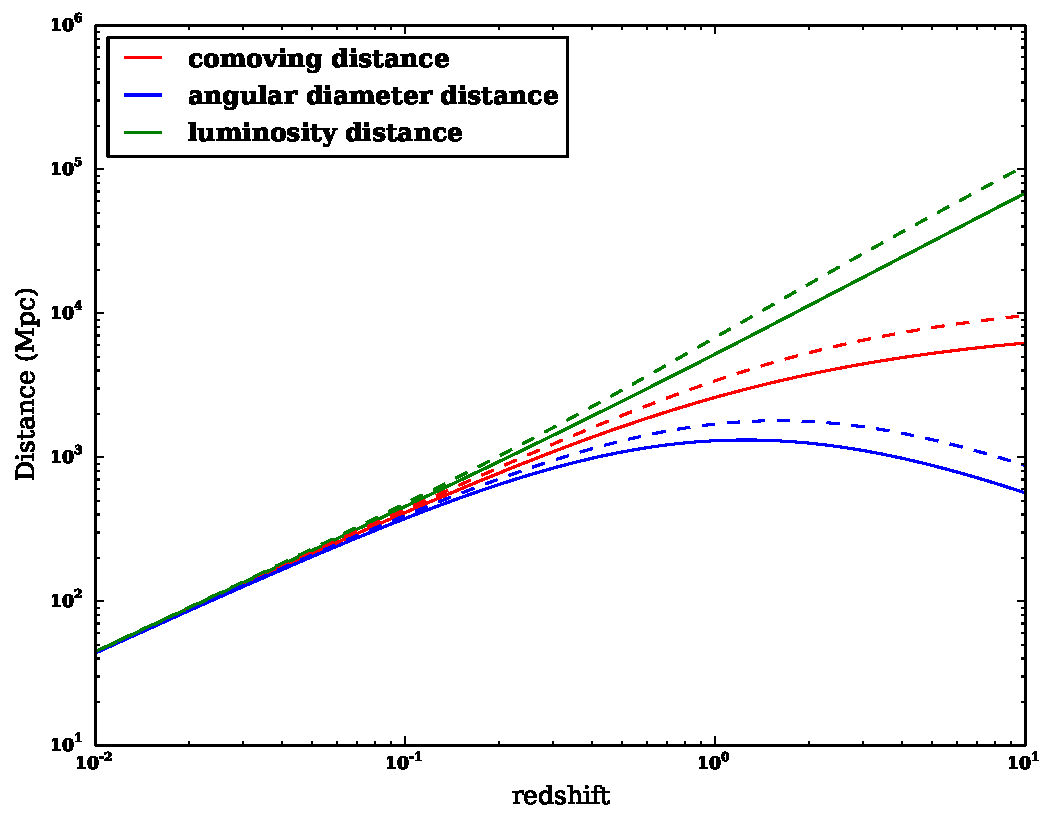
\includegraphics[width = \columnwidth]{figs/dist_redshift.pdf}
 \caption{Cosmological distances as a function of redshift - solid lines represent matter dominated universe and dashed lines represent \citet{planck18-6} cosmology. Measuring distance as a function of redshift provides valuable information on the constituent of the Universe. }
\label{fig:dist}
 \end{figure} 
 Fig. ~\ref{fig:dist} shows cosmological distances as a function of redshift; dashed lines represent the $Planck$ \citep{planck18-6} cosmology and solid lines represent matter only universe. 
 %Its worth here to note that the cosmological distances depend on the underlying cosmology. 
 %In fact the luminosity distances of supernovae were the first observational evidence of dark energy \pending{cite supernovae paper}.
  
 \section{Friedmann Equations}
The mathematical formalism of the universe so far based on the assumption of isotropy and homogeneity in an expanding universe which led us to the FLRW metric.
General theory of relativity relates the dynamics of the background universe to the matter and energy content in the universe via the Einstein Field Equations
\begin{equation}
 R_{\mu \nu} - \frac{1}{2} g_{\mu \nu} R = 8 \pi GT_{\mu \nu}.
\end{equation}
The L.H.S corresponds to the geometry of the universe, while the R.H.S represents the matter and energy content in the universe.
In the above equation $R_{\mu \nu}$ is the Ricci tensor which depends on the metric and its derivatives, R is the Ricci scalar and $g_{\mu \nu}$ is the metric.  The stress energy tensor, $T_{\mu \nu}$, is given by:
\begin{equation}
T^{\mu}_{\nu} = (\rho + P) u^{\mu} u _{\nu } - P \delta^{\mu}_{\nu}
\end{equation}
where $\rho(t)$ and P(t) are the energy density and pressure in the rest frame of the fluid and $u^{\mu}$ is the relative four velocity of the fluid.
Solving the time-time component of the Einstein field equation yields an equation for the evolution of the scale factor,
\begin{equation}
 H^2 = \left ({\dot a \over a} \right )^2 = \frac{8 \pi G}{3} \rho - \frac{k}{a^{2	}}
\label{Fred2}
\end{equation}
while all three spatial components reduce to 
\begin{equation}
\frac{\ddot{a}}{a} = -\frac{4 \pi G} {3} (\rho + 3P )
\label{Fred1}
\end{equation}
where $\rho$ = $\Sigma_{i} \rho_{i}$ and $P$ = $\Sigma_{i} P_{i}$ are the sum of energy density and pressure of all the components in the universe respectively.
 Equations ~\ref{Fred1} and ~\ref{Fred2} are the Friedmann equations governing the evolution of the background universe. \\\\  The average mass density of the Universe required to just halt the expansion of the Universe, it is given by, %For flat universe $k$  =0, it is given by
%  d In a flat universe ($k$ = 0) the kinetic energy of the universe is just enough to over the gravitational pull of the matter; the energy density which satifies this condition is called the critical density
 \begin{equation}
 \rho_{crit}  = \frac{3 H^{2}}{8\pi G}
 \end{equation}
Note that the value of critical density depends on Hubble's constant which is time dependent. The present value of critical density is approximately $10^{-26} kg/ m^{3}$. While this is equivalent to 6 hydrogen atoms per cubic meter, the best achievable terrestrial vacuum is $10^{9}$ atoms per cubic meter. The critical density can be used to define dimensionless density parameters as $\Omega_{i} = \rho_{i}/\rho_{crit}$. Assuming all the components in the universe are perfect isotropic fluids, we can write down the stress energy tensor as
\begin{equation}
T^{\mu}_{\nu} = 
\begin{pmatrix}
-\rho & 0 & 0 & 0 \\
0 & P & 0 & 0 \\
0 & 0 & P & 0 \\
0 & 0 & 0 & P 
\end{pmatrix}
\end{equation}
Using the energy-momentum conservation condition 
\begin{equation}
\dot \rho + 3\,H  (\rho + P) = 0
%\dot{\rho}  + H(3\rho + P)  = 0
\end{equation}
Note that the continuity equation will also hold for individual species as long as we neglect the energy exchange among different components. 
As mentioned earlier the cosmological fluids are expected to obey the equation of state: P = $w$ $\rho$. 
Plugging this in the above equation we can solve for density as function of scale factor
\begin{equation}
\rho(a) \propto \exp \left(-3 \int_1^a {da' \over a'} [1+w(a')] \right)
\end{equation}
For a time-independent equation of state parameter $w$ the above equation reduces to $\rho \propto a^{-3 (1+w)}$. 

The components of the Universe that we know about are:
\begin{itemize}
\item{\textbf{Non relativistic matter}}: For non-relativistic matter such as cold dark matter and baryons the energy density is equal to the rest mass energy. The pressure is much smaller than the energy-density ($P$ << $\rho$). In such cases $w =0$ and the density will scale as $\rho \propto a^{-3}$
\item{\textbf{Radiation and relativistic matter}}:  Pressure is related to the energy-density of relativistic matter as $P = 1/3 \rho$. This includes photons and neutrinos whose density scales with scale factor as $\rho \propto a^{-4}$
\item{\textbf{Dark Energy}}: It is a hypothetical form of energy which is responsible for late time cosmic acceleration. The equation of state parameter depends on the model of Dark Energy and in many of models the equation of state is time dependent. However the current data suggests the value equation of state parameter to be consistent with $w = -1$, with the \citet{planck18-6} indicating $w = -1.04 \pm 0.1$ . Substituting it in the above equation we get $\rho \propto a^{0}$ and hence the cosmic dilution doesn't affect the dark energy density. 
 \end{itemize}
 It is important here to note that the cosmic dilution has different effect on different components. While radiation component is subdominant in today's universe, it played a major role in the early universe. Fig. ~\ref{fig:scaling} shows the energy density of different components as a function of scale factor; as one expects at late times cosmological constant and matter are the dominant components, whereas at earlier times radiation plays a significant role in the evolution of background universe.
 \begin{figure}[ht]
 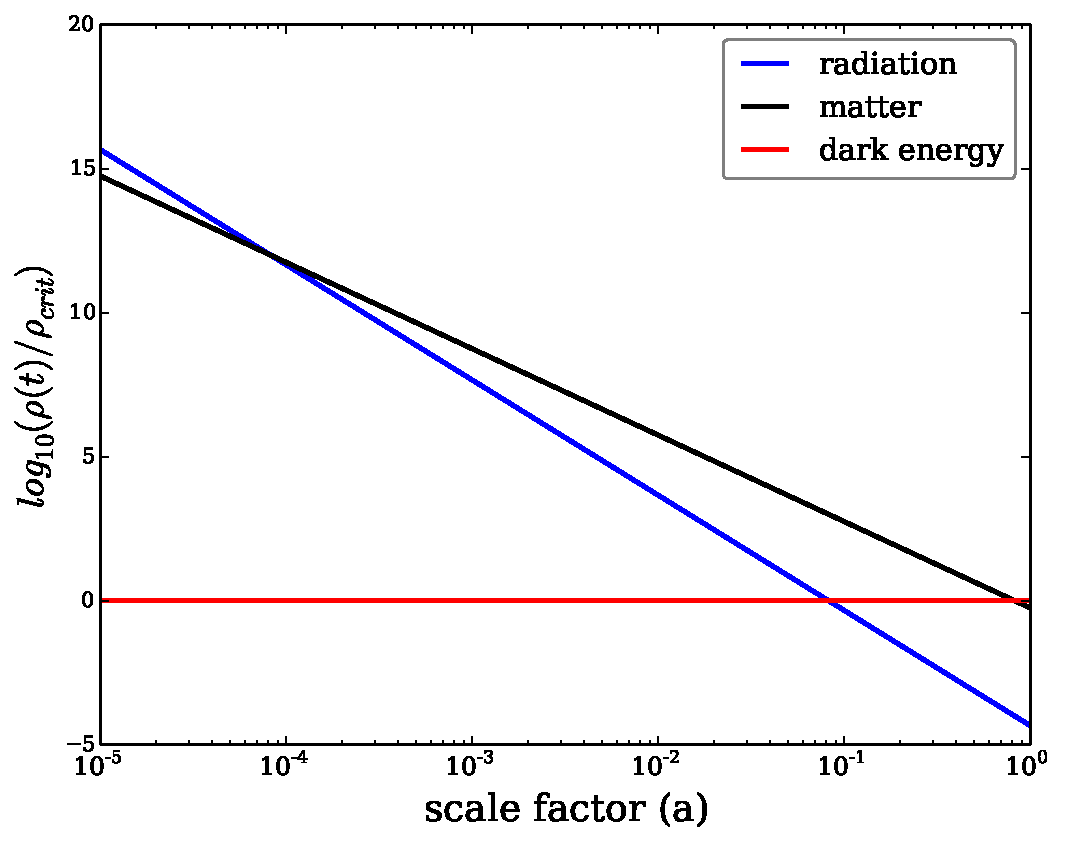
\includegraphics[width = \columnwidth]{figs/dummy.pdf}
 
 \caption{Scaling of various components as function of scale factor (a). While radiation is dominant component in the early universe, dark energy is dominant at present.}
 \label{fig:scaling}
 \end{figure}
With the density scaling relations in hand and substituting a = 1/(1+z), we can rewrite Eqn. ~\ref{Fred2} for a flat universe as 
\begin{equation}
H^{2}(z) = H^{2}_{0} (\Omega_{ro}(1+z)^{4} + \Omega_{mo}(1+z)^{3} + \Omega_{\Lambda}) 
\end{equation} 
where $\Omega_{ro}$,$\Omega_{mo}$ and $\Omega_{\Lambda}$ are the density parameters of radiation, matter and dark energy respectively. 
\iffalse{
 \section{Cosmic Inventory}
The above theoretical framework provides the evolution of different components as a function of scale factor. Now we look at the observational constraints obtained on these parameters. CMB temperature is measured precisely by the FIRAS instrument \cite{mather94} on COBE satellite \cite{fixsen96b}, $T = 2.725$ K $\pm$ 0.002K. %While neutrinos also contribute to radiation density, cosmic neutrinos have not been observed yet. 
For bosons such as photons the energy density as a function of temperature is given by 
\begin{equation}
\rho_{\gamma} = \frac{\pi^{2}}{15} T^{4}
\end{equation} 
which corresponds to 
\begin{equation}
\Omega_{\gamma} = \frac{\rho_{\gamma}}{\rho_{crit}} = 5.04 *10^{-5}
\end{equation}

Unlike photons the energy density of baryons cannot be obtained by measuring its temperature, it needs to be measured directly. 
There are two main independent ways to measure the baryon density: 
\begin{itemize}
\item Cosmic Microwave Background (CMB): by measuring the amplitude of the first and second peaks of CMB power spectrum
\item  Big Bang Nucleosynthesis (BBN): by measuring the primordial deuterium abundance.
\end{itemize}
From CMB power spectrum analysis we have $\Omega_{b} h^{2}$ = $0.0224 \pm 0.0001$  \cite{planck16-8} and that from BBN is $0.0226 \pm 0.00034$ \cite{cooke16}. Both of these measurements agree with each other remarkably well within error limits.


Dark matter forms 85\% of total matter content in the universe. Unlike baryons, dark matter doesn't interact with the radiation. 
As dark matter interacts only gravitationally, by measuring the gravitational field in a given system we can infer the total mass content. 
One of the ways to measure the total matter (dark matter + baryon) is by using galaxy cluster gas mass fraction. 
Galaxy clusters (detailed review is in next chapter) are so large that the ratio of gas mass to that of total cluster mass is expected to reflect the ratio baryon to the total mass in the universe\cite{white93a,grego01}. Constraints on dark matter density as measured by $Planck$ is $\Omega_{dm} h^{2} =  0.120 \pm 0.001$ \cite{planck16-8}.

As per current cosmological observations the major contribution for the energy density content in the universe is from dark energy. There are several observational probes to constrain this mysterious component which is responsible for the late time acceleration of the universe.  The first direct observational evidence is from type Ia supernovae. Supernovae have constant intrinsic luminosity and are known as standard candles. 
Cosmologists measured the luminosity distance (~\ref{eq:luminosity_dist}) of type Ia supernovaes as function of redshift to constrain $\Omega_{\Lambda}$  $\approx$ 0.7\citep{knop03}.
}\fi

\section{Cosmic Microwave Background}
Cosmic Microwave Background (CMB) was theoretically predicted by George Gamov in 1940s as an observational relic of Hot Big Bang model \citep{article46}. 
It was observed accidentally by Arno Penzias and Robert Wilson in 1964 at the Bell Laboratories for which there were awarded Nobel prize in physics in 1978 \citep{penzias65}. Almost three decades after its discovery, Cosmic Background Explorer (COBE) detected anisotropies in CMB at a tiny level of 10 in a million. Far-Infrared Absolute Spectrophotometer (FIRAS), an instrument mounted on COBE measured the black body spectrum of CMB \citep{mather94}. %temperature of CMB to be  $\sim$ 2.7K. 
Since then a number of experiments have been designed to measure the anisotropies in the CMB.

High density and temperature of the early universe ensured that all the components interacted with each other multiple times remaining in thermal equilibrium. 
Photons ($\gamma$), protons (p) and electrons (e) were tightly coupled into a state called photon-baryon plasma; proton and electrons interacted with each other through Coulomb scattering and photon interacted with electrons through Thompson scattering:
\begin{eqnarray}
\cee{p + e^{-} <=> H + \gamma}
\label{Coulomb}\\
\cee{\gamma + e^{-} <=> e^{-} + \gamma}
\end{eqnarray} 
As the universe expands the mean energy density dilutes and the temperature decreases. When the temperature falls below the ionization energy of hydrogen, E < 13.6 eV the reaction in Eq.~\ref{Coulomb} thermodynamically favours to  $\cee{p + e^{-} -> H + \gamma}$ \footnote{To be precise, recombination occurs at slightly lower temperature (~1MeV) due to the large over abundance of photons with respect to baryons}. This results in the creation of neutral hydrogen atoms and the electron density decreases, which results in the decoupling of photons from the baryons. This epoch is called the epoch of recombination; observations determine that it happened at redshift of  $z$ = $1089.90 \pm 0.23$ \citep{planck18-6}. 

As a first light from the early universe, the CMB provides a wealth of cosmological information. The theory of inflation is able to describe the homogeneity measured in the CMB. The inhomogeneties are only of order of 10 in a million which can be directly measured from the observed anisotropies in CMB. %Over the evolution of the universe slightly over dense regions of the early universe collapsed gravitationally to form the large scale structures that we see today. Analysing these structures involve complicated non-linear physics, however, CMB can be analysed linearly. In addition to that, $z \sim 1100$ provides long lever arm on the geometry of the universe.

\begin{figure}[ht]
\includegraphics[width = \columnwidth]{figs/CMB_map.pdf}
 \label{cmb map}
 \caption{CMB anisotropies as observed by $Planck$ satellite. Credits: ESA/$Planck$ collaboration}
\end{figure}
\iffalse{
\section{Boltzmann equations}
\label{eqns}
In the early universe photons, baryons, and dark matter are tightly coupled to each other in a complicated way. 
The systematic way to understand these couplings is by using Boltzmann equations. 
Boltzmann equations are easier to solve in Fourier space, as different Fourier modes evolve independently in linear approximation. 
This section closely follows \pending{Scott and Dodelson}, here I summarize the Boltzmann equations for cold dark matter, photons, and baryons which were the dominant component of the universe at recombination.


The evolution of photon distribution is coupled to electrons and metric. Photon Boltzmann equation in the Fourier space is given by:
\begin{equation}
\dot{\tilde{T}} + i k(\hat{k}. \hat{p}) \tilde{T} + \dot{\tilde{\Phi}} + i k (\hat{k}.\hat{p}) \tilde{\Psi} = \dot{\tau}[\tilde{T_{0}} - \tilde{T} + (\hat{k}.\hat{p})\tilde{v_{b}}]
\end{equation}
where T represents the photon temperature, $\hat{p}$ is the photon direction, $v_{b}$ is the electron velocity, and $\tau$ is the optical depth.
Variables with $\tilde{}$ denotes Fourier transform, ones with $\dot{}$ denotes derivative with respect to conformal time $\eta$.
$\dot{\tilde{\phi}}$ and $\dot{\tilde{\psi}}$ represent the conformal time derivative of the metric. 

Cold dark matter (CDM) evolution is the simplest among all as it has only two free parameters velocity and density. 
CDM Boltzmann equation is given by:
\begin{eqnarray}
\dot{\tilde{\delta}} + ik\tilde{v} + 3 \dot{\tilde{\Phi}} = 0\\
\dot{\tilde{v}} + \frac{\dot{a}}{a} \tilde{v} + ik \tilde{\Psi} = 0
\end{eqnarray}
where $v$ is the dark matter velocity, a is the scale factor, and $\delta$ is the fractional dark matter over density 
\begin{equation}
\delta = \frac{\delta \rho}{\rho} 
\end{equation}
$\rho$ is the dark matter density.

Proton and electrons are tightly coupled to each other by Coulomb forces. In addition to that the electrons also interact with photons through Thompson scattering. 
Both protons and electrons are analysed together as baryons, the Boltzmann equation for baryons is given by
\begin{eqnarray}
\dot{\tilde{\delta_{b}}} + ik\tilde{v_{b}} + 3 \dot{\tilde{\Phi}} = 0 \\
\dot{\tilde{v_{b}}} + \frac{\dot{a}}{a} \tilde{v_{b}} + i k \tilde{\Psi} = \dot{\tau}\frac{4\rho_{\gamma}}{3\rho_{b}} [3i\tilde{T_{1}} + \tilde{v_{b}}]
\end{eqnarray}
where $\rho_{\gamma}$ and $\rho_{b}$ are the photon and baryon density respectively; $T_{1}$ is the first moment of photon temperature. 

All the above Boltzmann equations can be solved numerically to a great precision for a given cosmological model by using publically available codes such as CAMB \citep{lewis00} and CMBFAST \citep{seljak96}.
\begin{figure}[ht]
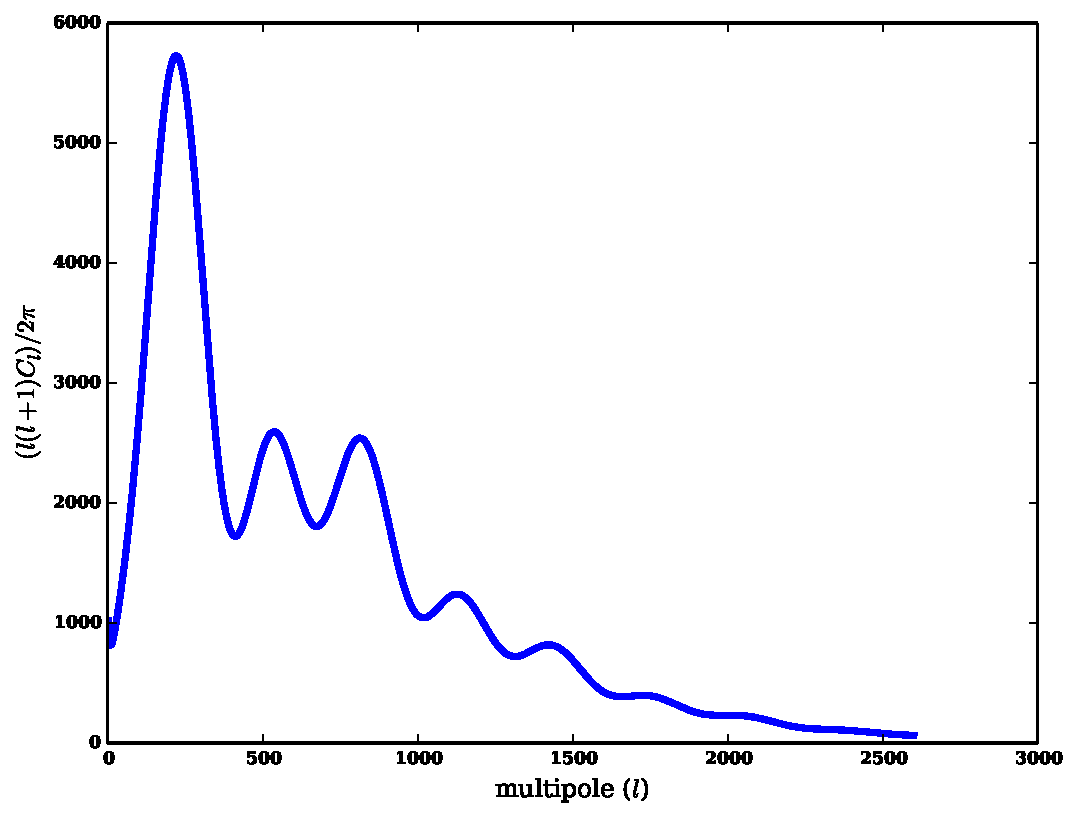
\includegraphics[width = \columnwidth]{figs/cmb_ps.pdf}
\caption{Angular power spectrum of CMB primary temperature anisotropies for $Planck$ cosmology \citep{planck18-6}.}
\label{fig:cmb_ps}
\end{figure}
}\fi
\section{Temperature primary anisotropies}
 The measured CMB temperature in a given direction $\hat{n}$ can be written as:
\begin{equation}
T = T_{0}\left(1+ \vec{\beta}.\hat{n} + \frac{T(\hat{n})}{T_{0}}\right)
\end{equation}
where $T_{0}$ is the average CMB temperature, $\vec{\beta} $ is the dipole term due to the relative velocity of Earth with respect to Hubble flow. Here $\beta$ is equal to $\frac{\vec{v}}{c}$ where $\vec{v}$ is the Earth's relative velocity. 
The last term in the equation represents the anisotropies in the CMB which here after we denote by $\Phi(\hat{n})  = \frac{T(\hat{n})}{T_{0}}$. 
Note that in the above equation we have ignored foregrounds, systematics, and experimental noise. %The oder of the anisotropies ($\phi$) is two orders of magnitude smaller than effect due to doppler boost. 

Given the stochastic nature of fluctuations in CMB, we cannot predict the value of temperature at a given location. However, we can predict the statistical properties. 
As an function on the surface of sphere, CMB fluctuations can be decomposed in terms of spherical harmonics as follows:
\begin{eqnarray}
\Phi(\hat{n}) = \Sigma_{l} \Sigma_{m} a^{T}_{lm} Y_{lm} (\hat{n}) \\
a^{T}_{lm} = \int d\Omega \Phi(\hat{n}) Y_{lm} (\hat{n})
\end{eqnarray}
where $Y_{lm}$ are the spherical harmonic basis, %used to define function on a sphere
$a^{T}_{lm}$ are the harmonic coefficients. 
It is important to note here that angular scale $\theta$ is related to multipole $l$ as $\theta \sim 1/l$. 

The randomness of the fluctuations wont let us predict the value of the harmonic coefficient $a^{T}_{lm}$. However, theories do predict the distribution from which the $a^{T}_{lm}$ are picked. In the inflationary paradigm CMB fluctuations are realisations of a  Gaussian random field, meaning that the harmonic coefficients are drawn from random Gaussian distribution\footnote{It must be noted that most of the inflationary models predict a small amount of non-Gaussianity.}. The harmonic coefficients satisfy 
\begin{eqnarray}
\langle a^{T}_{lm} \rangle = 0,\\
\langle a^{T}_{lm} a^{T*}_{l'am'}\rangle = \delta_{l l'}\delta_{m m'} C^{TT}_{l},\\
a^{T}_{l-m} = (-1)^{m}a^{T*}_{lm}
\end{eqnarray}
where $\langle \rangle$ denotes the ensemble average over many realisations, $C^{TT}_{l}$ is the angular power spectrum of CMB. 

Our universe is only one of many realisations of the Gaussian random field, so we face fundamental limits on the knowledge available. This is known as cosmic variance.
 However, we can still calculate the angular power spectrum.
The idea is to replace the ensemble average with the spatial sample average i.e averaging over $2l +1$ samples. 
\begin{equation}
\hat{C}^{X}_{l} = \frac{1}{2l +1}\Sigma_{m} |a^{X}_{lm}|^{2}
\end{equation}
where X $\epsilon$ (T,E,B) - T is the temperature mode and E, B are the polarisation modes .
This measured power spectrum is fitted to the theoretical power spectrum to extract cosmological information. For historical reasons the CMB power spectrum is conventially parameterized as 
 \begin{equation}
 D_{l} = \frac{l(l+1)}{2\pi} C_{l}.
 \end{equation}
 
 The theoretical CMB power spectrum for standard $\Lambda CDM$ cosmology as obtained from CMBFAST \citep{seljak96} is show in Fig. ~\ref{cmb_ps}. A wealth of cosmological information can be obtained from CMB power spectrum and below I discuss three main features (it closely follows \citet{douglas2010}):
 
\begin{figure}[ht]
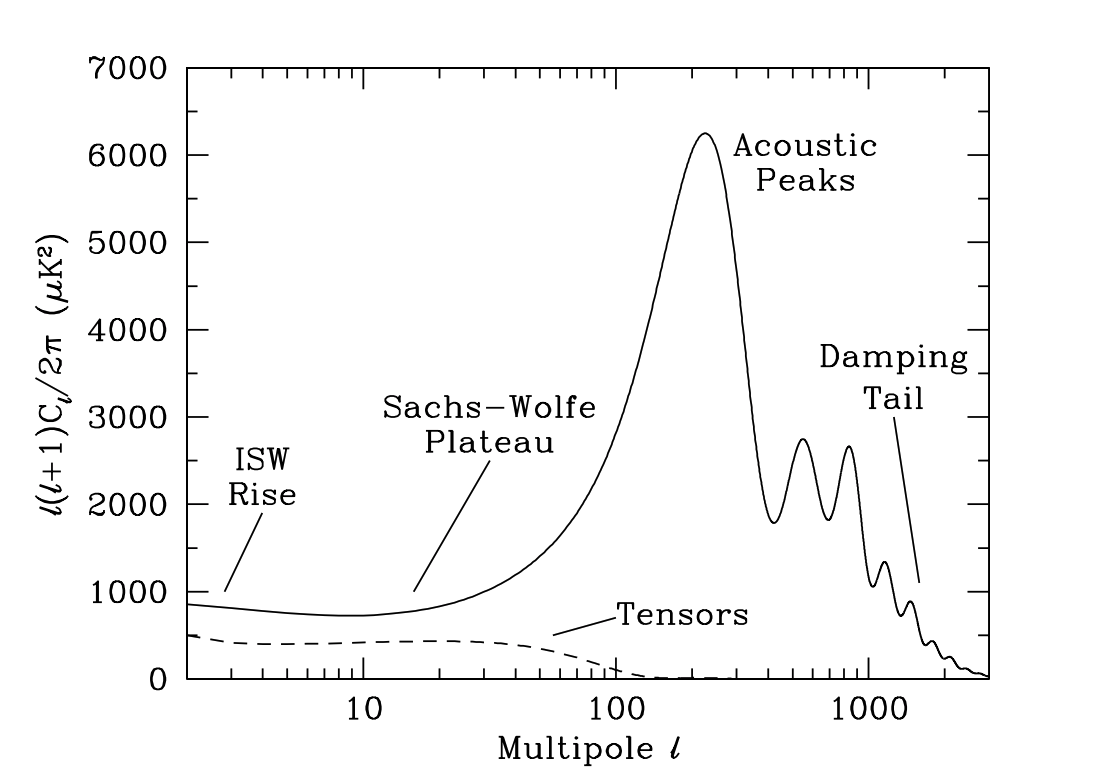
\includegraphics[width = \columnwidth]{figs/cmb_ps_sd.png}
\caption{The theoretical CMB power spectrum as obtained from CMBFAST \citep{seljak96}}
\label{cmb_ps}
\end{figure}

 \textbf{Sachs-Wolfe Plateau:}
 
 The horizon scale at last scattering surface corresponds to multipole $l \approx 100$. At these scales the anisotropies have not evolved significantly and hence faithfully trace initial condition. $\delta T/ T \approx  1/3 \delta \phi c^{2}$, where $\delta \phi $ is the perturbation to the gravitational potential evaluated on the last scattering surface (LSS) \citep{sachs67}.
 
 \textbf{Acoustic oscillations:}
 
On sub-degree scales, corresponding to multipole range $ 100 \le l \le 1000 $, the rich structure in the power spectrum is due to gravity-driven acoustic oscillations occurring before the atoms in the Universe became neutral. Perturbations inside the horizon at last scattering have been able to evolve causally and produce anisotropy at the last scattering epoch, which reflects this evolution. The frozen-in phases of these sound waves imprint a dependence on the cosmological parameters, which gives CMB anisotropies their great constraining power. Location and height of acoustic peaks are sensitive to various cosmological parameters especially curvature of the Universe, dark energy, amount of baryons, optical depth, and dark matter \citep{hinshaw13,planck18-6}. 
 
\textbf{Damping tail:}

The recombination process is not instantaneous, giving a thickness
to the last scattering surface. This leads to a damping of the anisotropies at the highest $l$s, corresponding to scales smaller than that subtended by this thickness. One can also think of the photon-baryon fluid as having imperfect coupling, so that there is diffusion between the two components, and hence the amplitudes of the oscillations decrease with time. These effects lead to a damping of the $C_{l}$s, sometimes called Silk damping \citep{silk68}, which cuts off the anisotropies at multipoles above about 2000 \citep{keisler11,story13,das11b,reichardt09a}.   

The CMB interacts with the intervening medium (between last scattering surface and us) and this imprints secondary anisotropies. Secondary anisotropies also provide wealth of cosmological information especially on structure formation and epoch of reionisation \citep{lueker10,shirokoff11,flower10,das11}. 

\section{CMB polarisation}
\begin{figure}[ht]
 \includegraphics[width = \columnwidth]{figs/quadrupole.pdf}
\caption{The above figure depicts important scenarios as experienced by an electron at the time recombination; it is adopted from the works of \cite{hu97d} and \cite{dodelson_book}. }
\label{quadrupole}
\end{figure}

The CMB is partially polarised linearly at the 10\% level due to the Thompson scattering of photons by electrons at the surface of last scattering. 
Only quadrupole anisotropy is responsible for CMB polarisation as shown in Fig. ~\ref{quadrupole}. 
 The Fig. ~\ref{quadrupole} represents important scenarios experienced by electron at the time of recombination. Red and blue represent relatively hot and cold photons respectively; green represents the average temperature. 
 Image on the top left represents the isotropic scenario which results in no net anisotropy.
 On the top right is that of dipole anisotropy which also results in no net polarisation. 
 Only the quadrupole anisotropy which is shown in the bottom panel results in net linear polarisation. 


The polarisation pattern on the CMB sky can be decomposed into curl-free E-modes, and
divergence-free B-modes. This is similar to Maxwell?s equation where the curl of the electrostatic
field, and the divergence of the magnetic field are zero. The reason the polarisation
patterns are called E, B modes is because of this similarity to electromagnetism.
\begin{eqnarray}
\vec{\nabla} \times \vec{E} = 0\\
\vec{\nabla} . \vec{B} = 0
\end{eqnarray}

The most important reason for this decomposition is that the scalar perturbations only
generate E-modes but does not generate B-modes, and the tensor perturbations generate both
E, and B-modes in equal amounts.
 %Before recombination photons and electrons were tightly coupled resulting no net local anisotropy. 
%However, during the period of recombination there is slight anisotropy between photons and free electrons. 
Though CMB polarisation signal is weak compared to its temperature counterpart, it provides invaluable information on inflation and on late time evolution of universe through its lensing effects and the imprint of primordial gravitational waves on tensor B-modes
In addition to that, foregrounds are only partially polarised.
The CMB polarisation was first detected observationally by Degree Angular Scale Interferometer (DASI) in 2002 \citep{kovac02}.
Since then measurement of CMB polarisation has been done by SPT \citep{henning18,sayre19,keisler15}, ACT \citep{louis16,naess14}, $Planck$ \citep{planck19},  BICEP2/Keck \citep{bicep18,bicep15}, and POLARBEAR \citep{polarbear2014b,wald2019}. %numerous experiments which have measured CMB polarisation \citep{sayre19,henning18,bicep18,keisler15,polarbear2014b}.

 
 
 \section{Other cosmological probes}
 
 In addition to CMB there are other cosmological probes which provide invaluable and complementary insight into the standard model of cosmology. Below I provide a very brief discussion of other cosmological probes.
 
 
 \textbf{Supernovae:}
 
Type Ia supernovaes are excellent standard candles for measuring the expansion history of the Universe and provided the first direct evidence of dark energy \citep{riess98,perlmutter99a,perlmutter99b}. Theoretical models suggest that these ``standard candles'' arise because of thermonuclear explosion of a carbon-oxygen white dwarf that has grown to the Chandrashekar mass.
%Type Ia supernovae are thought to be result of explosion of white dwarf in a binary system. 
These events have well defined Hubble diagram whose intercept provides a robust measurement of  Hubble constant. The value of hubble constant measured using Type Ia supernovae data from Dark Energy Survey is $H_{O} = 67.8 \pm 1.3 \; \si{\km\per\s}\si{\per\mega\parsec}$ \citep{macaulay2018}. %will and by measuring their brightness we can measure how far supernovae are  and hence the expansion of the Universe. 
 


 \textbf{Baryon Acoustic Oscillations:}
  
While supernovae acts as ``standard candles'', Baryon Acoustic Oscillations (BAO) acts as standard rulers in cosmology. 
 They are the frozen relics left over from the pre-decoupling universe. As such, probing the BAO scales at different times provides valuable cosmological information. 
 The best measurement BAO scale comes from CMB anisotropy measurements at redshift $z \approx 1100$ \citep{planck18-6}. BAO are also present in
the distribution of matter, and there are measurements at low redshifts using the clustering of galaxies \citep{beutler11,ross15,alam16}.
BAO data can only constrain a combination of the size of the sound horizon and the expansion rate of the Universe ($H_{o}$). Usually CMB anisotropy measurements are used to break this degeneracy. Using the Big Bang Nucleosynthesis prior and latest data from eBOSS DR14, \citet{andrei14} measured $H_{O} = 67.6 \pm 1.1 \si{\km\per\s}\si{\per\mega\parsec}$. 
 
 
 %\textbf{Redshift Space Distortions (RSD}
  
 


%  -------  Relevant theory  -------  
\setcounter{chapter}{1} %2
		 \chapter{Maximum Likelihood Estimator}
\label{ch:MLE}
\section{Overview}
The path of the Cosmic Microwave Background (CMB) photons gets bent due to the intervening galaxy cluster. 
Distortion in the background CMB is of the order of few arcminutes for a massive galaxy cluster.
On the galaxy cluster length scales (order of arcminutes) CMB can be approximated as a gradient due to diffusion damping \citep{silk96}. 
Gravitational lensing induces a dipole kind of structure on top of the gradient with hot and clod spots swapped. 
The strength of the gravitational lensing signal (lensing dipole) is directly proportional to the background gradient and the cluster mass. 
As polarisation signal is an order of magnitude smaller than temperature, lensing signal in polarisation is also an order of magnitude smaller than that of temperautre. 
Fig ~\ref{fig:lensing_signal} shows the lensing signal for a cluster of mass $5*10^{14}$ $M_{\odot}$ and at redshift of $z$ = 0.7.
On the left panels we have the background CMB gradient for the temperature and polarisation stokes Q and U parameters, on the middle panel we have the corresponding lensed maps; on the right panel we have the lensing dipole signatures.

Lensing remaps the unlensed CMB temperature and polarisation fields based on the gravitational deflection angle of the cluster. 
\begin{eqnarray}
T(\hat{n}) = \tilde{T}(\hat{n} + \alpha(\hat{n}))\\
Q(\hat{n}) = \tilde{Q}(\hat{n} + \alpha(\hat{n}))\\
U(\hat{n}) =  \tilde{U}(\hat{n} + \alpha(\hat{n}))
\end{eqnarray}
where T represents the temperature field, Q and U are the stokes polarisation parameters respectively. 
Tilde represents the unlensed fields, $\alpha(\hat{n})$ is the deflection angle vector due to the cluster lensing along the $\hat{n}$ direction. 
Deflection angle is related to gravitational potential as $\nabla \phi (\hat{n})$ and is directly proportional to the mass of the cluster.

In literature, there are several methods to extract lensing singal from CMB data. 
During my thesis, I mainly worked on two methods for extracting lensing signal from the observed CMB data: Maximum Likelihood Estimator (MLE) and Quadratic Estimator (QE). 
In this chapter, I will explain the MLE in detail. While we compare the results of MLE with QE, QE is explained in detail in next chapter.
\begin{figure}[t]
\begin{center}
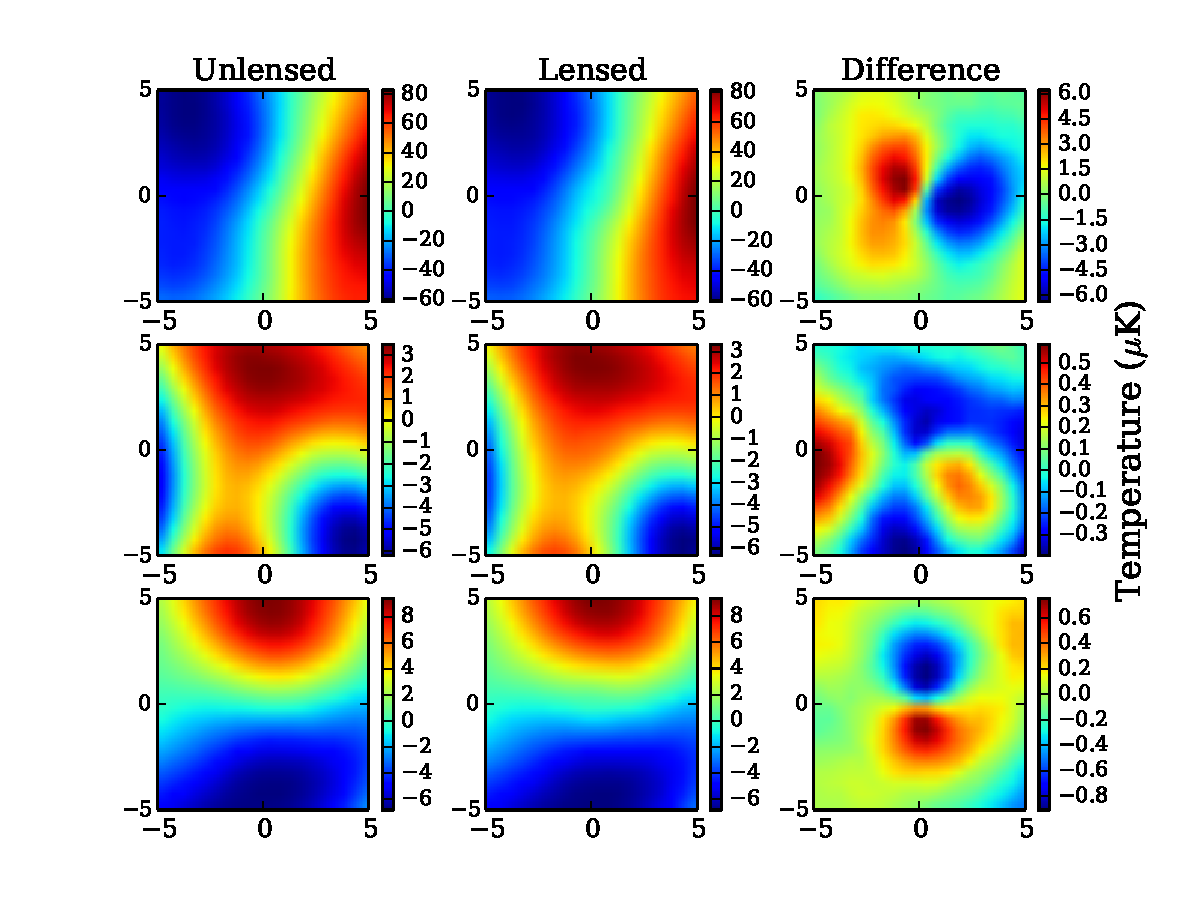
\includegraphics[width=\linewidth, keepaspectratio]{figs/lensing_signal.pdf}
 \caption{Lensing effect on CMB due to a galaxy cluster of mass $5\times 10^{14}$ \msolar.
  On the top panel we show the effect of cluster lensing on CMB temperature field.
  Bottom two panels are for the stokes Q and U parameters. 
 } 
\label{fig:lensing_signal}
\end{center}
\end{figure}

\section{Maximum Likelihood Estimator}
\label{sec_MLE}
Gravitational lensing by a galaxy cluster induces extra pixel-pixel correlations. 
MLE extracts the lensing signal by modeling these pixel-pixel correlations in the form of covariance matrix.


\subsection{Covariance matrix calculation}
Here, I explain the calculation of covariance matrix which will act as the model.
The distortion of CMB due to a galaxy cluster is of the order of arcminutes; much of the lensing is within 10\am from cluster center.
For covariance matrix calculation we take central \smallboxsize cutout.
We also checked that by increasing the boxsize to 14\am we gain an improvement in a SNR of less than 1\%, however, that the increases the computational complexities. 


 We calculate the covariance matrix by using a set of simulated skies. 
 To calculate the simulated lensed CMB sky, first we generate the large-scale structure lensed CMB power spectra ($C^{TT}_{l}, C^{TE}_{l}, C^{EE}_{l},$ and $C^{BB}_{l}$) form CAMB for the $planck$ 2015 cosmology \citep{planck15_13}.  
 We generate Gaussian random realisations with these power spectra on a 50\am X 50\am box. 
 Q and U maps are generated by using E and B maps as
 \begin{eqnarray}
Q = E + B\\
U = E + B
 \label{eq:coord_trans}
 \end{eqnarray}
 
 \pending{correct the equations}
 While we only use  \smallboxsize  for final calculations we simulate a bigger box (50\am) to take into account the large scale gradient.
 These Gaussian realizations are then lensed by an assumed galaxy cluster density profile (explained in next section). 
 
 With simulated lensed CMB maps in hand we calculate the covariance matrix as follows
 \begin{eqnarray}
\Sigma_{lens}(M,z) & = & \left<(\textrm{\textbf{G}} - \left<\textrm{\textbf{G}}\right>) (\textrm{\textbf{G}} - \left<\textrm{\textbf{G}}\right>)^{T}\right>\\
  =   \frac{1}{n-1}\sum\limits_{i = 0}^{n} (\textrm{\textbf{G}}_{i} - \left<\textrm{\textbf{G}}\right>) (\textrm{\textbf{G}}_{i} - \left<\textrm{\textbf{G}}\right>)^{T} %(\textrm{\textbf{G}}_{i} - \left<\textrm{\textbf{G}}\right\
%s>)^{T},
\label{eq_lensed_cmb_cov_mass_z}
\end{eqnarray}
 where vector $G_{i}$ is either the polarisation or temperature simulated data for $i^{th}$ sky realisation. 
 The number simulated skies depend on the number of degrees of freedom in the covariance matrix. 
 In our case, we concatenate Q and U maps for our polarisation estimator for which the covariance matrix is a 800 X 800 matrix. 
 Number of simulations scale as twice the number of elements in the covariance matrix; we found 1,30,000 simulations are sufficient for recovering cluster masses without any bias. 
  We then multiply Hartlap correction term $\frac{(n_{sims} -n_{d} -1)}{n_{sims}}$, where $n_{sims}$ is 1,30,000 and $n_{d}$ is the length of the vector 400(800) for T(QU), to remove any possible bias in $\Sigma^{-1}_{lens}$ due to the limited number of simulations. 
  
 We also use these simulated skies to quantify the effects of statistical and systematic uncertainties.
 There are several astrophysical sources which act as a systematic bias and foregrounds for the CMB-cluster lensing analysis. 
 In this work we consider clusters own SZ effects such as thermal Sunayev-Zel'dovich (tSZ) and kinematic Sunayev-Zel'dovich effects. 
 %tSZ is in explained in detail in the next chapter. 
 Along with these SZ effects we have also considered sources which are uncorrelated with cluster such as tSZ effect from other halos, dusty star forming galaxies (DSFGs), and radio galaxies.
 In appendix, we provide in more details about the addition of these foregrounds to simulated skies.
 
 In this chapter we have considered only simulated data to check the efficiency of MLE. 
 Unless otherwise mentioned all the clusters are simulated at a mass of $M_{200} = 2*10^{14}$\msolar \pending{footnote} and at redshift of 0.7.
 For covariance matrix calculation we simulate the skies at redshift of $0.7$ with mass resolution of $2*10^{12}$\msolar. 
 Note that such fine gridding might not be computationally feasible for data where the clusters span wide range of masses and redshifts.
 An optimal solution would be generate the covariance matrices on coarser grid of mass and redshift and then interpolating it on a finer grid.
 
 
 
  
   
  
  \subsection{Likelihood Estimation}
  With the covariance matrix in hand we calculate the likelihood given the data as follows 
  
  \begin{equation}
  -2lnL(d|\Sigma_{lens}) = ln |\Sigma_{lens}| + d^{T} \Sigma^{-1}_{lens} d
  \end{equation}
  where the data vector $d$ is the pixel values of the observed T or Q/U maps.
  The pixel values are defined as the variations from the mean CMB temperature (polarisation) and hence have zero mean.
  
  %Since the majority of the lensing singal is within few arcminutes from the cluster center, we carry out the lensing analysis within \smallboxsize of the cluster center to simplify and speed up the analysis. 
  %We also checked that by increasing the boxsize to 14\am we gain an improvement in a SNR of less than 1\%, however, that the increases the computational complexities. 
  As pointed out earlier, the lensing signal of a single galaxy cluster is much weaker to be detected. 
  We stack many clusters to increase SNR (signal to noise ratio) to a reasonable level
  \begin{equation}
  -2ln L(d| \Sigma_{lens})_{tot} = \Sigma^{n}_{i =0} w_{i} [ln |\Sigma_{lens}| + d^{T}_{i} \Sigma^{-1}_{lens}  d]
  \end{equation}
  where n is the total number of clusters in the sample, $w_{i}$ is the weight for the $i^{th}$ cluster which depends on the survey noise etc.. 
  In this chapter as we are using simulated clusters, we assign uniform weights to each cluster.  

  \subsection{Lensing convergence profile}
  In order to lens the simulated CMB sky we need to know the lensing deflection angle.
  Deflection angle depends on the lensing convergence profile as follows:
\begin{equation}
 \alpha = \nabla. k = -\nabla^{2} \phi
 \end{equation}
 where $\alpha$ is the deflection angle, $k$ is the lensing convergence profile, and $\phi$ is the lensing potential.
 For a symmetrical density profiles, the lensing convergence profile is equal to the ratio of surface mass density over the critical density of the Universe at the cluster redshift $k = \frac{\sigma(x)}{\sigma_{crit}}$.
 
The surface mass density or also know as the projected mass density of the halo is obtained by integrating the halo density profile along the line of sight. 
 \begin{equation}
 \sigma(x) = 2 \int^{\inf}_{0} \rho(r) ds
 \label{eq:surface_density}
 \end{equation}
 where r is the radial distance, x is the corresponding 2D planar distance and s is distance along the line of sight with s =0 being the plane of the cluster.
 The critical surface density of the Universe at cluster redshift is given by
 \begin{equation}
 \sigma_{crit} = \frac{c^{2}}{4\pi G} \frac{D_{cmb}}{D_{clus}D_{cmb,clus}}
 \end{equation}
 where $D_{cmb}$ is the comoving distance to the epoch of recombination (z= 1100), $D_{clus}$ is the comoving distance to the cluster (in our case comoving distance to the redshift), and $D_{cmb,clus}$ is the comoving distance between the CMB and the cluster.
 
 Unless otherwise mentioned, I define all the cluster quantities in the chapter with respect to $R_{200}$, which is defined as the radius within which the mean cluster density is 200 times the Universe critical density at cluster redshift $\rho^{z}_{crit}$. $M_{200}$ will be 
 \begin{equation}
 M_{200} = \int^{R_{200}}_{0}  4\pi x^{2} \rho(x) dx
 \end{equation}
 By definition $M_{200}$ is also given by
 \begin{equation}
 M_{200} = \frac{800\pi}{3} R^{3}_{200} \rho^{3}_{crit}
 \end{equation}
 
 The above mathematical equations hold for any spherically symmetric halo, now we move on to a specific case of Navarro Frenk White (NFW) halo density profile.
 In the NFW profile, the density of the dark matter halo as function radius is given by:
 \begin{equation}
 \rho(r)= \frac{\delta_{c}\rho^{z}_{crit}}{(\frac{r}{R_{s}})(1+\frac{r}{R_{s}})^{2}}
 \end{equation}
 where $\delta_{c}$ is the characteristic over-density, $R_{s}$ is the characteristic scale radius, and $c$ is the dimensionless concentration parameter.
 The dimensionless over-density is given by $\delta_{c} = \rho_{0}/\rho^{z}_{crit}$, where $\rho_{0}$ is the cluster central density and  $\rho^{z}_{crit}$  is the crititcal density of the universe at cluster redshift.
 Plugging the above equation in ~\ref{eq:surface_density}, we get the surface density for the NFW halo. 
 By slightly change the variables of integration as $s=\sqrt{r^{2} - x^{2}}$ and $ds = \frac{rdr}{\sqrt{r^{2} - x^{2}}}$ we obtain:
 \begin{equation}
 \Sigma(x) = 2\delta_{c} \rho^{z}_{crit} R^{3}_{s} \int^{\inf}_{x} \frac{1}{r(R_{s} + r)^{2}} \frac{rdr}{\sqrt{r^{2} - x^{2}}}
 \label{eq:sr_den}
 \end{equation}
 The scale radius is related to the concentration parameter as follows:
 \begin{equation}
 c = \frac{R_{200}}{R_{s}}
 \end{equation}
 In this chapter we have set $c = 3.0$ following \cite{bhattacharya13}.
 The ~\ref{eq:sr_den} can be solved analytically and the explicit closed-form expression for the NFW case has been given by \cite{bartelmann96}.
 Unless otherwise mentioned we consider the galaxy clusters to follow NFW profile, however,  the mathematical framework described above can be applied any halo density profile. 
 
 
 \section{Results}

 In this section first we validate our pipeline using simulations, we report the expected mass uncertainties for the polarisation and temperature MLE. 
 Then we compare the performance of MLE and QE for ideal simulations by only vary the experimental noise levels and not including any galactic or extra galactic foregrounds. 
 Later, we compare the performance of the estimators in the presence of foregrounds. 
 In this chapter all the results are for a set of 100,000 simulated clusters (expected number of clusters for CMB-S4) each at a mass of $2\times10^{14} M_{\odot}$ and at redshift of 0.7.
 To obtain the lensing significance, we calculate the ratio of combined likelihood at zero mass to that of maximum likelihood:
 \begin{equation}
 \lambda = \frac{L (M_{200} =0)}{max(L(M_{200}))}
 \end{equation} 
 According the Wilk's theorem, in many cluster limit $\lambda $ follows chi-square statistic with one degree of freedom ($M_{200}$ in our case).
 The detection significance reported in this chapter is equal to $-2 ln (\chi)$
 Similarly, we obtain the errors on mass estimate by calculating masses at which $-2lnL(M_{est}) + 2 ln L (M_{200})$ is equal to 1, where $M_{est}$ is the best fit mass.
 
 
 \subsection{Ideal simulations}
 There are two main purposes for our ideal simulations. 
 Firstly, ideal simulations serve as benchmark to estimate the effect of different systematic and statistical sources of uncertainties on our lensing analysis. 
 In addition to that, it provides equivalent conditions to allow for a fair comparison between MLE and QE.
 To validate the pipeline we simulated 100,000 galaxy clusters each at a mass of $2*10^{14} M{\odot}$ and at redshift of $z = 0.7$; later we added white noise realisation at 1\ukam.
 In the top panel of Fig 1, the black solid line represents the combined likelihood for temperature MLE estimator, solid orange curve is that for the polarisation QU estimator and the dashed orange curve is for EB estimator. 
 We calculated the detection significance as mentioned above, lensing signal detected at 400$\sigma$ and 110$\sigma$ for temperature and polarisation MLE respectively. 
 Null test results are shown in bottom panel of Fig. 1, for which we turned of lensing in our pipeline.
 As expected for all the three MLE estimators (T, QU, and EB) the likelihoods peak at zero mass.
 
 \begin{figure}[t]
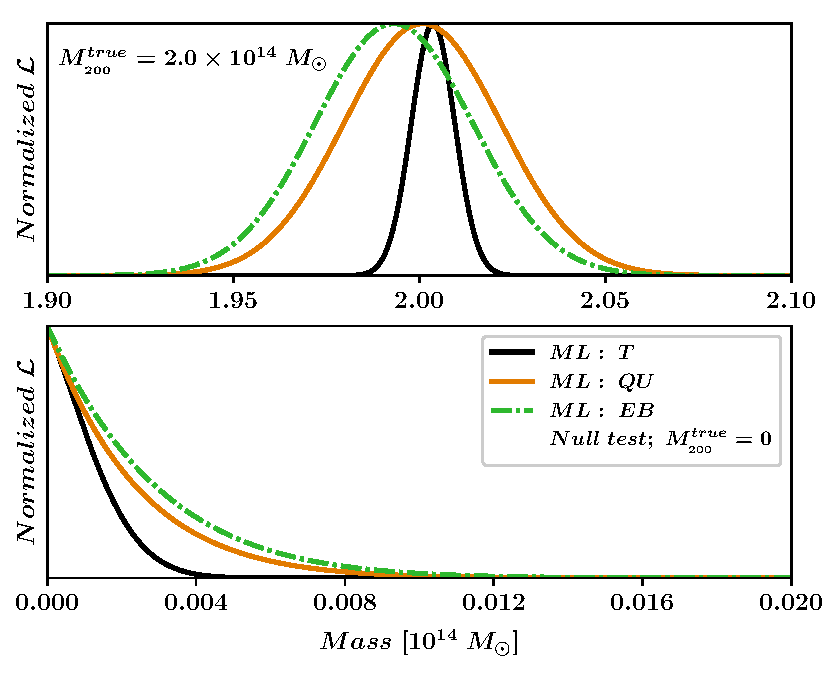
\includegraphics[width=\linewidth, keepaspectratio]{figs/fig0-eps-converted-to.pdf}
 \caption{In the top panel we show the combined likelihood of 100,000 clusters each at redshift of 0.7 and at mass of $2\times 10^{14} M_{\odot}$ for temperature and polarisation MLE estimators. The difference between QU and EB estimator isn't statistically significant. In the bottom panel we show the results of null test and as expected the likelihood peaks at zero for all three estimators}
 \end{figure}
 
 In the left panel of figure 2., we compare the performances of all three MLE estimators and the temperature QE estimator as function of experimental noise levels. 
 %Note that, no galactic or extra galactic foregrounds are added. 
 %All the fractional mass uncertainties are stated for 100,000 clusters each at a mass of $2\times 10^{14} M_{\odot}$ and at a redshift of 0.7.
 It is evident from the figure that in the absence of foregrounds, temperature outperforms polarisation above noise-level of 0.075 \ukam.
 So even for future CMB-S4 experiment temperature has to be the primary channel from pure SNR perspective.
 Only below noise-level of  0.075 \ukam, polarisation starts competing with temperature.
 As pointed out earlier, the lensing signal is directly proportional to the background CMB gradient, gradient in polarisation is 10$\times$ smaller than that of temperature as shown in ~\ref{fig:lensing_signal}. However, below noise-level of 0.075\ukam the CMB temperature background gradient acts as a source of noise. 
 
 Orange squares and green circles represent MLEs using polarisation QU maps and EB maps respectively. 
 As expected, there is no significant differences between their performance from a theoretical standpoint. 
 The apparent difference at higher experimental noise levels is not statistically significant.
 However, using QU maps simplifies the analysis as these modes are directly measured by the experiment and doesn't involve co-ordinate transformation ~\ref{eq:coord_trans}. In this chapter, I have considered only $QU_{MLE}$ polarisation estimator.
 
  
 Lastly, we compare the performance of temperature MLE (solid black triangles) and QE (orange solid squares). 
 QE is a first order approximation of MLE.
 %While both temperature MLE and QE perform equally well at higher noise levels, MLE has clear advantage over QE at low noise levels.
 At higher noise levels (low SNRs) the effect of higher order terms is negligible, hence no difference between the performance of MLE and QE estimators.
 However, at low noise levels (high SNRs) MLE outperforms QE. 
  Though not show here, there is no difference between polarisation MLE and QE for the range of the experimental noise we have considered.
  This is not surprising as polarisation lensing SNR is low for the considered noise levels.
 
 The effect of higher order terms can be recovered using an iterative version of QE as shown in \cite{Yoo and Zaldarriaga}.
 We find that MLEs performance is improves by a factor of 2 at noise level of 0.1\ukam  for our fiducial sample of 100,000 clusters each at  $M_{200} = 2 \times 10^{14}$ \msolar and redshift of 0.7. 
  
Both MLE and QE estimators share a common difficulty in regards with the assume cluster density profile.
This dependence shows up in different places in each estimators.
 \begin{itemize}
 \item In MLE as explained in ~\ref{sec_MLE} we fit the lensed CMB templates to the observed data. The lensed CMB templates are obtained by assuming a cluster density profile. 
 \item QE works by the exploiting the correlation between the background CMB gradient and lensing dipole to obtain lensing convergence profile. 
 We fit models to these lensing convergence profile to extract the mass of the cluster.
 
 \end{itemize}
There is no reason not take advantage of the improved performance of MLE over QE at low experimental noise levels. 
 \begin{figure}[t]
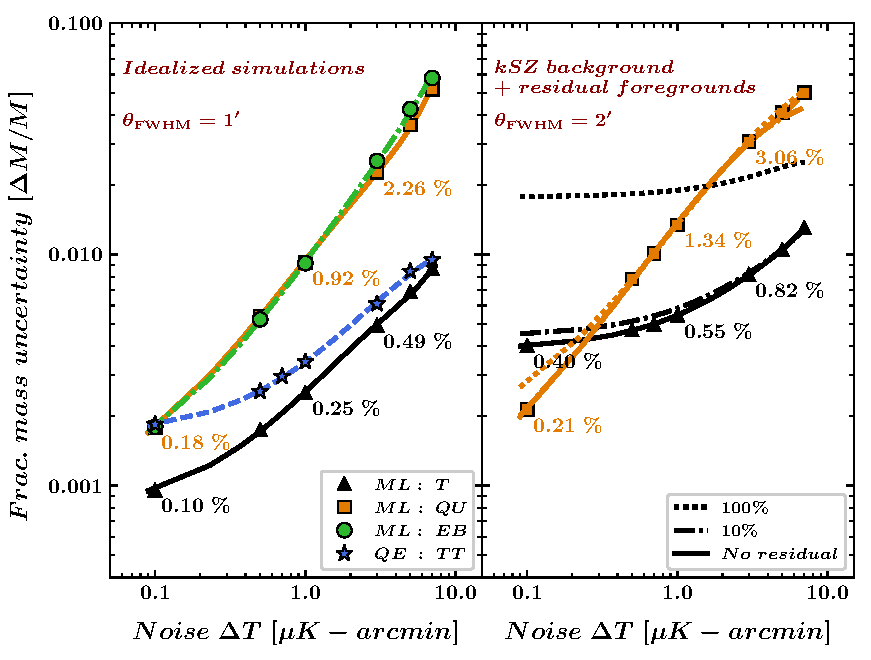
\includegraphics[]{figs/fig1-eps-converted-to.pdf}
 \caption{In the left we show the performance of different estimators for idealised simulations as function of experimental noise levels. We consider the effects of various foregrounds on the estimators in the right panel. All the curves are for a set of 100,000 clusters each at mass of $2\times 10^{14} M_{\odot}$ and at redshift of 0.7.}
 \end{figure}
   
   \subsection{Effects of extragalactic foregrounds on lensing analysis}
   In this section, we look into the effects of extragalactic foregrounds on lensing analysis. While galactic foreground also affect the lensing analysis, however, by using a combination of frequencies we can suppress galactic foregrounds. The bias due to some of the foregrounds such as cluster's own SZ effect etc., are reported in the next section. Here we are only concerned about the additional noise due to extra galactic foregrounds. The level of foregrounds is much higher in the temperature than in the polarisation channel, hence the effect of foregrounds is higher in temperature estimator than polarisation. We consider the impact of tSZ, kSZ, radio galaxies and dusty galaxies on the 150GHz channel.
   
   The impact of foregrounds on the performance of lensing estimators as function of experimental noise level is shown in fig. 2. 
   As expected foreground negligibly effects the polarisation channel (orange squares).
   For the temperature estimator the extragalactic foregrounds set an effective noise level of 5\ukam if not cleaned, this results in plateauing of 1.8\% in mass uncertainty (black dotted line). 
   Without any foreground cleaning polarisation QU estimator outperforms the temperature channel at 1.5 \ukam.
 However, we can exploit the frequency dependence of various extragalactic foregrounds to reduce the effect of foregrounds.
 While combining multiple frequency channels we assume that the beam size is 1\am  irrespective of the frequency to simplify the analysis. 
Using different spectral dependence of background CMB and tSZ we can completely eliminate the tSZ power.
 However, kSZ has the same spectral dependence as that of the CMB and hence cannot be eleminated. 
 The black solid triangles repersent the performance of temperature estimator 100\% kSZ and no tSZ, radio or dusty galaxies.
 The dashed solid line corresponds to 10 \% of radio and dusty galaxy power, 100\% of kSZ power and no tSZ power. 
 With 90\% cleaning of foreground, temperature estimator becomes the main channel for estimating lensing signal even for the proposed CMB-S4.
  There is only a fractional improvement in the performance above 90\% of cleaning. 
  It is important to note here that foreground cleaning enlarges the beam which is not taken into account here, which will degrade the mass uncertainties even further.
  
  To summarize, the extragalactic foreground almost have no effect on the performance of polarisation estimators. 
  On the other hand, temperature estimators will have effective noise floor of 5\ukam if foregrounds aren't taken into account. 
  As we will see in next in addition to increasing final mass uncertainties, some of these foregrounds will also acts sources of systematic bias.
  
  \section{Systematic bias checks}
  From figure 1, it is evident that we will achieve less than 1\% mass uncertainty for a CMB-S4 kind of experiment. 
  However, we need to account for all the systematic biases to claim our sub-percent mass measurements.
    In this section, we quantify various sources of systematics that could bias our final results.
    We examine the following sources:
    \begin{itemize}
    \item error in cluster center
    \item differences due to the cluster density profile
    \item other halos along the line of sight
    \item error in redshift
    \item cluster's tSZ effect
    \item cluster's kSZ effect
    \item dusty galaxies
    \end{itemize}
    The last three sources negligibly affect the polarisation estimators as they are only partially polarised. 
    Note that all these sources may effect polarisation and temperature estimators to different extents due to differences in the mode weighing between estimators.
     
 The baseline simulations for bias calculations include 1 \am Gaussian beam, experimental noise level of 1\ukam (which corresponds to a noise level of $\sqrt{2}$\ukam in polarisation) and no foreground unless otherwise stated.
  The amount of bias depends on experimental beam size, noise-level, and foregrounds as they define the weighing of different angular scales of MLE. 
  However, this section will roughly quantify the magnitude of bias and give a direction to pursue future work in CMB-cluster lensing to reduce the systematic uncertainties. 
   We report the systematic bias for a sample of 1,000,000 clusters each at a mass of $2 \times 10^{14}$ \msolar and each at a redshift of 0.7 (expect for redshift uncertainty case). The bias is calculated as follows:
   \begin{equation}
   b = \frac{M_{bias}}{M_{true}} - 1.
   \end{equation}
   where $M_{bias}$ is the final recovered mass when the source of bias of bias is included in the lensing analysis and $M_{true}$ is the input mass. 
   Error in the bias is obtained by calculating the scatter in 100 subsamples.
   
   We report the magnitude of bias for all the sources considered in table 1. 
 Other than errors in redshift, all other sources of bias should be considered carefully to achieve sub-percent uncertainty as claimed for CMB-S4 experiment. 
 Here we have not considered surveys specific systematics such as false detections, selection function, and projection effects or some form of bias in weighing the clusters.
 
 \subsection{Halos along the line of sight}
 In reality the final estimated mass also depends on other halos present along the line of sight and on the correlated halos. 
 If the effect due to these halos aren't taken into account then the final results will be biased high. 
 This is particularly a major concern for low mass haloes as they won't be detected by the survey/
 To quantify the effect of this bias we look into Flender et al simulation. 
 It is an N body cosmological simulation with 17 million objects; for cluster we random select a halo within a mass range of  $M_{200} \in$ [1.8, 2.2] $10^{14}$\msolar and redshift range of [0.6,0.8].
We simulate the CMB maps as explained earlier, however, instead of lensing the CMB with just the cluster convergence profile we lens it the all the convergence profiles which are within the 50\am of the cluster center. 
Analysis proceeds normally after this - these lensed CMB maps are convolved by Gaussian beam after which specified white experimental noise is added. 
As expected both polarisation and temperature estimators are biased high : 2.5 $\pm$ 0.3\% for temperature MLE and 6.3 $\pm$ 1.1\% for polarisation QU estimator.
We can reduce the bias by taking two halo term into account, however, that will include more nuisance parameters increasing the statistical uncertainty of the final results. 
Galaxy clusters are not isolated objects, they are generally found in large scale filaments. 
Also, clusters with ellipticity along the line of sight have higher tSZ increasing the probability of their detection. 
They are also likely to be found in filaments, resulting a high bias; however, the scope of finding the bias due to the large filaments is outside the scope this thesis. 
Its worth noting that in order to fully realise the potential of CMB-S4 in obtaining sub-percent mass uncertainties we need to work on systematics.
Accurate and reliable simulations of structure formation on large volumes is needed in order to handle this source of systematic error at the sub-percent level.

\subsection{Cluster mass profiles}
As mentioned earlier both QE and MLE assume a density profile, however, this may not be the true cluster profile. 
Any difference between the assumed mass profile and true cluster profile will bias the final results.
In all the above results we assumed clusters to follow NFW profile. 
However, studies have shown that for massive clusters the density profile deviates significantly from NFW at radius r $\ge$ 0.5 $R_{200}$. 
It is unknown whether these deviations will be larger or smaller for lower mass clusters.
In addition to this, a recent study has shown that for analysis involving stacked halos Einasto profile provides a better estimate.
Here we consider three density profiles in order to estimate the bias.
\begin{itemize}
\item A modified version of the NFW profile which drops off more rapidly with radius
\begin{eqnarray}
\kappa_{\rm NFW}^{mod}(x) =
\begin{cases}
    \kappa_{\rm NFW} &; x \le 0.75\theta_{_{200}}\\
    \kappa_{\rm NFW} \times m(i,j)&; 0.75\theta_{_{200}} < x \le 1.5\theta_{_{200}}\\
    0 &; otherwise
\label{eq_kappa_mod}
\end{cases}
\end{eqnarray}
where $m(i,j)$ is a Hanning 2D apodization kernel.
We create the 2D apodization kernel as $m(i,j) = m(i) \times m(j)$ with $m(i) = \frac{1}{2} \left[ 1 - cos\left(\frac{2\pi  (i-n/2) }{n} \right)\right]$, where i and j are pixel indices in the $n \times n$ map.
\item A change to the cuspiness of cluster core in the NFW profile, following \citet{king2001} 
\begin{eqnarray}
\kappa_{\rm NFW}^{sub}(x)  & =  &
\begin{cases}
    \kappa_{\rm NFW}\ + \sum\limits_{i=1}^{3} \kappa_{sub}^{i}&; x \le 1'\\
    \kappa_{\rm NFW} &; otherwise;
\label{eq_kappa_sub}
\end{cases}
\end{eqnarray}
\item The Einasto profile \citep{einasto1989}
\begin{eqnarray}
\rho(r)_{_{Ein}} & = &  \rho_{_{0}}\ exp\left( - \frac{2}{\alpha} \left[\left(\frac{r}{R_s} \right)^{\alpha} - 1\right]\right)
\label{eq_einasto_density}
\end{eqnarray}
with the shape parameter $\alpha = 0.18$ \citep{ludlow2013}. The convergence profile for this profile is obtained by inserting this into int\
o Eq.(\ref{eq_surface_denisty_los_integral}).
\end{itemize}
 
 In each of the three cases we lens CMB by the assumed cluster profile, however, we use NFW profile to calculate our model.
 Assuming wrong cluster profile will bias the results from -2.5\% to 3.8\% as shown in Table 1. 
 A similar study was done in optical weak-lensing analysis where they used NFW profile in the model and Einasto profile in the simulated data; they found a bias of -2 to 7 \% depending on the cluster mass. This level of bias is larger than the statistical mass uncertainties expected for the CMB-S4 experiment, and a significant challenge for upcoming experiments.
More work will be required to accurately measure the cluster mass profiles as a function of radius if we are to achieve the full potential of galaxy cluster cosmology. 

\subsection{Cluster miscentering}

Any difference between the true cluster center and the model will result in a bias.
 Misestimation of the cluster center even by a small amount results in underestimation of cluster mass as we loose some of the lensing signal.
To quantify the effect of miscentering, we draw an offset between from normal distribution N(0, $\sigma^{2}$) and lens the CMB with offseted clusters to obtain simulated data, however, model doesn't take the offset into account.
Fig 24 shows the bias in the final results as a function of offset for both temperature (orange squares) and polaristion estimators (black triangles).
As expected the bias increases with rms of the offset, the positive bias at very low offsets is not statistically significant.
Temperature estimator draws more information from smaller angular scales than the polarisation estimator, hence the bias in temperature estimator is more compared to the polarisation. Note that the here we haven't considered foregrounds, considering foreground would decrease the weightage of smaller angular scales. For survey with higher experimental noise, larger beams and foregrounds the bias will decrease.

 
The typical offset between the SZ-centroid and the X-ray or brightest central galaxy (BCG) is of the order of 0.5 \am.
From the figure, for 0.5 \am offset the mass is underestimated by 7.5 $\pm$ 0.3 \% for temperature estimator and 1.5 $\pm$ 1.3 \% for polarisation estimator. 
For a given constraint on the offset, a correction could be easily applied to eliminate the bias, however, that will result in a slight decrease of SNR.
Without considering the effect of foregrounds, we need to know the offset by 2\% (8\%) in order to achieve sub-uncertainty for future CMB-S4 survey.
However, adding foregrounds will reduce the weight of the information from smaller angular scales and lessen the requirement of how well the positional uncertainty must be known.
\begin{figure}[t]
\centering
%\hspace{-2mm}                                                                                                                               
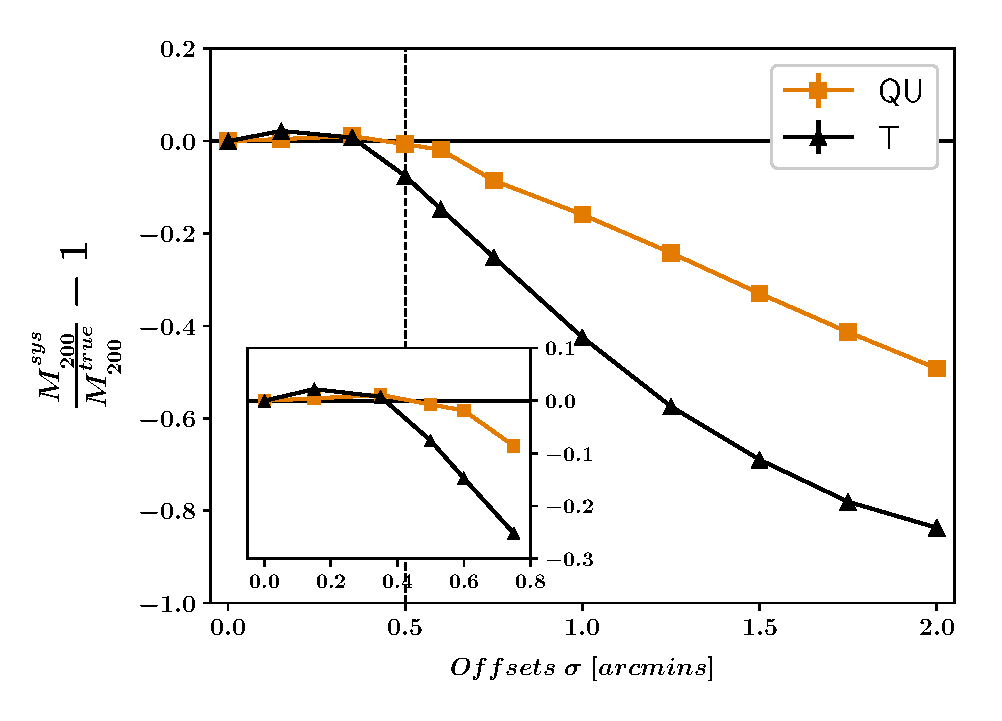
\includegraphics[width=0.85\textwidth, height=0.65\textwidth,clip=]{figs/fig2_v2.eps}
\caption{The low mass bias due to the positional offsets between SZ determined centroid and the true cluster center  for the $T_{\rm ML}$ (b\
lack triangles) and $QU_{\rm ML}$ (orange squares) estimators. The typical positional offset of $0.5'$ \citep{song2012} is marked with the v\
ertical dashed line. The error bars are derived using estimates gathered by repeating the test 100 times.}
\label{fig_sys_bias_cluster_offsets}
\vspace*{2mm}
\end{figure}


 \subsection{Redshift Bias}
CMB-cluster lensing can be used to calibrate the mass scaling relations of SZ surveys (SPT-3G, AdVACT, Simons Observatory etc.,), optical surveys (LSST, DES etc.,), and X-ray surveys (eRosita etc.,). These surveys are expected to return tens to hundreds of thousands of clusters, however, obtaining spectroscopic redshift for each cluster is not feasible.  
On the other hand, we can have red squence redshifts up to an higher redshift threshold and a redshift lower limit for clusters at even higher redshifts. 
The current state of the art for red sequence redshifts can be seen in the  DES \texttt{redMaPPer} catalog, where the \emph{photo-z} errors are $\sigma_{z} = 0.01 (1+z)$ for $z \le 0.7$ and $\sigma_{z} = 0.02 (1+z)$ for $z \sim 0.9$ \citep{rykoff2016}. The mass bias is estimated by considering a redshift scatter for individual clusters. We conservatively take the redshift errors to be
\begin{equation}\nonumber
\sigma_z = \left\{
\begin{array}{l}
    0.02 (1+z);  ~~z < 1 \\
    0.06 (1+z);  ~~z > 1
  \end{array}\right.
\end{equation}

We create mock lensed CMB maps using the true redshifts $z\in[0.5, 1, 1.5, 2]$ for the cluster. However, the `measured' redshift, $z + \sigma_{z}$, for each cluster is used to construct the pixel-pixel covariance matrix. The masses are then fit using this incorrect covariance mat\
rix, and the fractional bias determined.                                                                        
The case that should have the largest bias, $z=2$, is listed in Table~\ref{tab_sys_bias}. We do not detect a mass bias at any redshift. 
 
\subsection{kinematic SZ signal}
CMB photons get doppler shifted due to the relative motion of the galaxy cluster with respect to the CMB rest frame, this is know as kinematic Sunyaev - Zel'dovich effect (kSZ).
While kSZ is an order magnitude smaller than tSZ, unlike tSZ effect, kSZ effect has the same spectral dependence as that of CMB. 
We cannot combine multiple frequency channels to eliminate kSZ effect. 
Instead we can use polarisation estimator as, it is only partially polarised.

To quantify the kSZ bias, we consider the publicly available kSZ maps and halo catalog from Flender et al simulations.
These are full sky simulations in healpix pixelisation scheme with nside of 8192 correpsponding to 0.42 arcminute resolution.
Within a mass range of $M_{200} \in [1.8 \times 10^{14},2.2 \times 10^{14}]$ $M_{\odot}$ and redshift $\in$ [0.6,0.8] the catalog has 20,000 halos. 
For each cluster in the simulated data we randomly pick 50\am $\times$ 50\am cutout centered around the halo, smooth it with experimental Gaussian beam of FWHM = 1\am and add it to the lensed cluster cutout. 
Final results are significantly biased if the the kSZ effect is not taken into account while modeling the pixel-pixel covariance matrix: we obtain a low bias of 41\%.
We get similar large bias levels when we used an analytic modelling for the cluster kSZ signal instead of extracting them from N-body simulations. Modelling the optical depth of the clusters using the Battaglia \cite{nickb2016} profile and drawing the cluster velocities from a normal distribution $N(0, \sigma^{2})$ with scatter $\sigma = 350\ km/s$, we obtained a 32\% bias in the recovered lensing mass.
  
 If we take effect of kSZ while modeling the pixel-pixel covariance matrix then as expected we eliminate the bias. 
 However, we don't exactly know the kSZ effect of a single cluster. According to current estimates the uncertainty in kSZ prediction is 20\% for a single galaxy cluster. 
 The reason for the uncertainty is the complex cluster baryonic physics which is not very well understood. 
 To determine the bias that would result due to the uncertainty in kSZ effect, we included 20\% uncertainty in the modeling the pixel-pixel covariance matrix. 
 This results in a low bias of 7.5 $\pm $ 0.4 \%, bias can either be low or high depending on underestimation or overestimation of kSZ.
 Interpolating linearly between the kSZ uncertainty and the bias, we find that 2-3\% uncertainty in kSZ would lead to sub-percent bias. 
 Given the current uncertainties in kSZ estimation, it acts as a serious obstacle in using CMB-cluster lensing for future CMB surveys. 
 
 \subsection{Thermal Sunayev-Zel'dovich effect}
 
Here we give a brief review of Thermal Sunayev-Zel'dovich (tSZ) effect and is explained in detail in the next chapter.
CMB photons while passing through galaxy cluster are inverse compton scattered of high energetic electrons present in cluster's hot intra cluster medium.
This results in excess of photons at higher frequency and deficit of photons at lower frequency, this is known as tSZ effect.
tSZ effect is an order of magnitude greater than lensing signal and will induce significant statistical and systematic uncertainties if not taken into account.
In the next two chapters we discuss in detail the methods through which we eliminate the tSZ bias in QE estimator.
Here, we quantify the tSZ bias in the MLE and discuss the methods that can be used to reduce the bias.
We consider two different approaches:
\begin{itemize}
\item use frequency channels to eliminate the tSZ
\item model the tSZ effect in the pixel-pixel covariance matrix
\end{itemize}
In an ideal world both of these approaches should completely eliminate the bias, however, due imperfect knowledge in the instrument calibration or the model will result in a bias. 
To evaluate the performance of each approach,  we use Compton $y$ maps produced on a $5^{\circ} \times 5^{\circ}$ box at resolution $2.'5$ from the smoothed-particle hydrodynamics (SPH) simulations of  \citet{mccarthy2013}.
Neglecting relativistic corrections, we convert the Compton $y$ maps into tSZ maps by
\begin{eqnarray}
\Delta T = y T_{\rm CMB} \left[x \left(\frac{e^{x/2} + e^{-x/2}}{e^{x/2} - e^{-x/2}}  \right)\right]
\end{eqnarray} where $x = \frac{h\nu}{k_{\rm B}T_{\rm CMB}}$, $\nu$ is the frequency in GHz, $T_{\rm CMB} = 2.73\ K$, $k$ is the Boltzmann constant, and $h$ is the Planck constant.

\subsection{tSZ frequency cleaning}
 Using the spectral dependence of tSZ we can eliminate it by using CMB maps observed at different frequency channels.
 In this chapter we assume the CMB is observed at 90 GHz and 150 GHz channels with Gaussian beam of FWHM 1.7\am and 1\am respectively.
 The tSZ amplitude at 90 GHz is 1.67 times that of 150 GHz.
 tSZ free map is obtained as follows:
 \begin{equation}
\widetilde{T}(\hat{\textbf{n}})  =  \frac{1.67\widetilde{T}_{{150}}(\hat{\textbf{n}}) - T_{{90}}(\hat{\textbf{n}})}{f-1}
\end{equation}
where
\begin{equation}
\widetilde{T}_{{150}}(\hat{\textbf{n}})  =  T(\hat{\textbf{n}})_{{150}} \ast \frac{B_{{90}}(\hat{\textbf{n}})}{B_{{150}}(\hat{\textbf{n}})},
\label{eq_smooth}
\end{equation}
 f is 1.67. It is important to note that 150 GHz has to smoothed with 90 GHz beam using \ref{eq_smooth} before subtracting out tSZ.
  For the analysis we have also assumed that the experimental noise level in both 90 and 150 GHz channels to be 1 \ukam. 
  Under these assumptions using tSZ free map will eliminate the bias (b = 0.0 $\pm$ 0.7), however, it will degrade the final SNR by a factor of three.
  In practice, it is unlikely to obtain a precise value of factor 'f' due the uncertainties in frequency band widths or errors in relative calibration of frequency bands.
  To evaluate the bias in the final results due to the uncertainties in the factor `f', we use simulations. 
  We assume an uncertainty of 1\% in f, which is overly conservative for future CMB surveys but comparable to that of current surveys.
 An error in f will result in leakage of tSZ in the final tSZ free maps and will bias the results.
 For 1\% uncertainty in `f' we find the final results to be biased low by -6.3 $\pm$ 0.7 percent. 
 The bias can shift depending on whether the SZ leakage is over estimated or under estimated.
  
tSZ has no power at 217 GHz and one might consider of using 217 GHz frequency channel instead of creating tSZ free maps. 
However, the power dusty galaxies are increase significantly with frequency.
So, the foreground power in 217 GHz channel is much more than 90 or 150 GHz channels. 
In addition to that, we should also take into account the contamination due to the correlation between the tSZ and cosmic infrared background due to these dusty galaxies.
 Current estimates find the correlation co-efficient to be $0.113^{+0.057}_{-0.054}$; estimating the tSZ-CIB signal at 220 GHz would yeild a signal nearly three quarters of the tSZ signal at 150 GHz. 
 In order to use 217 GHz channel, more work needs to be done in constraining the tSZ-CIB correlation.
 
 \subsection{tSZ fitting}
 Instead of removing the tSZ signal, one can include it in the pixel-pixel covariance matrix.
Following \S\ref{sec_kSZ_bias}, we calculate the expected tSZ contribution using SPH simulations from \citet{mccarthy2013}.
As would be expected, the bias is consistent with zero for perfect knowledge of the tSZ signal (b = $1.0 \pm 0.6\%$).
However, this bias increases quickly if the tSZ contribution is mis-estimated.
Analogously to the tSZ cleaning case, we would expect percent-level errors to lead to significant (order 6\%) biases.
Given that the current uncertainties in modeling the tSZ signal from galaxy clusters are more than an order of magnitude larger, it will be extremely challenging to achieve the sub-percent precision necessary to make this approach viable.
Another way is to tSZ model out of the 150 GHz channel.
 While this method doesn't degrade the SNR unlike the frequency cleaning, however, imperfect knowledge in theoretical modelling will result in a bias.
 
 
 \subsection{Dusty galaxies in the cluster and other foregrounds}
\label{sec_DG_sys_bias}


Galaxy clusters are known to host overdensities of dusty galaxies, with several papers measuring the resulting tSZ-CIB correlation \citep{actdunkley2013, george2015, PLANCKTSZCIB2016}.
We describe our modeling of these DG overdensities\footnote{For implementation reasons, in this section, we include all foregrounds mentioned in the Appendix \ref{sec_appendix}, even ones that are not cor\
related with the cluster itself, such as radio galaxies.} in the Appendix \ref{sec_appendix_extragal}.
If ignored, the tSZ-CIB correlation may substantially bias the recovered masses from temperature estimators, especially at higher frequencies.
The emission from dusty galaxies rises sharply with frequency, by an order of magnitude in $\mu K^2_{\rm CMB}$ from 90 to 150\,GHz and again from 150 to 220\,GHz.
Polarization estimators (at least at 150\,GHz and lower frequencies) are essentially unaffected due to the lower polarization fraction  of dusty galaxies (expected to be less than 4\% \citep{seiffert2007,sptpol_delensing_2017}).
The tSZ-CIB correlated power could be handled analogously to either the tSZ fitting or cleaning approaches in \S\ref{subsec:tszbias}.
However, a multi-frequency cleaning scheme will be less effective than for the tSZ effect since the spectral dependence of thermal dust emission varies between individual galaxies.
Here we look only at bias for the fitting approach where the extra pixel-pixel covariance due to the clustered dusty galaxies is folded into the likelihood.
The recovered mass is somewhat low: $b=4.5 \pm 1.7\%$.
The existence of a bias (higher than $2\sigma$) is slightly surprising since one would expect zero bias in the perfect information limit, and the significance is low enough that it may be a statistical fluke.
The dramatic increase in the uncertainty -- from 0.25\% to 1.7\% -- reflects the plateauing of the dotted line in right panel of Fig.~\ref{fig_delM_M_1000_clusters_T_QU_EB_ideal_FG}.
Unsubtracted foreground power effectively sets a lower bound on the instrumental noise.

\section{A look into the future}
\label{sec_forecast}

\begin{figure}
\centering
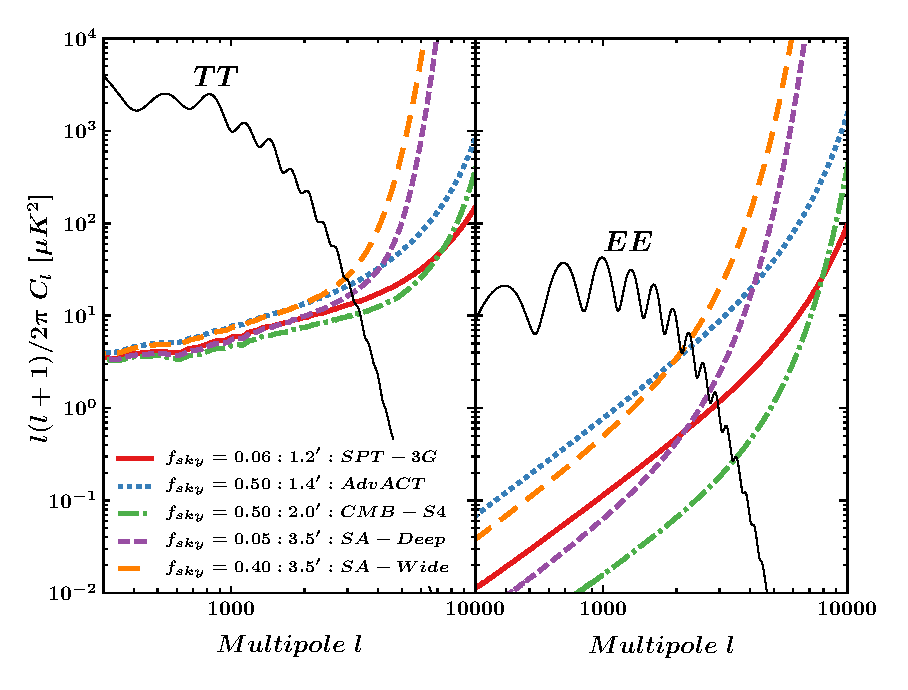
\includegraphics[width=1.\textwidth, height=0.68\textwidth,clip=]{figs/fig3.eps}
\caption{The expected residual foreground and noise power spectrum for the future CMB experiments.
The 90, 150, and 220 GHz channels have been combined using a constrained ILC technique to remove the tSZ effect while minimizing other extragalactic foregrounds and instrumental power.
The left and the right panels correspond to temperature and polarization respectively.
The plateauing of the residual temperature spectrum reflects the limited foreground removal possible with three frequency channels.
Specifications about each experiment are listed in Table \ref{tab_forecast_future_CMBexp}.}
\label{fig_ILC_res}
\end{figure}

In this final section we forecast the cluster mass uncertainties from CMB-cluster lensing for the AdvACT, Simons Array, and SPT-3G experiments, which we will collectively refer to as the Stage III experiments, \
and also for the proposed CMB-S4 experiment.
In addition to presenting the mass uncertainties for fiducial versions of these experiments, we examine how the mass uncertainty would change as a function of the beam size and map noise levels.
This information can be used to evaluate design tradeoffs while planning the CMB-S4 experiment.

\subsection{Expected lensing mass uncertainties for future CMB experiments}
\label{subsec:cmbs3s4}

We expect the next generation of CMB experiments, which will have substantially more detectors and a concomitant reduction in map noise levels, to dramatically improve the cluster mass calibration possible from\
 CMB-cluster lensing.
The experimental configuration of all the experiments considered is given in Table \ref{tab_forecast_future_CMBexp}.
Three options for telescope size (and therefore beam sizes) are listed for the proposed CMB-S4 experiment.
While current results have mass uncertainties of order $\ge 20$\% \citep{baxter2015,act_cmass2015,planckXXIV2015}, we expect Stage III experiments to reach 3\% and CMB-S4 to approach 1\%.

There are two reasons for the improvements.
First, with more detectors comes lower map noise levels (and larger survey areas).
The deepest current experiments reach approximately $5\,\mu$K-arcmin in temperature; the Stage III surveys  (AdvACT \citep{advact_2016};  Simons Array \citep{PB2_2016}, and SPT-3G \citep{benson2015_3g}) forecas\
t a few $\mu$K-arcmin; and projections for CMB-S4 are $\sim$\,1\,$\mu$K-arcmin.
Lower noise improves the lensing significance on any individual galaxy cluster.
Second, lower noise levels and larger survey areas translate into substantially more galaxy clusters.
Current ground-based SZ cluster catalogs have fewer than 1000 clusters \citep{ACTSZ2013, bleem2015}, but SPT-3G is forecast to find 8000 clusters \citep{benson2015_3g}, AdvACT 10,000 clusters \citep{advact_2016} and we assume ad-hoc that CMB-S4 will find 100,000 clusters.
In addition to the internally discovered clusters, optical surveys like DES \citep{rykoff2016}, and in the future LSST \citep{lsst_science_book} and Euclid \citep{euclid_science_book}, will yield extremely larg\
e numbers of galaxy clusters within the CMB survey regions, as will the X-ray satellite eROSITA \citep{erosita_science_book}.
This method is perfectly suited to determining the mass calibration for these external cluster catalogs as well.

\begin{figure*}[tbh]
\centering
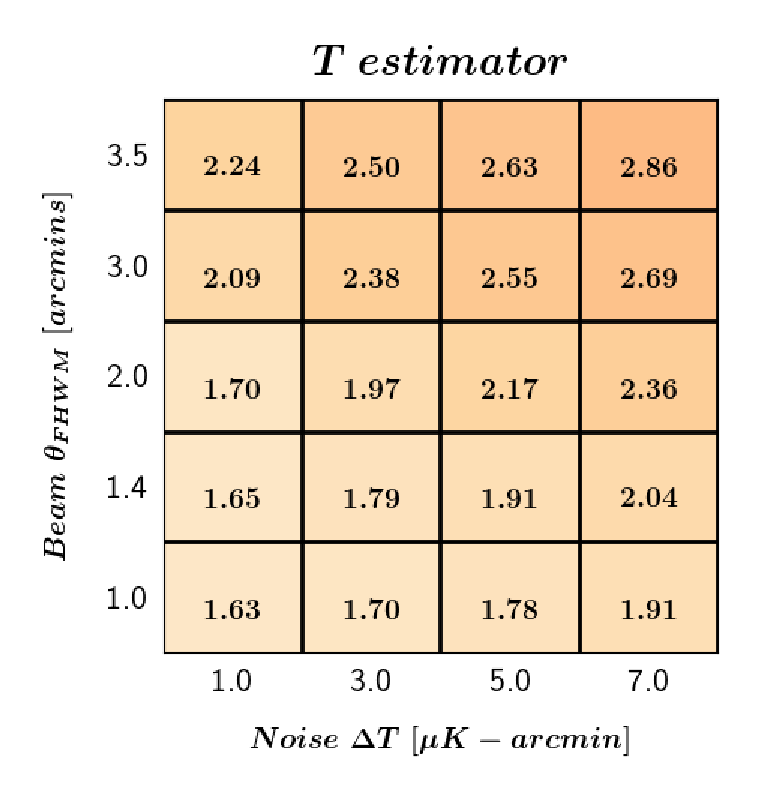
\includegraphics[width=0.46\textwidth, height=0.5\textwidth,clip=]{figs/fig4.eps}
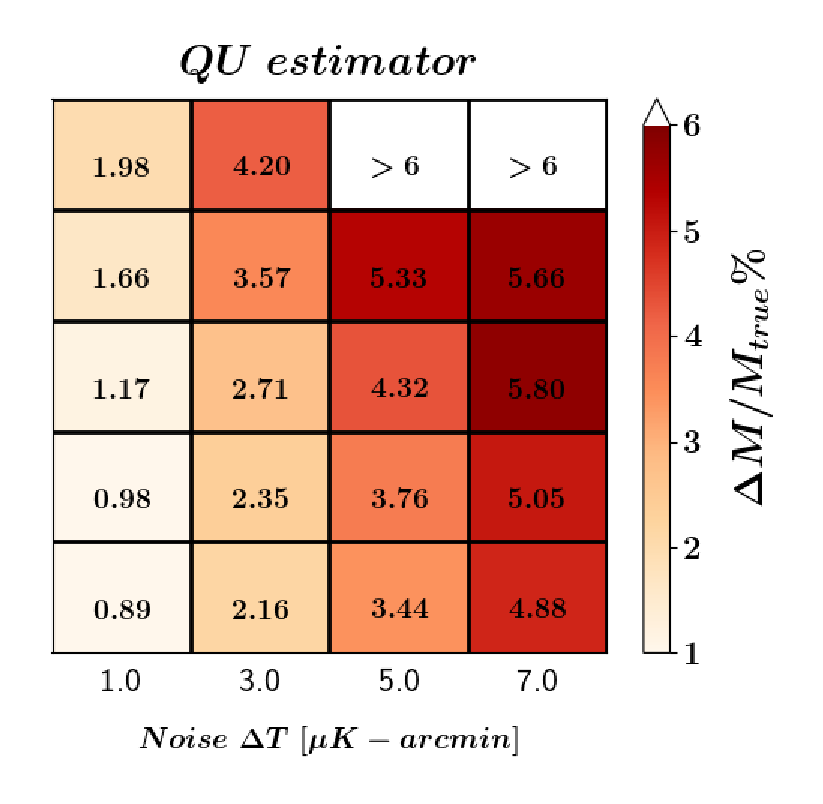
\includegraphics[width=0.5\textwidth, height=0.5\textwidth,clip=]{figs/fig5.eps}
\caption{The performance of the polarization MLE is very sensitive both to the angular resolution and map noise level of an experiment; the gains for the temperature MLE are much smaller. The numbers correspond\
 to the CMB-cluster lensing mass uncertainty (in percent) of the cluster sample containing 100,000 clusters after the addition of foregrounds (dotted lines in right panel of Fig. \ref{fig_delM_M_1000_clusters_T_QU_EB_ideal_FG}).
Improving the beam from $3.'5$ to $1'$ enhances the SNR by a factor of two for the CMB-S4 noise levels.
The saturation of $T_{\rm ML}$ is due to the larger impact of foregrounds on the temperature maps. }
\label{fig_beam_dependency_T_QU}
\end{figure*}

To provide realistic estimates of the mass uncertainties, we perform a constrained internal linear combination (ILC) of data from 90, 150, and 220 GHz channels based on the \texttt{SMICA} (Spectral Matching Ind\
ependent Component Analysis) algorithm \citep{smicacardoso, PLANCKCOMPSEP2014} to eliminate the tSZ signal from the temperature data and minimize the residual power in other extragalactic foregrounds and instru\
mental noise in both temperature and polarization.
The resulting power spectra of the instrumental noise and residual foregrounds for different CMB experiments are shown in Fig.~\ref{fig_ILC_res}.
At $\ell \le 2000$, the temperature curves are dominated by residual foreground power as three frequency bands are insufficient to completely eliminate the foreground power in the assumed model (see Appendix).
As a result, the temperature noise curves  converge at $\ell \le 2000$ despite the very different noise levels of the  experiments.
During this process, we convolve the 90 and 220 GHz spectra by the ratio of 150 GHz beam and their native beams, so that the final effective beam size matches 150 GHz.

The expected performance of each  experiment is given in Table \ref{tab_forecast_future_CMBexp}.
One significant uncertainty is the number of clusters to assume for each experiment.
As accurately modeling the survey selections functions for SZ, optical, and X-ray surveys is beyond the scope of this work, we make the simplifying assumption that all Stage III experiments will have 10,000 clu\
sters and the CMB-S4 experiment will have 100,000 clusters.
%This is of order the number expected to be discovered through the tSZ effect by the SPT-3G (8000 clusters; \citet{benson2015_3g}) or AdvACT (10,000 clusters; \citet{advact_2016}), but likely an over-estimate f\
or the Simons Array due to its larger 3.5$^\prime$ beam size.                                                                                                                                                      
This is of order the number expected to be discovered through the tSZ effect by the SPT-3G or AdvACT (see above), but likely an over-estimate for the Simons Array due to its larger 3.5$^\prime$ beam size.
On the other hand, the experimental beam size is irrelevant when predicting the size of cluster samples from optical or X-ray surveys that overlap with the CMB surveys.
The DES or LSST surveys should provide samples with more than 50,000 clusters for all of the Stage III CMB experiments \citep{rykoff2016, lsst_science_book}.
Given a specific sample size, the mass uncertainty can be obtained by rescaling the numbers provided in Table \ref{tab_forecast_future_CMBexp} by $\sqrt{\frac{N_{sample}}{N_{clus}}}$.

Even considering concerns about potential biases from astrophysical signals, the temperature channel will be extremely important for the cluster mass estimates from the Stage III CMB experiments.% (AdvACT, Simo\
ns Array, SPT-3G).
 The mass uncertainty on the fiducial 10,000 cluster sample  is similar in temperature from all three experiments, with a range from 3.3\% (SPT-3G) to 5.9\% (the Simons Array wide survey). These uncertainties ar\
e as large as the likely systematic uncertainties, and the statistical uncertainties on polarization are higher by a factor of two or more. As an example of scaling the results with sample size, we replace the \
fiducial sample size by the expected number counts for SZ-discovered clusters with SPT-3G (8000) and optically detected clusters from the DES (50,000). SPT-3G would achieve a 3.6\% mass uncertainty with a sampl\
e of 8000 SZ-selected clusters and a 1.5\% uncertainty on a sample of 50,000 optically-selected clusters. The shallow portions of the Simons Array or AdvACT surveys cannot contribute much for the polarization e\
stimator; lower noise levels are essential. The polarization estimator can be within a factor of two for the deep surveys of the Simons Array or SPT-3G. For instance, the polarization estimator for SPT-3G on 80\
00 clusters yields a 6.8\% mass calibration, to be compared to the 3.6\% mass calibration from temperature (ignoring systematic uncertainties).


The lower level of systematic uncertainty for polarization comes into play for the CMB-S4 experiment. First, for the extremely low noise levels of CMB-S4, the performance of the temperature and polarization cha\
nnels is nearly identical (0.95\% vs.~0.98\%) for an instrument with $2'$ beam resolution. Second, the magnitude of the temperature-only systematic errors (primarily from the SZ effect) is now several times lar\
ger than the raw statistical uncertainties, and would dominate the temperature error budget. We can expect cluster mass calibrations from CMB-S4's polarization data at the 1\% level.

The mass calibration forecasts in  Table \ref{tab_forecast_future_CMBexp} are highly complementary  to and competitive with the masses obtained by stacking optical weak lensing measurements. For example, LSST h\
opes to achieve a mass uncertainty of 1\% by stacking few thousands of clusters at redshifts $z < 0.5$ \citep{lsst_science_book}. At high redshifts, since the number density of background galaxies decrease rapi\
dly, the constraints from optical lensing measurements tend to weaken. Calibrating the high redshift end of the mass function is the true power of CMB-cluster lensing which will allow us to place important cons\
traints on the redshift evolution of mass-observable scaling relations out to high redshifts $z \ge 1.5$.
		 
%  -------  Data Analysis  -------  
\setcounter{chapter}{2} %3
		 \chapter{modified Quadratic Estimator}
\label{ch:analysis}
\section*{Overview}\label{ovr}
In this chapter we discuss modified Quadratic Estimator which we have developed to eliminate the bias due thermal Sunyaev Zel'dovich (SZ) effect. 
We give a brief review thermal Sunayev-Zel'dovich effect (refer \pending{citations} for a detailed review)and its effect on cluster lensing in the \S\ref{tsz}.
Then we discuss the modifications of the QE to remove SZ bias in \S\ref{sec_method}.
 Later we explain the SPTpol and DES data sets in \S\ref{sec_data} and results in \S\ref{sec_results}
Finally we conclude in \S\ref{sec_conclusions}.
%We explain the constraints on mass-richness scaling relation obtained using the above data. 


\section{Thermal Sunayev-Zel'dovich effect}\label{tsz}

 Cosmic microwave background (CMB) photons gets inverse Thompson scattered off the high energetic electrons present in the intra cluster medium of a galaxy cluster, resulting in a deficiency of photons at lower frequency and excess of photons at higher frequency. 
 This phenomena is called thermal Sunayev-Zel'dovich effect (SZ). 
 SZ is a small effect and to illustrate it we have shown CMB spectral distortion for a fictional galaxy cluster of mass 1000 times more that of a typical galaxy cluster in Fig ~\ref{ned_plot}.
 The solid black curve represents the intensity of CMB as a function of frequency before its interaction with hot intracluster medium; solid blue represents the same after its interaction.
 As shown in the Fig.~\ref{ned_plot}, SZ decreases the intensity of CMB below a frequency of ~ 220 \,GHz and increases at higher frequencies. 
   
The fractional change in temperature is given by 
\begin{equation}
\label{eq:sz_eqn}
\frac{\Delta T_{SZ}}{T_{CMB}} = f(x) y = f(x) \int n_{e} \frac{k_{B}T_{e}}{m_{e}c^{2}} \sigma_{T} dl
\end{equation}
where $y$ is Compton $y$-parameter, $n_{e}$ is the electron number density, $m_{e}$ is the electron rest mass, $c$ is the speed of light,  $T_{e}$ is the electron temperature, $\sigma_{T}$ is the Thompson cross-section, and f(x) is the dimensionless frequency given by
\begin{equation}
f(x) = (x\frac{e^{x}+1}{e^{x}-1} -4)(1 + \delta_{SZE}(x,T_{e}))
\end{equation} 
where $\delta_{SZE}(x,T_{e})$ is the relativistic correction to the frequency dependence.
\begin{figure}
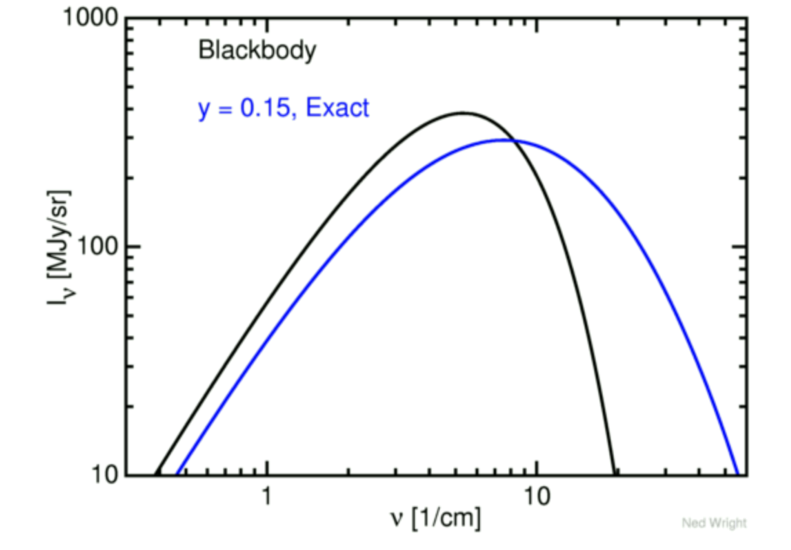
\includegraphics[width=\linewidth]{figs/tSZ_effect_Ned.png}
\label{ned_plot}
\caption{The plot shows the intensity of CMB as function of frequency before (black) and after (blue) it passes through a cluster. }
\end{figure}

As can be seen in \ref{eq:sz_eqn} SZ effect is independent of redshift and has potential to high redshift clusters, where the cluster abundance critically depends on underlying Cosmology.
CMB surveys use SZ effect to detect galaxy clusters; %, galaxy clusters appears as blue blob at frequencies lesser than 220 \, GHz.
Fig. \ref{fig:clus_in_cmb} shows a galaxy cluster of mass $M_{200m}\footnote{$M_{200m}$ is defined as the mass of the cluster within a radius $R_{200}$, within which the cluster density is 200 times the critical density of the Universe at cluster redshift} = 5*10^{14} M_{\odot}$ as seen by CMB survey. 
\begin{figure}
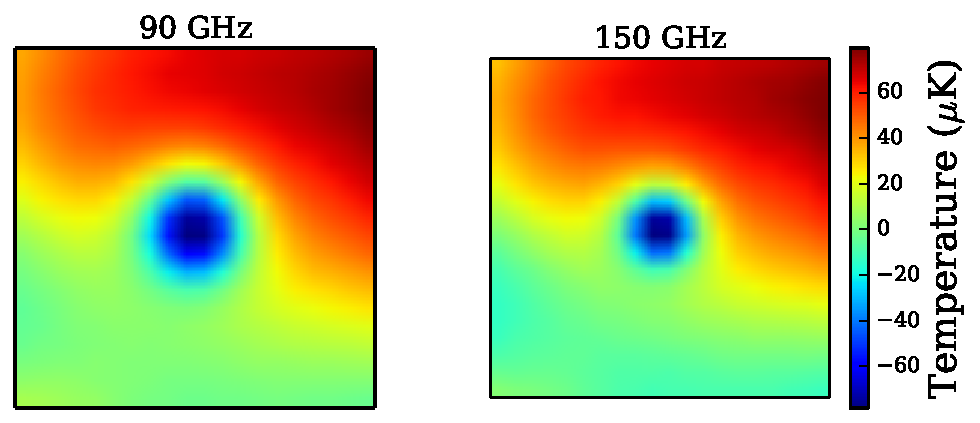
\includegraphics[width=\linewidth]{figs/clus_in_cmb}
\label{fig:clus_in_cmb}
\caption{Galaxy cluster of mass $M_{200m} = 5*10^{14} M_{\odot}$ as seen in a CMB survey with following specifications : 1.\arcmin7  beam at 90 \,GHz (left panel) and 1\arcmin  beam at 150 \, GHz (right panel). }
\end{figure}
 
 Though SZ is small spectral effect, it is still much higher than the lensing signal. 
 It is an order of magnitude greater than the lensing signal and hence induces a significant systematic and statistical uncertainty if not taken into account. 
 Fig ~\ref{fig:SZ_effect} shows the effect of SZ on the lensing convergence profile. 
 In the left panel of figure we show the stacked lensing convergence profile of 1000 clusters each with a mass of $4*10^{14}$ $M_{\odot}$ and an experimental noise of 1\ukam with no SZ and on the right panel is with the SZ.  
 As can be inferred from the plot, presence of SZ induces a blue blob in the center and hence resulting in a negative bias.
 \begin{figure}
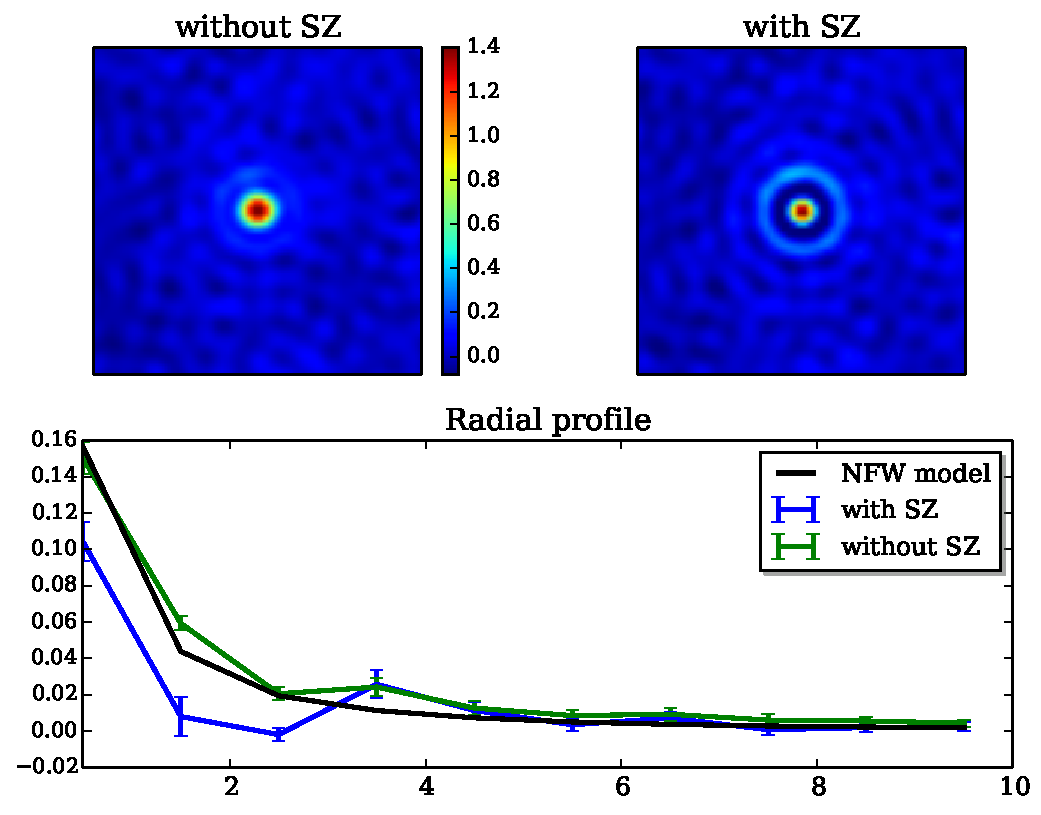
\includegraphics[width=\linewidth]{figs/tSZ_effect_on_lensing.pdf}
\caption{Effect of SZ on lensing convergence profile. On the top panel we show the lensing convergence profile for a stack of 1000 cluster each at a mass of $M_{200m}= 2*10^{14}  M_{\odot}$ and a redshift of $z = 0.7$ with experimental white noise level of $3\ukarcmin$; left panel is without SZ and right panel is with SZ. On the bottom panel we have radial profile of the same in solid blue (without SZ) and green (with SZ) curves; black curve is the radial profile of the input NFW profile. }
\label{fig:SZ_effect}
\end{figure}



\section{Methods}
\label{sec_method}
\section{Quadratic Estimator}
%Quadratic Estimator is based on two approximations: gradient approximation and linearization in convergence.

Typical size of galaxy cluster is of the order of few arc minutes. 
Primordial CMB doesn't have power at such small scales due to diffusion damping \cite{Silk} and can be approximated as a gradient. 
Lensing due to galaxy cluster induces a dipole kind of structure oriented along the direction of background gradient with hot and cold spots swapped.
For a given cluster mass and redshift, the magnitude of this dipole scales linearly with the magnitude of the CMB gradient.
This correlation between the unlensed CMB gradient and lensing signal is known as the gradient approximation and is equivalent to
\begin{equation}
T (\hat{n})\approx \tilde{T}+ \nabla T . \vec{\alpha}(\hat{\textbf{n}})
\end{equation}
Below we provide the mathematical formalism for temperature quadratic estimator and it generalises for polarisation.

 Under the gradient approximation, we construct an estimator of lensing convergence by multiplying the lensing map and the gradient map.
The gradient approximation doesn't hold for all Fourier modes, only for the modes which are correlated by reconstruction.
We filter maps in the Fourier space to isolate modes for which the gradient approximation is valid.
%\begin{equation}
% \hat{k_{l}} = -A_{l} \int d^{2} \hat{n} e^{i\hat{n}.l} Re{\nabla .[G(\hat{n}) L^{*}(\hat{n})]}
 %\end{equation}
 We obtain gradient and lensing maps as follows,
 % $G(\hat{n})$, $L(\hat{n})$ are filtered gradient and lensing maps respectively, $A_{l}$ is the normalisation parameter.
 % We obtain $G(\hat{n})$, $L(\hat{n})$ from the observed temperature map as follows
  \begin{eqnarray}
  L(\hat{n}) = \int \frac{d^{2}l}{(2\pi)^{2}} e^{il .\hat{n}} W^{T}_{l} T_{l}\\
  G(\hat{n}) = \nabla (\int\frac{d^{2}l}{(2\pi)^{2}} e^{il .\hat{n}} W^{TT}_{l} T_{l}   )
  \end{eqnarray}
  where $G(\hat{n})$, $L(\hat{n})$ are filtered gradient and lensing maps and $T_{l}$ is the observed temperature map in Fourier space.  
 Fourier filters $W^{T}_{l}$ and $W^{TT}_{l}$ are given by 
 \begin{eqnarray}
 W^{T}_{l} = (C^{TT}_{l} + N^{TT}_{l})^{-1}\\
 W^{TT}_{l} =  \widetilde{C}^{TT}_{l}(C^{TT}_{l} + N^{TT}_{l})^{-1}
 \end{eqnarray}
 where  $\widetilde{C}^{TT}_{l}$,$C^{TT}_{l} $  is the unlensed and large scale structure lensed CMB power spectrum obtained from \texttt{CAMB}, $ N^{TT}_{l}$ is the experimental noise power spectrum.
 With filtered gradient and lensing maps in hand we can write down the expression for lensing convergence profile as 
 \begin{equation}
 \hat{k_{l}} = -A_{l} \int d^{2} \hat{n} e^{i\hat{n}.l} Re{\nabla .[G(\hat{n}) L^{*}(\hat{n})]}
 \end{equation}
 where $A_{l}$ is the normalisation parameter given by
 \begin{equation}
 \frac{1}{A_{l}} = \frac{2}{l^{2}} \int \frac{d^{2}l_{1}}{4\pi^{2}} (l.l_{1}) W^{TT}_{l} W^{T}_{l} (\tilde{C}^{TT}_{l_{1}}(l.l_{1}) + \tilde{C}^{TT}_{l_{2}}(l.l_{2}))
 \end{equation}
 where $l = l_{1}  + l_{2}$. 
  \subsection{mitigating magnification bias}
Galaxy cluster magnifies the background image and decreases the observed temperature gradient behind it, which leads to a low bias in lensing reconstruction.
The bias is due to the overlap in scales between the unlensed temperature gradient and the lensed temperature field. 
Though wiener filter reduces the bias, it is not removed completely.
We can reduce the bias further by exploiting the prior knowledge on unlensed CMB power spectrum.
 From Fig.~\ref{fig:gradient_cut}, which shows the unlensed rms gradient as a function of multipoles, it is evident that most of the power for the gradient map comes from scales below $l$<2000.
 By low pass filtering the gradient map, we separate the unlensed temperature gradient and the lensed temperature field with almost no loss in SNR.
 \begin{figure}
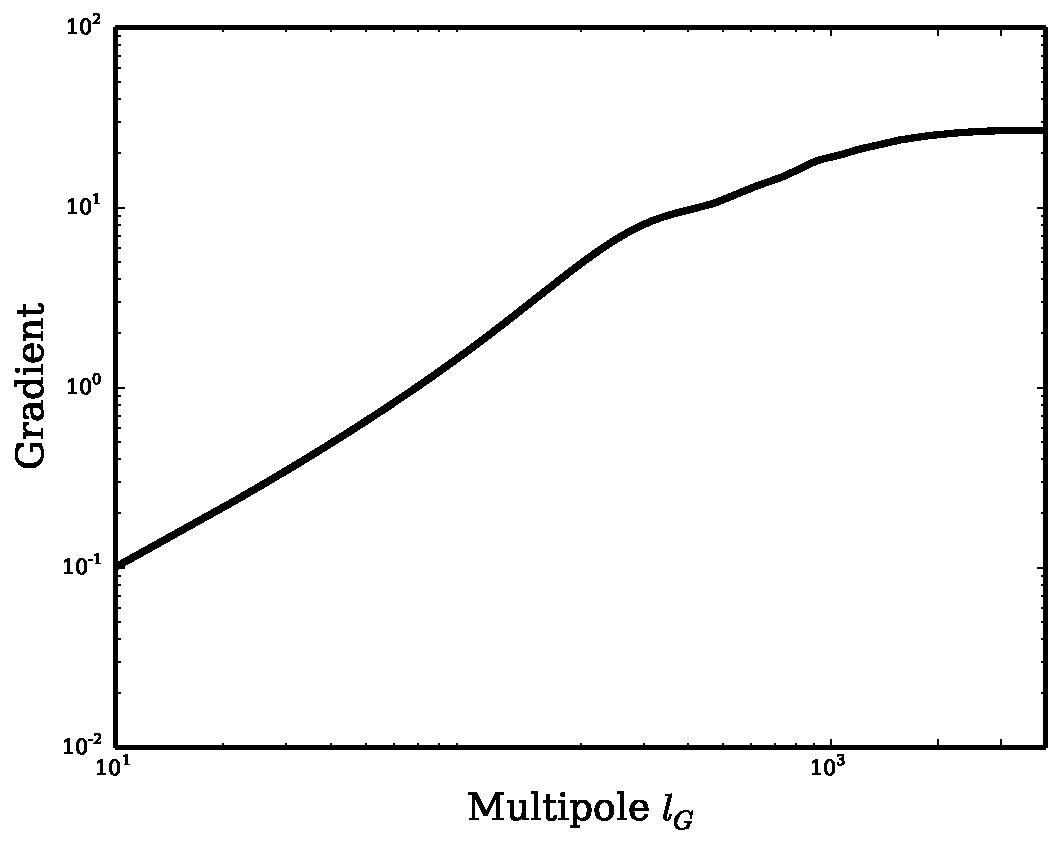
\includegraphics[width=\linewidth]{figs/gradient_cut.pdf}
\caption{Gradient of temperature field as a function of low pass filter l = $l_{G}$. It is dominated by mulitpoles below 2000. \pending{check the magnitude of Grms}}
\label{fig:gradient_cut}
\end{figure}

 
\section{modifications of Quadratic Estimator}
The major foreground in CMB cluster lensing analysis is thermal Sunyaey -Zel'dovich (tSZ) effect. 
tSZ effect is an order of magnitude greater than lensing signal; if not taken into consideration it induces systematic bias and varianace in the final convergence maps.
In this section we describe the modifications of Quadratic Estimator to make it robust to both tSZ induced bias and variance.

\subsection{modified Quadratic Estimator}
While designed to pull the lensing induced correlations, QE is equally sensitive to any other signal present in both G and L maps.
%The major systematic for lensing analysis is thermal Sunyaey -Zel'dovich (tSZ) effect, which is an order of magnitude greater than lensing signal biases the analysis if not taken into account. 
 tSZ present in both maps results in a low bias.
 One way to eliminate tSZ bias is using tSZ free maps, which are constructed by exploiting the frequency dependance of tSZ signal.
 %Previous studies either used a tSZ free map or a more stringent low pass filtering of the gradient map.
 %tSZ is frequency dependent signal and hence we can use multiple frequency channels to eliminate tSZ. 
 However, this results in a increased statistical uncertainty in the reconstructed convergence profile.
 Another way to mitigate the bias is by using a more stringent low pass filter on the gradient map. %; by having a more robust seperation of scales between gradient map and small scale map.
 By having a more robust seperation of scales between gradient map and small scale map.
 While this can reduce the bias significantly, this results in a poor gradient estimation and hence increasing the statistically uncertainty.

 
 During my thesis we came up with a novel approach to completely remove the tSZ bias. 
 Any foreground signal which is present in both the maps will lead to a systematic bias, so by getting rid of the foreground signal in one of the maps (either G or L) should eliminate the bias completely.
  As shown in Fig.~\ref{fig:gradient_cut}, most of the gradient estimation comes from multipoles l <2000 and CMB is not limited by noise at those scales.
  So, natural choice would be to eliminate tSZ in the gradient map by using linear combination of different frequencies. 
  In modified Quadratic Estimator, eqn 3.6 becomes,
  \begin{equation}
   G(\hat{n}) = \nabla (\int\frac{d^{2}l}{(2\pi)^{2}} e^{il .\hat{n}} W^{TT}_{l} T^{SZ_free}_{l}   )
  \end{equation}
  where $T^{SZ_free}_{l} $ is the tSZ-free map.
\section{Data}
\label{sec_data}
We use data sets from two different experiments: CMB maps from South Pole Telescope is explained in \S\ref{sec_SPT} and 
optical cluster catalog from Dark Energy Survey is explained in \S\ref{sec_DES}

\section{South Pole Telescope}
\label{sec_SPT}
South Pole Telescope (SPT) is a 10 meter diameter, wide field, offset Gregorian telescope \citep[SPT,][]{padin08, carlstrom11} located at the Amundsen-Scott South Pole station.
The SPT has been operating since early 2007 and has completed two surveys so far: SPT-SZ (2007 -2011) and SPTpol (2012-2016).  
Extremely dry and stable atmosphere of the south pole makes it one of the best available sites on Earth for observing millimeter and sub-millimeter wavelengths. 

\subsection{\sptpol{} {\rm 500} deg$^{2}$ survey}\label{sec_sptpol}
\sptpol{} is the second camera installed on the \mbox{10-meter} South Pole Telescope \citep[SPT,][]{padin08, carlstrom11} located at the Amundsen-Scott South Pole station.
The \sptpol{} focal plane consists of 1536 polarization-sensitive transition edge sensor bolometers (360 at 95 GHz and 1176 at 150 GHz) \citep{austermann12}.
%enabling polarization observations \citep{austermann12}.
The \sptpol{} 500~deg$^{2}$ survey spans fifteen degrees of declination, from -65 to -50 degrees, and four hours of right ascension, from 22h to 2h. 
%In this work we use the temperature (T) and polarization (Stokes Q and U) maps of the CMB from observations between April 2013 to September 2016 in the frequency bands 95 GHz and 150 GHz. 
In this work, we use CMB temperature maps from observations between April 2013 and September 2016 in frequency bands centered at approximately 95 GHz and 150 GHz. 
The telescope beam and pointing solutions were characterized using Venus and bright point sources in the \sptpol{} survey region. 
The final telescope beam along with the pointing jitter roughly corresponds to a $\theta_{\rm FWHM} = 1.^{\prime}22\ (1.^{\prime}7)$ Gaussian for the 150 (95) GHz dataset.

We briefly summarize the procedure we use to reduce raw CMB data to maps and refer the reader to \cite{henning18} for further details. 
The raw data are composed of digitized time-ordered data (TOD) for each detector that are converted into CMB temperature units. %% using a Planck-based calibration factor. 
We bin the TOD into two different maps using a flat-sky approximation in the Sanson-Flamsteed projection \citep{calabretta02, schaffer11}. 
To construct the first map, in which we aim to reconstruct the small-scale lensing signal, we remove large-scale modes $\ell \le 300$, bandpass filter the TOD in the range of approximately $300 \le \ell_{x} \le 20,000$, and bin them into 0.\am5\ square pixels.
For the second map, intended for estimation of the large-scale CMB gradient, we apply minimal TOD filtering by only removing modes below $\ell_{x} \le 30$, and bin them into 3\am\ square pixels.
While we only use the data from the 150 GHz channel for the first map, the latter is a tSZ signal cleaned map produced by linearly combining the 95 and 150 GHz channels. 
We use this tSZ-free map to reconstruct the background gradient of the CMB at the cluster locations.
As we will see later in \S\ref{sec_method_QE}, the gradient estimation using the tSZ-free map helps in removing the tSZ-induced lensing bias.
The minimal filtering on this map allows us to recover large-scale modes which indeed helps in a better estimation of the background gradient.
The 0.\am5{} resolution 150 GHz map has a white noise level of \mbox{$\Delta_{\rm T} = $ 6 \ukam} estimated using a jackknife approach. %estimated within the multipole band $4500 \le \ell \le 7500$.
The low-resolution tSZ-free combination is noisier with \mbox{$\Delta_{\rm T} \sim $ 17 \ukam}.
\pending{Noise power spectrum plot}
%%%\pending{Pending: SR: Should we quote this? Can we trust this number?}
%\section*{Cosmic Microwave Background cluster lensing}
\subsection{DES and the {\rm \RM} catalog}\label{sec_DES}
The Dark Energy Survey (DES) was a $\sim$5000 \sqdeg, optical to near-infrared survey conducted using the Dark Energy Camera \citep{flaugher15} mounted on the 4-meter Victor Blanco telescope at Cerro Tololo Observatory in Chile and has recently finished its survey. 
For this analysis, we use the cluster catalog obtained from the first three years of DES observations, which almost covers the \sptpol{} 500\,deg$^{2}$ survey. 

%The cluster catalog was derived using the RM algorithm \citep{rykoff14}  from the DES photometric datasets. 
The cluster catalog was derived using the RM algorithm \citep{rykoff14}.
RM is an optical cluster-finding algorithm which detects candidates by identifying over-densities of luminous red galaxies with luminosity greater than 20\% of $L_{*}.$
%Milky Way ($0.2L_{*}$). [I DON'T THINK THIS IS ACTUALLY THE DEFINITION OF L* (TC\citetalias{mcclintock18})]
It is based on our understanding that galaxy clusters are agglomerations of galaxies containing old and subsequently red stars. 
The algorithm iteratively assigns membership and centering probabilities for each red galaxy identified as belonging to a cluster candidate. 
A weighted sum of the membership probabilities, richness $\lambda$, is assigned to each candidate.
The centre comes from the galaxy with the highest centering probability.
The DES RM catalog contains two samples: a flux-limited sample and a volume-limited sample. 
The flux-limited sample has more high-redshift clusters detected from deep fields in the survey. 
On the other hand, the volume-limited sample is independent of survey depth, complete above a luminosity threshold \citep[hereafter \citetalias{mcclintock18}]{mcclintock18}, and normally preferred for cosmological analysis.
% (hereafter referred to as the volume-limited sample).
See \citet{rykoff16} for more information on the application of RM to the DES survey data.

The RM cluster catalog version employed in this analysis is \whichcatversion. 
The \whichyear{} gold catalogue is based on the previous catalog from the Year-1 data \citep{drlica-wagner17} with some updates described in \citet{morganson18}.
The catalog contains 54,112 clusters above richness $\lambda \ge 20$ in the flux-limited sample and 21,094 clusters in the volume-limited sample. % \pending{(Pending: Cite DES Y3 cat. paper)}. 
Of these, 5,828 (2,428) clusters from the flux(volume)-limited sample lie within the \sptpol{} 500 \sqdeg{} survey  in the redshift range $0.1 \le z \le$ 0.95 (0.90). 
%We additionally remove clusters near the survey edges or within $10^{\prime}$ distance from a bright ($\ge 50$ mJy at 150\,GHz) point source.
We additionally remove clusters near the survey edges by removing the cutouts (see \ref{sec_cluster_cutouts}) with more than 5\% masked pixels or within $10^{\prime}$ distance from any bright ($\ge 6$ mJy at 150\,GHz) point sources detected in the \sptpol{} temperature map.
%we use data/500sqdeg_bleem/quick_mm_point_source_file_150.0GHz_6.00000mJy.txt.
These cuts leave 4,003 (1,741) clusters with $\lambda \ge 20$ from the flux(volume)-limited sample with a median redshift of $\tilde{z}$ = 0.77 (0.48). 
The error in the cluster photo-$z$ estimates are small with $\hat{\sigma}_{z} = 0.01 (1+z)$ \citep{rozo15}.
\pending{include a figure with SPTpol map and pointing to a cluster}
%\pending{Finally, we impose a cut on the cluster richness and remove all clusters above $\lambda \ge 60$ that removes \pending{xx (xx)} from the full (cosmology) sample. This cut was motivated based on the results from Sehgal sims described in \S\ref{sec_xx_xx}}.
%Cosmic Microwave Background (CMB) photons while passiang through intervening galaxy cluster gets lensed and we call this phenomenon as CMB-cluster lensing.
% Lensing remaps the unlensed CMB field based on the angular deflection caused by cluster gravitational potential.
 %In mathematical form CMB cluster lensing can be written as the equation below
 %\begin{eqnarray}
%T(\hat{\textbf{n}})& = & \widetilde{T} (\hat{\textbf{n}} + \vec{\alpha}(\hat{\textbf{n}}))\\
%Q(\hat{\textbf{n}}) & = & \widetilde{Q} (\hat{\textbf{n}} + \vec{\alpha}(\hat{\textbf{n}}))\\
%U(\hat{\textbf{n}}) & = & \widetilde{U} (\hat{\textbf{n}} + \vec{\alpha}(\hat{\textbf{n}}))
%\end{eqnarray}
%where $ \widetilde{T}$ is unlensed temperature field, $\widetilde{U}$ and $\widetilde{Q}$ are the unlensed polarisation fields.
%$\vec{\alpha}(\hat{\textbf{n}})$ denotes the deflection angle and is directly proportional to the mass of the galaxy cluster.

%Lensing signal by an individual cluster is too weak to detect, so we need to stack many clusters to obtain a significant signal.
 %For example, the lensing induced distortion due to a $2 \times 10^{14} \ M_{\odot}$ mass galaxy cluster  is $\sim 5.0$ and $0.5 \ \mu K$ in temperature and polarization respectively.
%In this chapter, we will discuss various methods available in literature to extract CMB-cluster lensing signal. 
%The chapter is organized as follows 
 \subsection{fitting model}
To obtain the mass of the cluster, we need to compare the observed lensing profile to the convergence model generated using an assumed halo mass profile.
 The observed lensing convergence profile of cluster has contributions from its own halo density ($k_{1h}$) as well as from the correlated structures along the line of sight known as two halo term ($k_{2h}$).
 For $k_{1h}$, we assume the galaxy cluster density to follow Navarro Frenk White (NFW) profile and in \ref{sec_systematics} we quantify the robustness of this assumption by using Einasto profile \citep{Einasto}
 A NFW halo profile is characterized by its scale radius $R_{s}$, the dimensionless concentration parameter c, and the dimensionless charateristic over-density $\delta_{c}$.
 The characteristic over density is defined as the ratio central cluster density to the critical density of the Universe at the cluster redshift.
 In terms of these quantities the NFW halo density profile is written as 
 \begin{equation}
 \rho(r) = \frac{\delta_{c}\rho_{crit,z}}{(\frac{r}{R_{s}})(1 + \frac{r}{R_{s}})^{2}}
 \end{equation} 
 where $\rho_{crit,z}$ is the critical density of the Universe at cluster redshift.
 
 The lensing convergence profile is the ratio of surface mass density to the critical surface density of the Universe at cluster redshift, $k(x) = \frac{\Sigma(x)}{\Sigma_{crit}}$, where
 \begin{eqnarray}
 \Sigma(x) = 2 \int^{\inf}_{0} \rho(r) ds\\
 \Sigma(crit) = \frac{c^{2}}{4\pi G} \frac{D_{CMB}}{D_{clus} D_{CMB,clus}} 
 \end{eqnarray} 
Here r is the distance from the center, x is the corresponding projection on the plane,$D_{CMB}$ and $D_{clus}$ are the comoving distances to the CMB and galaxy cluster respectively; $D_{CMB,clus}$ is the distance between the CMB and the cluster.

We model the two halo term, $k_{2h}$, by using the Eq. 13 of \pending{Oguri and Hamana}.
With model prediction in hand we can write down the likelihood of observing the data as:
\begin{equation}
-2 ln L (k | M) = (k - k_{m})(M) C^{-1} [(k - k_{m})]^{T}
\end{equation}
where $k$ is the observed lensing convergence profile, $k_{m}$ is lensing convergence for NFW profile at mass M, and C is the covariance matrix. 
Note that the contribution from the two halo term is considered only for real and not the pipeline verification in \S\ref{}

\section{cluster cutouts and weighing scheme}

We extract 300\arcmin square box form SPTpol temperature maps at the DES cluster locations. 
While the boxsize is much larger than the virial radius of the cluster, it is necessary to robustly approximate the background gradient. 
This is because much of the gradient power comes from larger scale modes, reducing the analysis to a smaller box will reduce the SNR of the mass estimation. 
These cutouts are then passed through the pipeline to extract lensing convergence profile. 
After extracting the convergence profile, we limit modelling and likelihood calculations to 10\arcmin box around a cluster.

As mentioned before, the lensing signal is weak for individual cluster and we need to stack lensing convergence profiles to increase the SNR of detection.
While

 
%\section{NFW profile}
The schematic representation of Quadratic Estimator is shown in Fig 2. 
Panel (a) is the 10\arcmin X 10\arcmin cutout of the observed temperature map, $T_{l}$.
This is filtered in the fourier space \pending{mention equations} to obtain the filtered gradient and lensing maps, shown in panel (b) and (c) respectively.
Lensing convergence profile (panel (c)) is reconstructed by extracting the correlations between lensing and gradient maps.
 \begin{figure}[H]
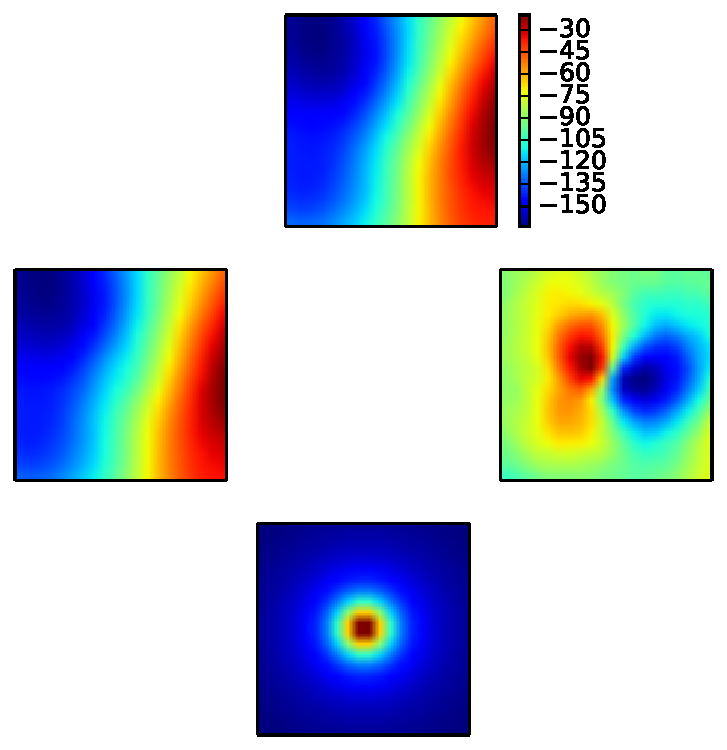
\includegraphics[width=\linewidth]{figs/schematic_rep.pdf}
\caption{Gradient of temperature field as a function of low pass filter l = $l_{G}$. It is dominated by mulitpoles below 2000. \pending{check the magnitude of Grms}}
\label{fig:gradient_cut}
\end{figure}
  \section{Results and Discussion}\label{sec_results}

The main results of this work are the lensing-derived cluster mass constraints for the DES RM \whichyear\ cluster samples using \sptpol{} tSZ-free $\times$ 150 GHz temperature maps.
%using three different combination of the \sptpol{} and \planck{} temperature maps: (A) \sptpol{} tSZ-free $\times$ 150 GHz maps (baseline); (B) \lgmca $\times$ \sptpol 150 GHz maps; and (C) baseline $+$ \sptpol{} tSZ-free $\times$ tSZ-free maps for clusters with $\lambda \ga 40$.
Below, we first present the lensing mass estimates in \S\ref{sec_temp_results} and use the lensing measurements from the DES \whichyear{} volume-limited sample to independently calibrate the \ML{} relation of the cluster sample in %\S\ref{sec_ML_scaling}. 
\subsection{Stacked mass measurements}
\label{sec_temp_results}
In Fig. \ref{fig_QE_stacked_maps}, we present the results of our stacked lensing measurements. 
The left (right) panel correspond to the convergence maps stacked at the location of clusters in the DES \whichyear\ flux(volume)-limited sample.
The variance in the flux-limited sample is lower than the volume-limited sample because the flux-limited sample has twice as many objects. 
An estimate of the mean-field has been subtracted from the maps.
We reject the null hypothesis of no lensing with a significance of \howmanysigmaforfullsample\ for the flux-limited sample of \howmanyclustersinfullsample\ clusters. 
The obtained \snr{} is consistent with our expectations from the simulations shown as lighter black circles in %Fig. \ref{fig_QE_sehgal_sims}.
For the smaller volume-limited sample, the no-lensing hypothesis is ruled out at  \howmanysigmaforcosmosample.
The radially binned convergence profiles that are used to estimate the cluster masses are shown in Fig. \ref{fig_QE_stacked_maps_radprf} along with the best-fit model curves. 
\begin{figure}
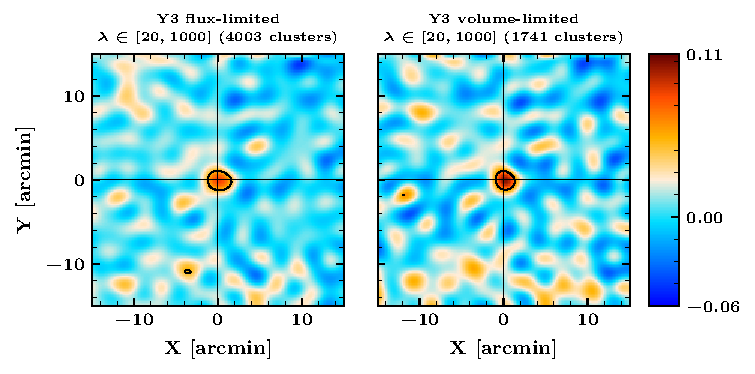
\includegraphics[width=\linewidth]{figs/kappa_model_MF_y3_v6_4_22_full_vl_JODY.pdf}
\caption{It shows}
\label{fig:fig_QE_stacked_maps}
\end{figure}

\begin{figure}
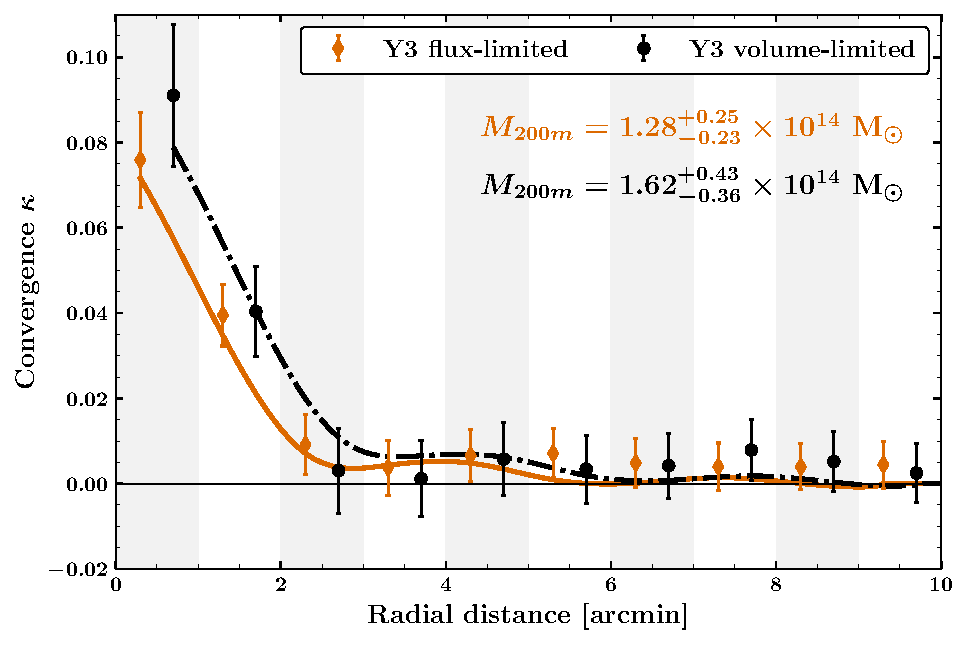
\includegraphics[width=\linewidth]{figs/kappa_model_MF_y3_v6_4_22_full_vl_radprf_JODY.pdf}
\caption{It shows}
\label{fig:fig_QE_stacked_maps}
\end{figure}

The ringing pattern is because of the sharp filtering of modes above the \sptpol{} beam scale. 
The error bars plotted are the square root of the diagonal entries of the covariance matrix estimated using %Eq. (\ref{eq_JK_cov}). 
%As explained in \S\ref{sec_nfw_model_fitting}, all the mass estimates are derived by fitting a NFW profile along with the contribution from the {\it 2-halo} term to the measured radially binned profile. 
The recovered lensing masses for the stacked flux and volume-limited samples are %\mbox{\mvir = \fitmassforfullsamplewitherrors\ \times \munits} and \mbox{\fitmassforvlsamplewitherrors\ \times \munits} respectively. 
According to expectations, the lensing masses shift up by 0.3$\sigma$ when the {\it 2-halo} term is excluded.


A higher mean mass is expected for the volume-limited sample. 
At redshifts above $z\sim 0.6$, galaxies at the luminosity threshold adopted by RM become too faint to be detected in the DES data. 
Consequently, the richness of the clusters is extrapolated from the subset of galaxies that are sufficiently bright to be detected. 
This extrapolation introduces additional noise in the richness estimates.
The increased scatter leads to more low-mass systems scattering up to apparently rich systems, thereby lowering the mean mass of the selected halos. 
For this reason, we restrict our analysis to the volume-limited sample in the subsequent sections. 
\subsection{Mass-richness \ML{} scaling relation calibration}\label{sec_ML_scaling}

We now apply the lensing mass measurements from \S\ref{sec_temp_results} to constrain the relationship between a cluster's mass, $M$, and optical richness, $\lambda$, in the DES RM \whichyear{} volume-limited sample. 
We limit the analysis to just the volume-limited sample since the flux-limited sample has selection bias as explained above in \S\ref{sec_temp_results}.
%Due to its higher S/N, we use the QE  with a tSZ-free gradient map; we do not combine the two estimators due to the complexity in combining the different bases of the MLE and QE. 
Following earlier weak-lensing analyses of RM clusters \citep{simet18, melchoir17, mcclintock18}, we use a power-law scaling relation for cluster mass, $M$, as a function of richness, $\lambda$, and redshift, $z$,
\begin{eqnarray}
M = A \left(\frac{\lambda}{40}\right)^{\alpha} \left(\frac{1+z}{1+0.35}\right)^{\beta},
\label{eq_ML}
 \end{eqnarray}
 where $A$ is a normalization parameter, and the exponents $\alpha$ and $\beta$ are richness and redshift evolution parameters respectively. 
The pivot points for the richness and redshift evolution were set based on DES weak-lensing measurements of \citetalias{mcclintock18}.
%Given the total\snr{}is of order eight for the flux-limited sample, we do not subdivide the stacks into different richness or redshift bins. 
The model for the stacked mass is 
\begin{equation}
M(A, \alpha, \beta) \equiv M = \frac{\sum_j w_j M(\lambda_{j}, z_{j})}{\sum_j w_j}, 
\label{eq_model_ML}
\end{equation}
where the sum runs over the number of clusters in the sample and the weight $w$ for each cluster is given in Eq. (\ref{eq_cluster_weight}).

We do not split the stacks into different richness or redshift bins.
As a result, the data's sensitivity to the two evolution parameters is minimal and we apply informative priors to both.
We perform a Markov chain Monte Carlo (MCMC) analysis %with 100 walkers and 750 steps each 
using the publicly available \emph{emcee} \citep{mackey13} code to sample the likelihood space.
%The first 100 steps from all walkers were discarded as the burn-in phase.
\begin{figure}
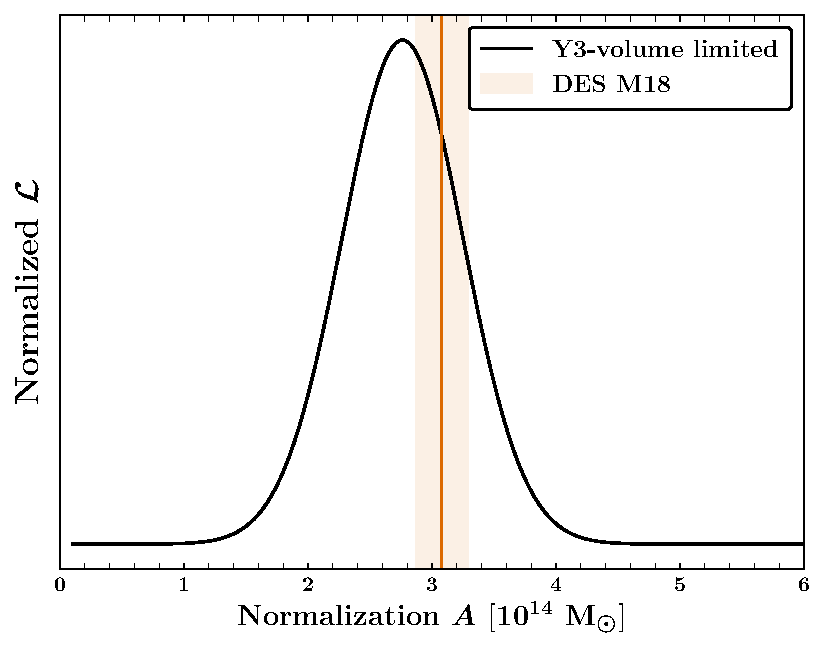
\includegraphics[width=\linewidth]{figs/M_rich_fitting_y3_v6_4_22_full_vl_JODY.pdf}
\caption{It shows}
\end{figure}


%  -------  Template Fitting  -------  
\setcounter{chapter}{3} %4
		 \chapter{Template Fitting}
\label{ch:template}

The modified Quadratic Estimator (mQE) developed in the last chapter completely eliminates the thermal Sunyaev-Zel'dovich (SZ) bias by using a SZ free gradient map. 
Though SZ bias is removed in the mQE, SZ present in the second leg induces extra variance in the reconstructed lensing convergence profile. 
Unlike the variance due to other sources (such as instrumental noise, uncorrelated foregrounds etc.,), SZ variance depends on the mass of the galaxy cluster.
The SZ variance scales roughly with the mass of cluster as $M^{5/3}$.
For DES X SPTpol clusters which we used in the last chapter, we downweighed the massive clusters to take the SZ variance into account. 
This didn't have much effect on the final SNR as we had only few massive clusters. 
However, with future low noise CMB surveys such as SPT-3G, CMB-S4, Simons Observatory etc., downweighing won't be an optimal solution.
This chapter is organised as follows: in  \S\ref{sec_methods} we describe the template fitting approach which will significantly reduce the SZ variance, followed by results in \S\ref{temp_fit_sec_results}. 
We forecast mass uncertainties for future experiments using our new method in ~\S\ref{forecasts} and then we finally conclude in \S\ref{temp_fit_conclusions}.

%I present template fitting approach which will significantly reduce the SZ variance in high mass cluster and/or low noise surveys. 
%I then discuss the effect of SZ variance and experimental variance as a function of experimental noise and cluster mass. 
\section{Simulations}
\label{sec_simulations}

We use simulations to validate our new method and also to forecast future experiments. 
The simulations in this chapter are generated similarly to chapter \ref{ch:MLE}.
Briefly, we create \mbox{$100^\prime \times 100^\prime$} unlensed Gaussian realizations of the \textit{Planck} 2015 \citep{planck15-13} best-fit lensed CMB power spectrum obtained from CAMB\footnote{\url{https://camb.info/}} \citep{lewis00}.
These maps are then lensed by the cluster's convergence profile (see \S\ref{sec_def_field}). 
We add simulated SZ emission (\S\ref{sec_tsz}) and then convolve the map
 by the assumed instrumental beam. 
We take the instrumental beam to be Gaussian with a FWHM $=1^\prime.7$ at 90 GHz and $=1^\prime.0$ at 150 GHz. 
Finally, we add Gaussian realizations of white noise at the specified noise level. 
 


\subsection{thermal Sunyaev-Zel'dovich signal}
\label{sec_tsz}

Unless otherwise noted, we assume the SZ emission is described by a radially-symmetric  Arnaud profile \citep{arnaud10} expected for a cluster of the specified mass and redshift. 
We do test the robustness of this assumption in \S\ref{subsec:simsz} by using two sets of realistic SZ simulations from \citet{sehgal10} and \citet{takahashi17}. 
The SZ power in the \citep{sehgal10} simulations is scaled down by a factor of 1.75 to better match the measured SZ power in \cite{george15}; the \citet{takahashi17} simulations post-date the SZ measurements and are not rescaled. 
Extracting the appropriate SZ signal from these simulations requires selecting matching galaxy clusters, with a tradeoff between the number of matching clusters in the simulations and the fidelity of the match. 
 We randomly select halos which are within 5\% of the desired mass and $\pm 0.2$ of the desired redshift.

\section{Method}
\label{sec_methods}
In this section, we present a template fitting approach designed to reduce the SZ variance for massive galaxy clusters or for low noise surveys. 
We also discuss sources of uncertainties present in the CMB-cluster lensing analysis. 
\subsection{Template fitting to reduce the SZ variance}
\label{sec_sz_template_fitting}

An obvious way to eliminate the SZ variance is by using SZ-free maps for both the small-scale and gradient maps. 
Of course this would undo the advantages of the modified QE for the instrumental noise in the small scale map. 
One can also reduce this extra variance by projecting out a model template for the SZ signal, and thereby reducing the total amount of SZ power in the small-scale map. 
Given the impossibility in creating a `perfect' SZ template, the template fitting will not completely eliminate the SZ signal in the small-scale map. 
However, template fitting can significantly reduce the SZ power in the small-scale map, and thus reduce the SZ noise penalty on the lensing mass reconstruction. 



To be unbiased, we must fit the template to a CMB-subtracted map or account for the information loss from template projection in the normalization factor $A_l$ of Eqn.~\ref{mqe_convergence_eqn}. 
The latter tact (correcting $A_l$) might have advantages if one needed to suppress multiple kinds of cluster emission, e.g., dusty and radio galaxies in addition to the thermal SZ effect. 
Projecting a template from the Compton-$y$ map will not help these other cluster signals. 
However, we expect these other signals to be small compared to the SZ flux for massive galaxy clusters. %\pending{citations needed}. 
In this work, we take the first approach and fit the template to a Compton-$y$ map created from a linear combination of 95 and 150\,GHz maps. 
Effectively, we have used the different spectral dependence of the SZ and CMB to eliminate the CMB, and thus any correlation between the removed template and the lensing dipole in the CMB map. 

\begin{figure}[ht]
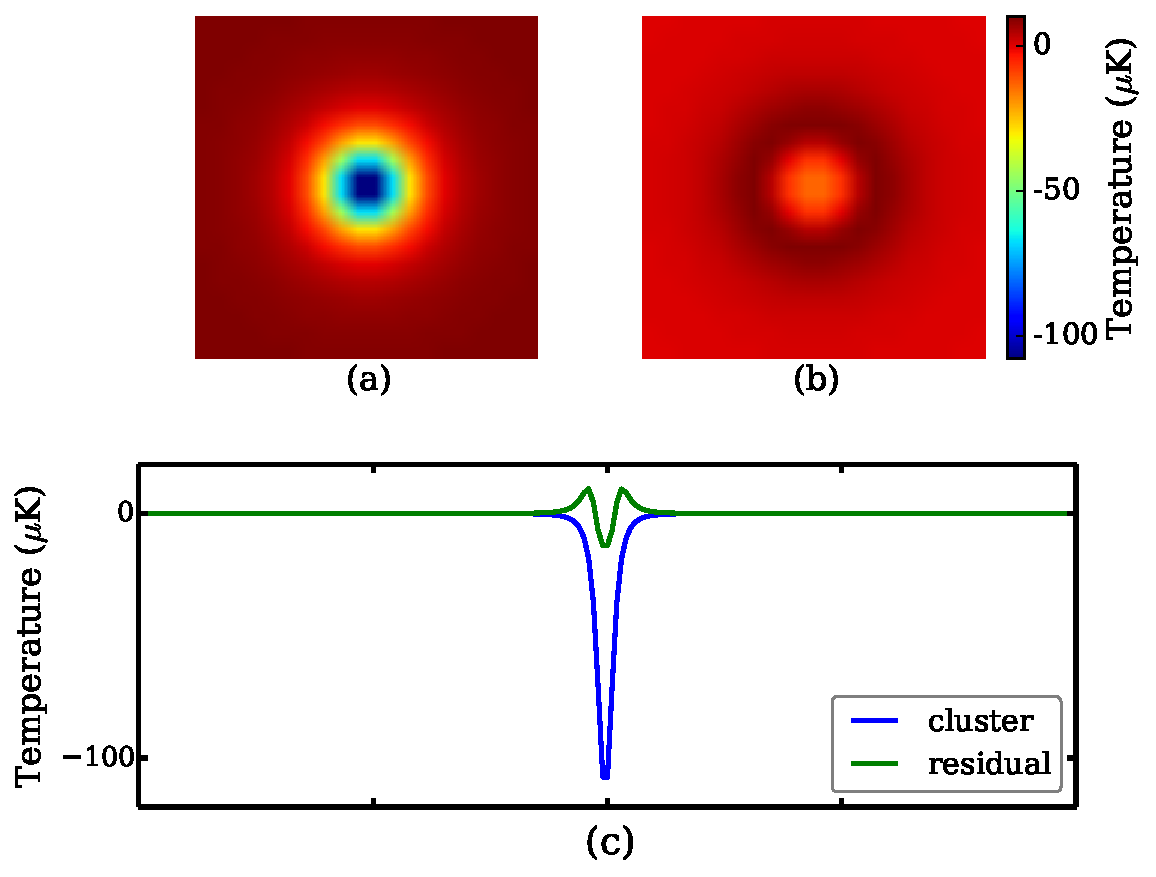
\includegraphics[width=\linewidth, keepaspectratio]{figs/template_fitting.pdf}
 \caption{Template fitting significantly reduces SZ power, even with an imperfect match between the template and true SZ signal. 
The top left panel (a) shows the expected Arnaud profile for a galaxy cluster of mass $\mvir = 5 \munits$ at z=0.7 after being smoothed by Gaussian beam with FWHM= 1\arcmin.7.
The top right panel (b) shows the residuals after subtracting the best-fit 2\arcmin.0 FWHM Gaussian (the amplitude is free, but the FWHM is fixed). 
The lower panel (c) shows one-dimensional slices through each panel: the solid, blue line is a slice through the beam-convolved Arnaud profile of (a), and the dashed green line is a slice through the residual map in (b). 
 } 
\label{fig:residual}
\end{figure}
We choose to use a radially symmetric template at the fixed cluster location in this work. 
Unless otherwise noted, we assume the beam to be a Gaussian with FWHM = 1\arcmin{} at 150\, GHz and 1\arcmin.7 at 90\,GHz. 
As this beam size is significantly large compared to the actual size of clusters at $z>0.3$, clusters are approaching the effective point source limit where the specific details of their shape would not matter. 
Thus we choose to use a simple Gaussian template as the baseline template in this work. 
We also compare the results to template fitting with more physically motivated Arnaud profile \citep{arnaud10}, convolved by the experimental Gaussian beam.  
The residuals of removing a 2\arcmin.0 FWHM Gaussian from an Arnaud profile convolved by a 1\arcmin.7 beam are illustrated in Fig.~\ref{fig:residual}. 
As argued above, the Gaussian template significantly reduces the SZ signal despite the mismatch between the assumed profile and input SZ model. 
While there should be small variations in the typical size of the cluster's SZ emission with mass and redshift, we neglect these variations and fix the size of the templates based on the expected median mass and redshift of the sample. 
One could easily adjust the template based on individual cluster redshift for a minimal increase in complexity.



As SZ and CMB have different frequency dependence, we use linear combination of 95\, GHz and 150\, GHz channels to obtain Compton-$y$ maps.
%\begin{equation}
%T_{sz} = \frac{B_{90}}{B_{150}} T_{90} - T_{150} 
%\end{equation}
%Since the template will be applied to that small-scale map that has been high pass filtered at $\ell > 2000$, we apply a matching high pass filter to the map used for fitting and the SZ model template. 
We then pull out a central $10\arcmin \times 10\arcmin$ cutout at the cluster location for fitting the template. 
Since both the SZ emission and lensing signal extraction is concentrated within a few arcminutes of the cluster center, there is little reason to fit over a larger area. 
We allow for two free parameters in the fitting: the overall amplitude of the template, and a constant DC background level. 
%Note that given the high-pass filter, we expect (and find) the DC term to be effectively zero. 
We include the DC term while fitting the template amplitude, however, we do not subtract DC level. 
Only the template is subtracted from the small-scale lensing map.



With template fitting included, the Fourier transforms of the two maps used by the quadratic estimator can be written down as:
\begin{eqnarray}
G_{\ell} &=& i\ell W^{G}_{\ell} T^{\rm SZ-free}_{\ell}\\
L_{\ell} &=& W^{L}_{\ell} \left(T_{\ell} - T_\ell^{\rm SZ-template}\right)
\end{eqnarray}
where, $G_{\ell}$ is the large-scale gradient map and $L_{\ell}$ is the small-scale map. 
$W^{G}_{l}$ and $W^{L}_{l} $ are the Wiener filters to maximize the lensing signal \cite{hu07}. 
The mm-wave map is $T_{\ell}$ while the constructed SZ-free map is $T^{\rm SZ-free}_{\ell}$. 
Compared to the modified QE \citep{madhavacheril18,raghunathan18}, the new element is the $T_\ell^{\rm SZ-template}$ term representing the SZ template fit. 





\subsection{Sources of uncertainty in the CMB-Cluster Lensing Measurement}
\begin{figure}[htb]
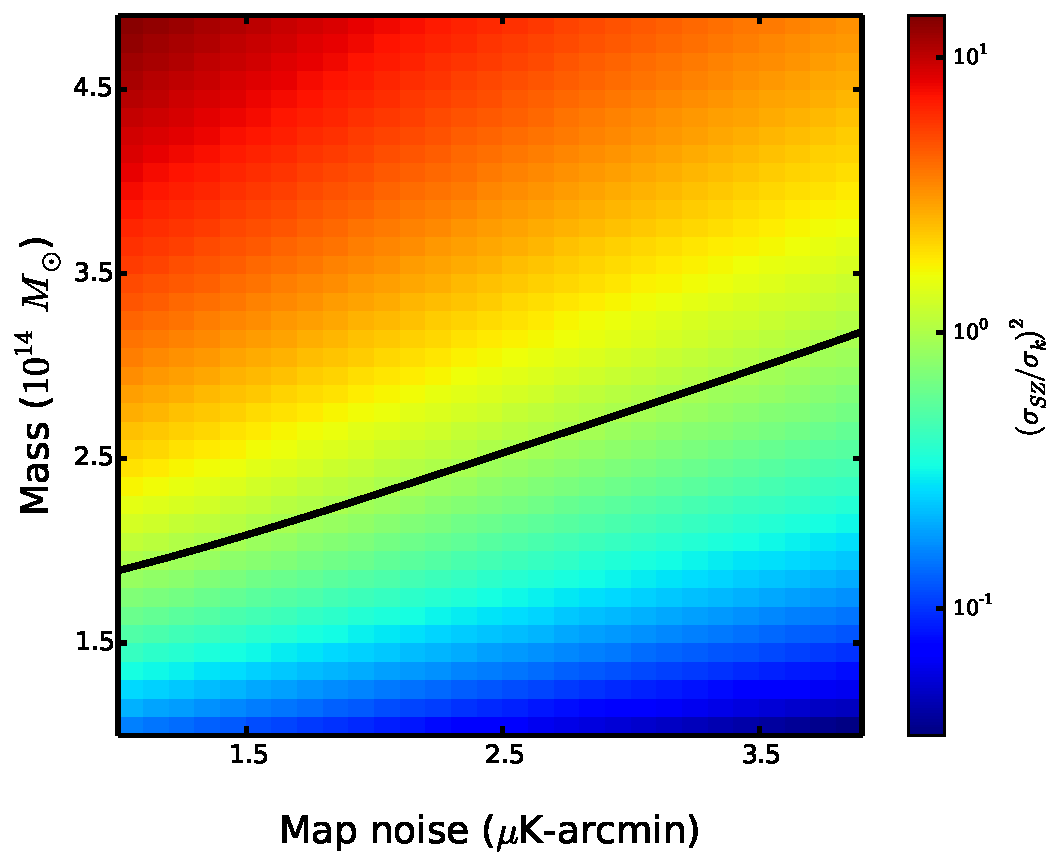
\includegraphics[width=\linewidth, keepaspectratio]{figs/contour_plot.pdf}
 \caption{
 Ratio of SZ variance over kappa variance as a function of cluster mass and experimental noise level. 
 As expected the ratio increases with mass for a given experimental noise level. 
 The black solid line represents the points where the ratio SZ variance is equal to that of experimental noise.
 %\pending{(SR 20190130: Can you make a contour plot here to also include the effect of map depth? That will be more intuitive and one can easily figure out the mass threshold for which this method will be effective for different surveys.)\\}
 %\pending{Axis labels and caption disagree: sigma/variance} 
 %\pending{\textbf{Plot change: Keep the dashed line for 'SZ variance'. Add several horizontal lines at eg 1uk-arcmin, 3-uk-arcmin, 10uk-arcmin. Y-axis will no longer be the ratio}}
  }
 \label{fig:variance}
\end{figure}

Template fitting is intended to reduce the SZ variance, however it will do nothing for other sources of uncertainty such as instrumental noise, CMB sample variance and foreground emission (if not cleaned). 
Thus it will be useful to look at the relative magnitudes of these two terms, the SZ variance ($\sigma_{SZ}^{2}$) and the non-SZ variance ($\sigma_{\kappa}^{2}$), when interpreting the performance of template fitting in the next section. 


The non-SZ variance depends on the survey parameters (i.e.~instrumental noise, and the degree to which foregrounds are cleaned) but is independent of the cluster properties. 
We estimate the non-SZ variance, $\sigma_{\kappa}^{2}$, using simulations of the CMB plus instrumental noise. 
Given the goal, we do not include the cluster's SZ emission.  
We apply the lensing pipeline to the simulated skies to estimate the convergence maps. 
We fit the convergence map  to determine  a mass, and take the scatter in these inferred masses over 1000 simulations to be $\sigma_{\kappa}$. 


In contrast, the SZ variance should increase with cluster mass, $M$, roughly as $\sigma_{sz}^2 \propto M^{5/3}$, while being independent of the survey parameters. 
We estimate the SZ variance using the same suite of simulations, however now adding the cluster's SZ emission to the small-scale lensing map. 
We continue using an SZ-free map for other leg of the QE, the large-scale gradient map. 
As before, we estimate the convergence maps, fit for masses and take the scatter in these inferred masses to estimate $\sigma_{SZ}^{2}$ + $\sigma_{\kappa}^{2}$.

We present the ratio of the SZ to non-SZ variances, $\sigma_{SZ}^{2}$/$\sigma_{\kappa}^{2}$, as a function of survey noise level and cluster mass in Fig.~\ref{fig:variance}.  
As expected, the ratio increases with mass at any given noise level. 
The black solid curve represents a ratio of unity when the SZ variance equals the non-SZ variance. 
We expect template fitting to significantly improve the mass uncertainties only for clusters above the black curve. 

\section{Results}
\label{temp_fit_sec_results}
%\pending{(SR 20190130: Have you tested the method for a slightly realistic tSZ profile like Sehgal?)} 

%In this section, first we quantify various sources of uncertanities in the final convergence maps as function of experimental noise level and cluster mass. 
%Later, we compare the performance of our new method for various templates. 
%We  then use some realistic SZ simulations to check the robustness of our method.
%Finally, we discuss the effects of miscentering on our lensing analysis.%three algorithms to estimate cluster masses:  
%(1) using an SZ-free map in the gradient leg and no SZ in the HPF leg of quadratic estimator 
%(2) using an SZ-free map only for the gradient leg of the QE, i.e. the modified QE, 
%and (3) improved version of the modified QE presented in this work, with an SZ-free map used for the gradient leg of the QE and projecting an SZ template out of the  HPF leg. 
%We rate the performance of each method,  as a function of both cluster mass and experimental noise levels,  by the estimated uncertainty on the recovered cluster mass. 



 \begin{figure}[thb]
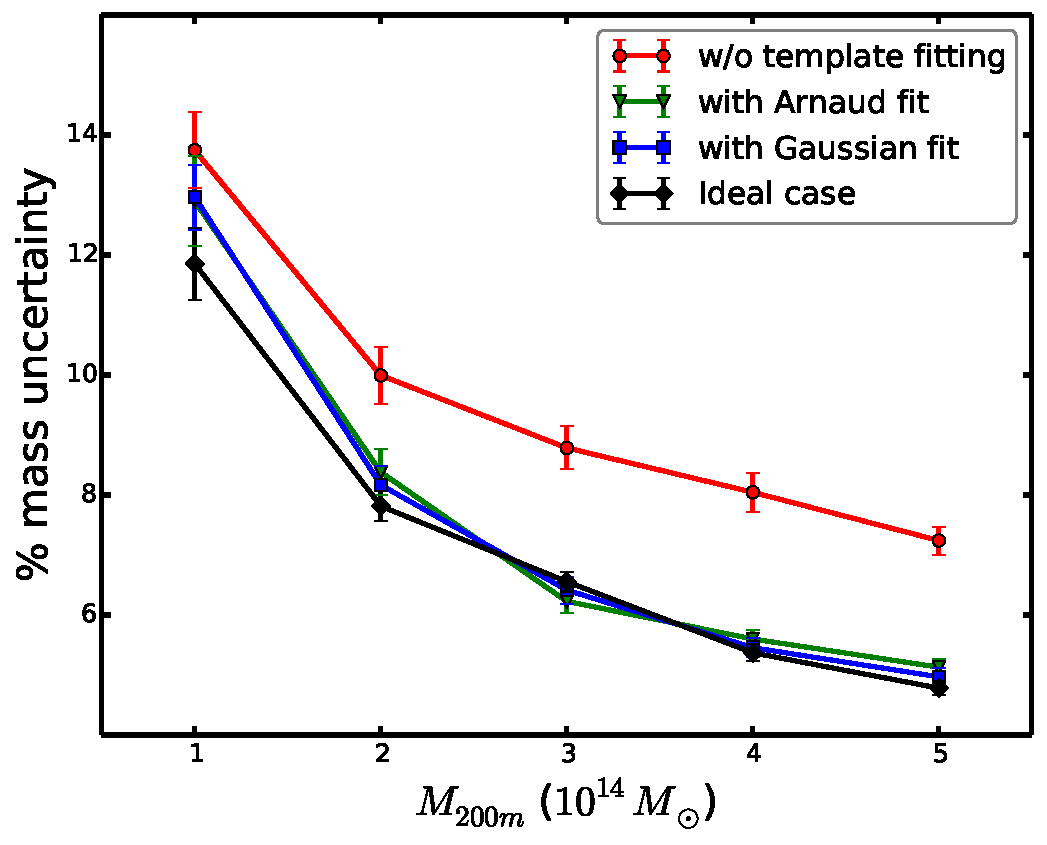
\includegraphics[width=\linewidth, keepaspectratio]{figs/uncen_vs_mass.pdf}
 \caption{
 Projecting out an SZ template from the second leg o the modified QE improves the performance for all masses considered. 
 Here we show the percentage mass uncertainties from three methods for a sample of 1000 clusters at a experimental noise level of 3\,\ukarcmin{}.
 All the curves use an SZ-free map for the gradient, but make different assumptions about the second, high-pass filtered map. 
\label{fig:template_fitting}}
\end{figure}

As shown in Fig.~\ref{fig:template_fitting}, we find that template fitting leads to a significant improvement in the final mass uncertainties for CMB-cluster lensing. 
For high-mass clusters, template fitting does nearly as well as in the idealized (non-physical) limit of having no SZ emission. 
In this figure, we are assuming an SPT-3G like experiment with FWHM of 1$^\prime$ and 1.7$^\prime$ at 150\,GHz and  95\,GHz respectively and a survey noise level of 3\,\ukarcmin{}. 
We compare four algorithms to estimate cluster masses. 
In all cases we use a SZ-free gradient map (from a linear combination of 95 and 150\,GHz maps). 
%The tSZ emission injected in the high-pass filtered 150\,GHz map is based on an Arnaud profile. 
First, the red solid line shows the performance of the original modified QE without template fitting, where we have used SZ-free gradient map and 150GHz map with Arnaud SZ for the high pass filtered map. 
%\sr{\sout{
%The second, black solid line shows the results for an idealized case, where we again use an SZ-free gradient map but use a 150\,GHz map without SZ for the small-scale map. 
%While the latter assumption is unphysical since there will be SZ emission at 150\,GHz, it is useful as a  representation of the performance limit for perfect SZ subtraction. }
The second, black solid line shows the results for an idealized case, where we use a 150\,GHz map without SZ for the high-pass filtered map. 
While this assumption is unphysical since there will be SZ emission at 150\,GHz, it is useful as a representation of the performance limit for perfect SZ subtraction. 
Note that the relative performance improvement between the idealized and baseline case increases with mass as expected. 
For these survey parameters, the idealized case has 17\% smaller uncertainties than the baseline for clusters of mass $1\times 10^{14}\,M_{\odot}$ and 50\% smaller for cluster masses of $5\times 10^{14}\,M_{\odot}$. 
Template fitting recovers nearly all of this gain for high-mass clusters, as shown by the green triangles and blue squares (we have introduced an offset along mass axis for clarity). 
The two lines reflect different templates for subtraction. 
%\sr{\sout{The input simulated SZ signal is based on an Arnaud profile in both cases.}}
The green triangle shows the performance of projecting out an Arnaud SZ template from the small-scale map. 
The blue square shows the results when using a Gaussian template instead, which is slightly mismatched to the assumed SZ signal. 
There is no practical performance difference between the two templates. 
For these assumed survey parameters, both templates are essentially indistinguishable from the idealized perfect SZ removal case at masses above $2\times 10^{14}\,M_{\odot}$. 
Template fitting does not do as well at lower masses. 
This can be understood by considering  the zero-mass limit -- where one tries to remove the SZ template from a map without SZ emission. 
The noisy estimate of the SZ template amplitude will set a non-zero, effective floor to the apparent SZ-like signal in this map. 
In the low-mass limit, SZ template removal will thus perform more poorly than the original estimator. 
The first signs of this transition can be seen in Fig.~\ref{fig:template_fitting} when comparing the performance at $\mvir = 2\times 10^{14}\,M_{\odot}$ to   $1\times 10^{14}\,M_{\odot}$.


 
 
%%%%%%%%%%%%%%%%%%%%%%%%%%%%%%%%%%%%%%%%%%%%%
%%%%%%%%%%%%%%%%%%%%%%%%%%%%%%%%%%%%%%%%%%%%%
%%%%%%%%%%%%%%%%%%%%%%%%%%%%%%%%%%%%%%%%%%%%%



%To calculate $\sigma_{\kappa}$, we use simulated tSZ free gradient and 150GHz maps, calculate the standard deviation within 10' from the center of the corresponding 'null' convergence maps. 
%The variance induced due to SZ is considerable for the clusters where ratio of $\sigma_{sz}/\sigma_{\kappa}$ is greater than 1. 
 
%\begin{figure}[h!]
%\includegraphics[width=\linewidth]{template_fitting_likelihood.png}
 %\caption{\pending{}}
 %\label{fig:boat1}
%\end{figure}
\iffalse{
\subsection{Miscentering}
\begin{figure}[ht]
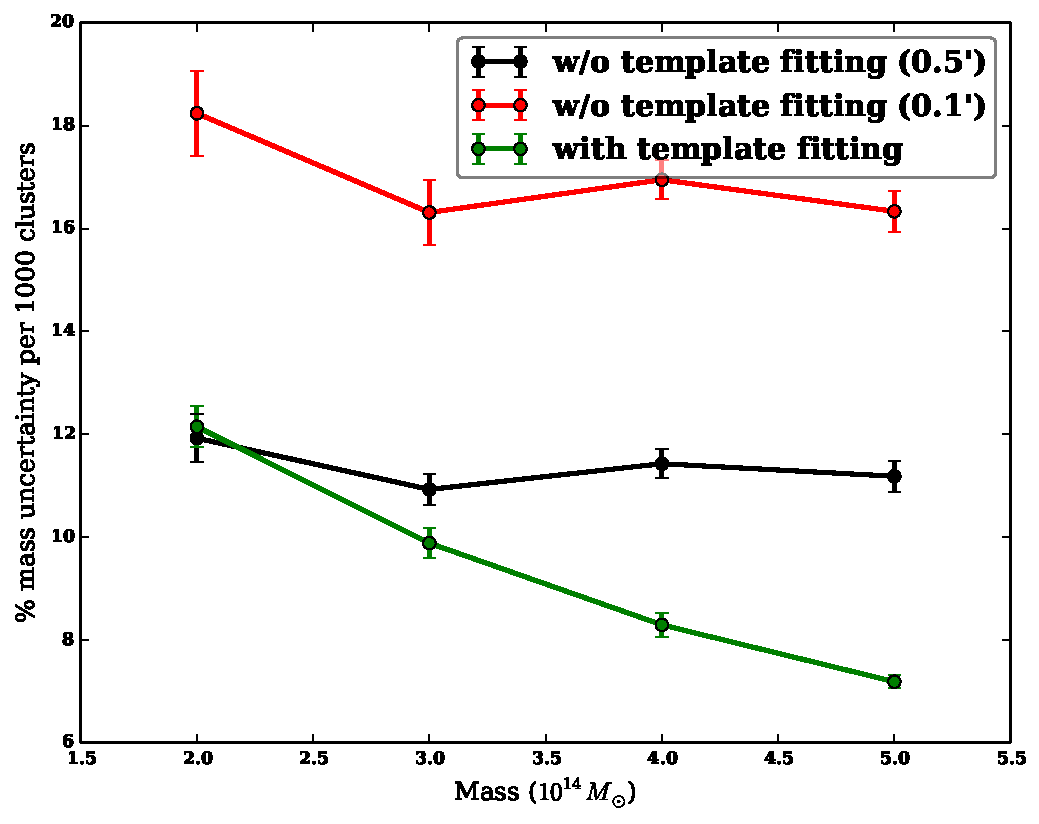
\includegraphics[width=\linewidth]{figs/miscentering_results.pdf}
 \caption{%Our new method is robust to realistic SZ simulations. 
The red and black solid curves show the performance of modified QE for the Sehgal and Takahashi simulations respectively. 
The dashed lines show the improvement in each case when template fitting is used to reduce the SZ variance in the small-scale map. 
 \sr{ Change xlabel to $\mvir$}.
 }
\label{fig:realistic_sims_pos}
\end{figure}
Previous works have found a positional offset of 0.5$\arcmin$ between the SZ and X-ray centroid \citep{linden14} or location of the brightest central galaxy (BCG)\citep{song12b}.
Template fitting methods provides optimal results if cluster center is the SZ center.
While this is not a problem for SZ selected clusters as both cluster and SZ center coincide, however, this may be a concern for clusters selected via X-ray or optical surveys.

In order to check the performance of our new method in the presence of miscentering, we draw draw an offset between the true and nominal cluster position from a normal distribution, $N(0, \sigma^{2})$. 
We add the \citet{arnaud10} SZ profile at the offset location.
We perform the template fitting approach with additional fitting parameters for positional offsets.
The results are shown in Fig. \ref{{fig:realistic_sims_pos}}.
We 
 for two normal distributions $\sigma = 0.1\am\$.
As shown in the Fig. \ref{{fig:realistic_sims_pos}} template fitting approach will substantially reduce the SZ variance even in the case of miscentering. 

%It is important to note that in such cases we can't use high pass filtered map as the lensing induced ``dipol'' present in the HPF map biases our fitting to lower masses. %as the fitted positional offset will be.
%This bias can be removed by combining different frequency channels to remove CMB with slight decrement in SNR.
%Detailed analysis of positional offset effects are out of the scope this p
}\fi

\subsection{Robustness of template fitting method}
\label{subsec:simsz}
\begin{figure}[ht]
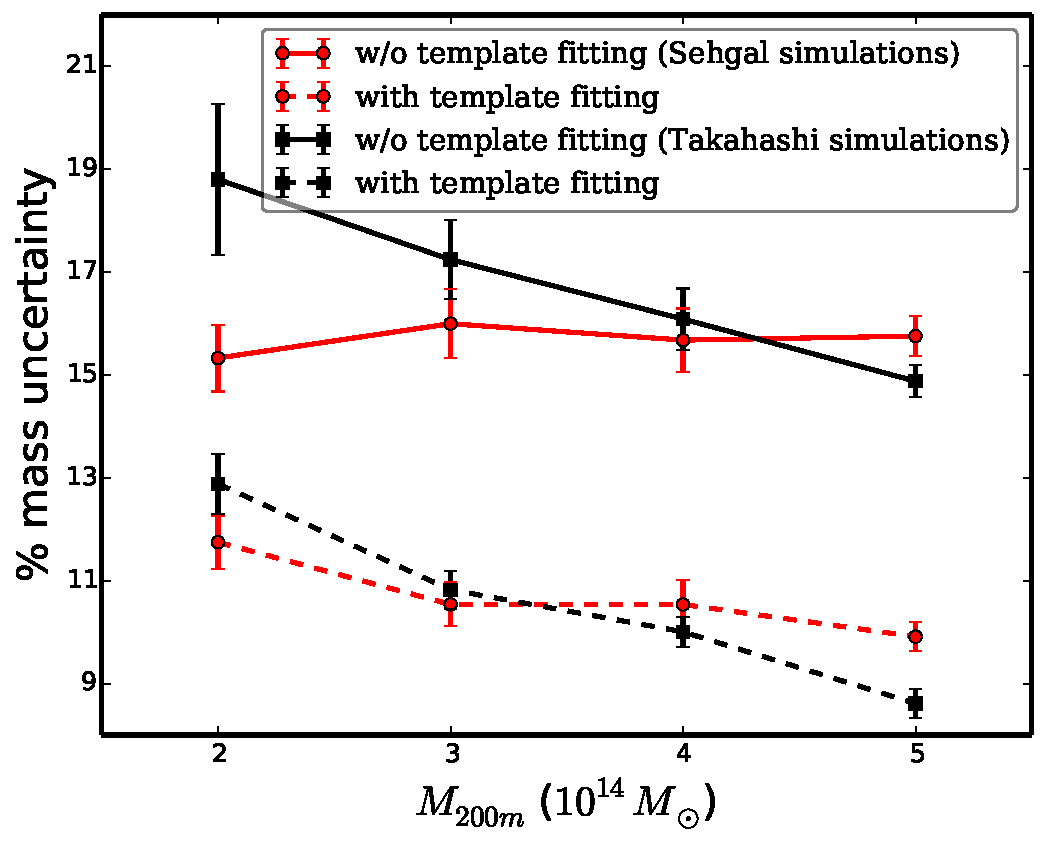
\includegraphics[width=\linewidth, keepaspectratio]{figs/Daisuke_Sehgal_results.pdf}
 \caption{
Our new method is robust to realistic SZ simulations. 
The red and black solid curves show the performance of modified QE for the Sehgal and Takahashi simulations respectively for a sample of 1000 clusters. 
The dashed lines show the improvement in each case when template fitting is used to reduce the SZ variance in the small-scale map. 
The plotted uncertainties are for a stack of 1000 galaxy clusters of the quoted mass at $z=0.7$. 
 }
\label{fig:realistic_sims}
\end{figure}
As shown in the last section, the refinement to the modified QE improves the fractional mass uncertainties significantly (above a mass threshold that depends on the survey noise) for the symmetric Arnaud profile. 
However, the question remains as to whether this improvement will continue with the more complex real SZ emission of galaxy clusters along with any other haloes along the line-of-sight.
To test this, we turn to the SZ simulations of \citet{sehgal10, takahashi17}. 
As noted in \S\ref{sec_tsz}, we draw SZ maps from these sims centered at the locations of similarly massed haloes. 
The results for these sims are shown in Fig.~\ref{fig:realistic_sims} for Gaussian template fitting. 
We have tested using both the Gaussian and Arnaud template fitting, and have found no appreciable difference. 
Red lines are for the Sehgal simulations and black lines for the Takahashi simulations. 
The solid lines are without template fitting, while the dashed lines show the improvement from template fitting in each case. 
 The apparent flattening of the red curve is due the limited number of higher mass clusters in the Sehgal simulation. 
 %Sehgal simulations are sample variance limited especially at higher masses.
 In this case of realistic SZ signals, however, we note that the performance is not equivalent to the idealized case presented as black solid curve in Fig. \ref{fig:template_fitting}. 
This is due to the residual SZ signals in the map coming from the template mismatch and from adjacent haloes which we do not attempt to remove.
 



%\subsection{Miscentering}
%Previous works have found a positional offset of 0.5$\arcmin$ between the SZ and X-ray centroid \citep{linden14} or location of the brightest central galaxy (BCG)\citep{song12b}.
%Template fitting methods provides optimal results if cluster center is the SZ center.
%While this is not a problem for SZ selected clusters as both cluster and SZ center coincide, however, this may be a concern for clusters selected via X-ray or optical surveys.
%In such cases our new method will be optimal if we have additional fitting parameters for positional offsets.
%It is important to note that in such cases we can't use high pass filtered map to fit template as the lensing induced ``dipole" present in the HPF map biases our fitting to lower masses. %as the fitted positional offset will be.
%This bias can be removed by combining different frequency channels to remove CMB with slight decrement in SNR.
%Detailed analysis of positional offset effects are out of the scope this p


\section{Forecasts}
\label{forecasts}

We now consider the impact of this method on the performance of upcoming CMB surveys, SPT-3G \citep{bender18}, SO \citep{so18} and CMB-S4 \citep{cmbs4-sb1}. 
For the latter two experiments, we only consider the large-aperture telescopes (LAT) with an experimental beam of $\theta_{\rm FWHM} = 1.^{\prime}4$ at 150 GHz and covering 40\% of the sky (see also Table \ref{table_forecast_setup}). 
For SPT-3G, we assume a survey area of 1500\,\sqdeg{} and an experimental beam of $\theta_{\rm FWHM} = 1.^{\prime}2$ at 150 GHz. 
We create a single cluster catalog realization for each experiment based on the noise levels at 150\,GHz. 
Note that for simplicity, we make no attempt to use frequency information to remove other temperature foreground signals such as the the CIB, nor to improve the noise level on the Compton-y map. 
These assumptions are likely to mean that the simulated cluster list is conservative since we are not taking advantage of the multiple frequency bands in each of these experiments. 

%The simulated 150\,GHz maps used for cluster finding include the primary CMB anisotropy, Gaussian foregrounds uncorrelated with the clusters, cluster SZ emission modelled using Arnaud profile, and the respective white noise levels as given in Table \ref{table_forecast_setup}.
%Next, we use the publicly available Halo Mass Function calculator \citep{murray13} to obtain the halo counts $d^{2}N/(dz\ d{\rm log}M$) per unit redshift ($\Delta z = 0.1$) and mass ($\Delta {\rm log} M = 14.05$) bin. %https://arxiv.org/abs/1306.6721
%Using the results from the above simulations, we get the number of clusters that will be detected above $\snr\ge 5$ by the three experiments. 
%This detection $\snr$ threshold should be conservative as well (the sample purity should be close to 1). 
%We estimate that SPT-3G, SO and CMB-S4 will detect respectively approximately 2,400, 27,000 and 75,000 clusters.


The three simulated cluster sample and assumed experimental parameters are passed through the cluster-lensing pipeline to estimate the mass uncertainty from CMB-cluster lensing on each stacked sample. 
 For forecasts we picks SZ profiles from \cite{takahashi17} simulations and as mentioned before we randomly pick all the halos which fall within 5\% of the desired mass and $\pm$0.2 of the desired redshift.
The results are given in Table \ref{table_forecast_setup}. 
We find that template fitting can reduce the percentage mass uncertainty for SPT-3G, SO and CMB-S4 by 28\%, 25\% and 30\% respectively.% 37\%, and 30\% for SPT-3G, SO, and CMB-S4 respectively. 
%The drop-off in the improvement for CMB-S4 here is because CMB-S4 is expected to detect lower mass clusters, where the SZ variance is less important relative to the CMB and instrumental noise variance. 
%When restricted to massive clusters at $M > 4 \times 10^{14}\msol$, we see an approximately 40\% improvement in detection significance for all three experiments. \tbd{confirm this}. 


\begin{table}
\caption{Forecasted mass uncertainties for SPT-3G, SO and CMB-S4  with the modified QE before and after removing the estimated SZ template.}
\footnotesize{
\centering
%\begin{tabular}{| C{1.5cm} | C{1.2cm}|  C{0.8cm} | C{1cm} | C{1cm} | C{1cm}  |}
\begin{tabular}{| c | c |  c | c | c  |}
\hline
% \multirow{2}{*}{Experiment} &  \multirow{2}{*}{$\Delta_{T}\ [\mu K^{\prime}]$} & \multirow{2}{*}{$f_{\rm sky}$} & \multirow{2}{*}{N$_{\rm clus}$} & \multicolumn{2}{c|}{$\Delta M/M$}\\
 \multirow{2}{*}{Exp.} &  \multirow{2}{*}{$\Delta_{T}\ [\mu K^{\prime}]$} & \multirow{3}{*}{N$_{\rm clus}$} & \multicolumn{2}{c|}{$\Delta M/M\ [\%]$}\\
\cline{4-5}
 & & & No template fitting & With template fitting\\\hline
SPT-3G & 2.2 & 2,400 &11.10& 8.00 \\\hline
 SO-LAT & 6.0 & 27,000 &2.82 &2.12 \\\hline
CMB-S4 & 1.73 & 75,000 &1.92 & 1.33\\\hline

\end{tabular}
}
\label{table_forecast_setup}
\end{table}


%%%%%%%%%%%%%%%%%%%%%%%%%%%%%%%%%%%%%%%%%%%%%
%%%%%%%%%%%%%%%%%%%%%%%%%%%%%%%%%%%%%%%%%%%%%
%%%%%%%%%%%%%%%%%%%%%%%%%%%%%%%%%%%%%%%%%%%%%
\section{Discussion and Conclusion}
\label{temp_fit_conclusions}

We have presented an improved version of the quadratic estimator (QE) to estimate galaxy cluster masses through CMB lensing. 
By projecting out an SZ template from the high-pass filtered leg of the QE, the algorithm substantially reduces the variance due to a cluster's own SZ emission. 
The SZ variance can be significant fraction of the total variance for high-mass clusters or low-noise surveys. 
Note that in the opposite limit of low masses or high noise (i.e. when the SZ variance is negligible), this template fitting may slightly reduce the overall S/N. 

%\sr{Keeping this paragraph depends on the sigma for SZ sims...}.
While the performance of the template fitting does depend on the fidelity with which the template accurately represents the true SZ signal, these variations do not seem to be a significant issue. 
In part this is because upcoming CMB experiments will not have sufficient angular resolution to resolve most of the structure in the SZ emission; the instrumental beam at 150\,GHz for a 6\,m telescope is slightly larger than a typical high-redshift cluster. 
%\sr{Check what happens to fig4: \sout{We get similar results as far as the final mass uncertainties for two independent sets of SZ simulations} %\citep{sehgal10, takahashi17}}. 
For mock SZ signals modeled using Arnaud profile, we find that the template removal approach reduces all of the additional variance due to the SZ signal. 
The improvement is not 100\% for realistic SZ signals \citep{sehgal10, takahashi17} because of the SZ emission from the adjacent haloes along the line-of-sight that we do not attempt to remove. 

The method presented in this work is not limited to the small-scale lensing. 
For example, \citet{madhavacheril18} demonstrated that the modified QE can also be employed to CMB lensing in general. 
However, as shown here the thermal SZ signal from clusters detected at high \snr{} adds extra variance in the reconstructed lensing maps. 
By using template fitting approach we reduced the variance significantly. 
In future CMB lensing work, we can use the template fitting approach instead of masking the massive galaxy clusters. 
%While the thermal SZ signal does not bias the lensing reconstruction, the extra variance introduces a bias in the lensing auto-spectrum. 
%Write more ....}

CMB-cluster lensing will be a key tool for galaxy cluster cosmology at high redshifts, while also providing a cross-check of optical weak lensing mass estimates at lower redshifts. 
%For future CMB surveys such as CMB-S4 and SO we can improve the mass uncertainty by 30\% and 37\% respectively.
For future surveys like CMB-S4 and Simons Observatory and for clusters above masses of $4\times 10^{14}\,\msol$, we find that template fitting yields a factor of 1.4 reduction in the mass uncertainties. 
These results will help us in the quest to understand dark energy and the accelerating expansion of the Universe.


\iffalse{
\subsection*{Acknowledgements}
We thank Eric Baxter, Federico Bianchini, Thomas Crawford, Nikhel Gupta, Daisuke Nagai, and W. L. Kimmy Wu for useful discussions regarding this project.

SP acknowledges support from MIPP, Laby Travel Bursary, and Melbourne International Engagement Award. 
SR acknowledges the support from NSF grants AST-1716965 and CSSI-1835865.
The work at Melbourne is supported by the Australian Research Council's Discovery Projects scheme (DP150103208).
We thank the high performance computation center at the University of Melbourne for providing access to the cluster \texttt{spartan.unimelb.edu.au}.
We acknowledge the use of \texttt{CAMB} \citep{lewis02b} and \texttt{HEALPIX} \citep{gorski05} routines. 
This research used resources of the National Energy Research Scientific Computing Center (NERSC), a DOE Office of Science User Facility supported by the Office of Science of the U.S. Department of Energy under Contract No. DE-AC02-05CH11231. 
 %This work is performed in the context of the South Pole Telescope scientific program. 
 %SPT is supported by the National Science Foundation through grant PLR-1248097.


\section{Results}
\subsection{Sources of uncertainty in the CMB-Cluster Lensing Measurement}
\begin{figure}[htb]
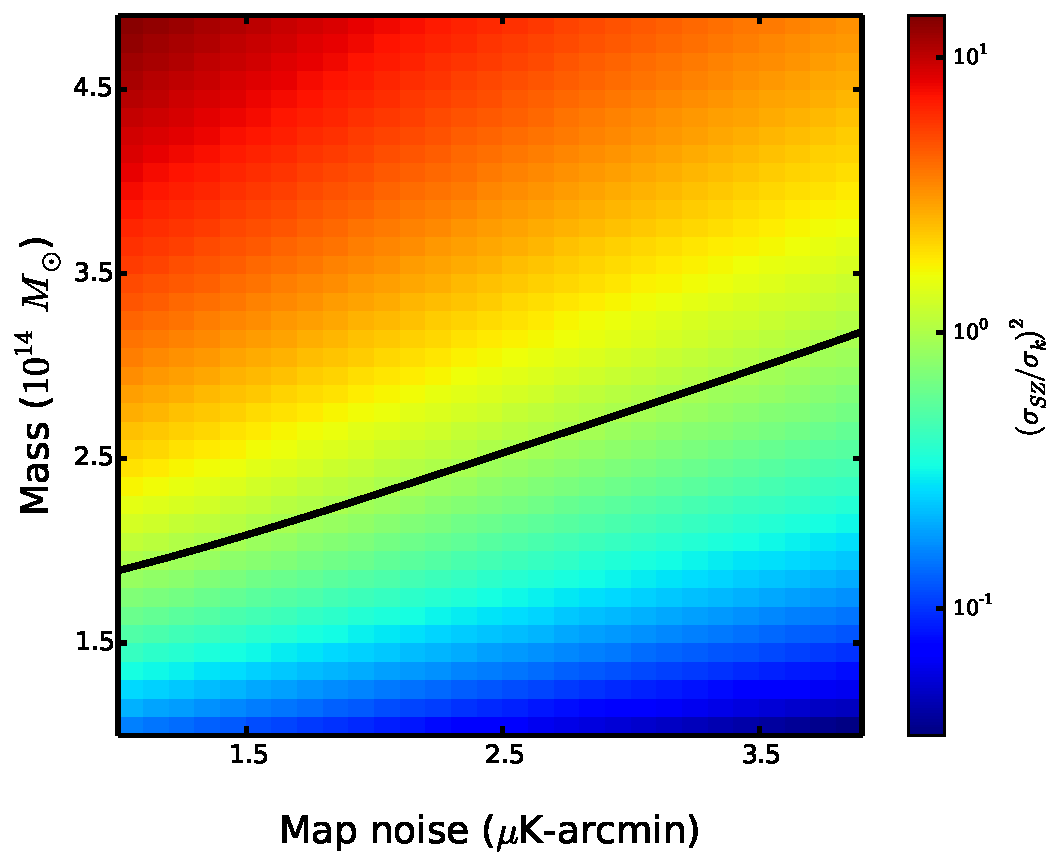
\includegraphics[width=\linewidth]{figs/contour_plot.pdf}
\vspace{-12pt}
 \caption{
 Ratio of SZ variance over kappa variance as a function of cluster mass and experimental noise level. 
 As expected the ratio increases with mass for a given experimental noise level. 
 The black solid line represents the points where the ratio SZ variance is equal to that of experimental noise.
 %\pending{(SR 20190130: Can you make a contour plot here to also include the effect of map depth? That will be more intuitive and one can easily figure out the mass threshold for which this method will be effective for different surveys.)\\}
 %\pending{Axis labels and caption disagree: sigma/variance} 
 %\pending{\textbf{Plot change: Keep the dashed line for 'SZ variance'. Add several horizontal lines at eg 1uk-arcmin, 3-uk-arcmin, 10uk-arcmin. Y-axis will no longer be the ratio}}
  }
 \label{fig:variance}
\end{figure}

Template fitting is intended to reduce the SZ variance, however it will do nothing for other sources of uncertainty such as instrumental noice, CMB sample variance and foreground emission (if not cleaned). 
Thus it will be useful to look at the relative magnitudes of these two terms, the SZ variance ($\sigma_{SZ}^{2}$) and the non-SZ variance ($\sigma_{\kappa}^{2}$), when interpreting the performance of template fitting in the next section.
The non-SZ variance, $\sigma_{\kappa}^{2}$, depends on the survey parameters (i.e.~instrumental noise, and the degree to which foregrounds are cleaned) but is independent of the cluster properties. 
We estimate $\sigma_{\kappa}^{2}$ following the approach in \citet{raghunathan18}. 
Briefly, we generate simulated CMB skies and add instrumental noise. 
We do not include the cluster's SZ emission or gravitational lensing signal since the goal is to estimate the other noise terms. 
We apply the lensing pipeline to the simulated skies to estimate the convergence maps. 
We fit the convergence map  to determine  a mass, and take the scatter in these inferred masses over 1000 simulations to be $\sigma_{\kappa}$. 
\tbd{think I've made this inaccurate. need to fix/explain better}

In contrast, the SZ variance should increase with cluster mass, $M$, roughly as $\sigma_{sz}^2 \propto M^{5/3}$, while being independent of the survey parameters. 
We estimate the SZ variance using the same suite as simulations, however now adding the cluster's SZ emission to the small-scale lensing map. 
We continue using an SZ-free map for other leg of the QE, the large-scale gradient map. 
As before, we estimate the convergence maps, fit for masses and take the scatter in these inferred masses to estimate $\sigma_{SZ}^{2}$ + $\sigma_{\kappa}^{2}$.

We present the ratio of the SZ to non-SZ variances, $\sigma_{SZ}^{2}$/$\sigma_{\kappa}^{2}$, as a function of survey noise level and cluster mass in Fig.\ref{fig:variance}.  
As expected, the ratio increases with mass at any given noise level. 
The black solid curve represents a ratio of unity when the SZ variance equals the non-SZ variance. 
We expect template fitting to significantly improve the mass uncertainties only for clusters above the black curve. 

\section{Results}
\label{sec_results}
%\pending{(SR 20190130: Have you tested the method for a slightly realistic tSZ profile like Sehgal?)} 

%In this section, first we quantify various sources of uncertanities in the final convergence maps as function of experimental noise level and cluster mass. 
%Later, we compare the performance of our new method for various templates. 
%We  then use some realistic SZ simulations to check the robustness of our method.
%Finally, we discuss the effects of miscentering on our lensing analysis.%three algorithms to estimate cluster masses:  
%(1) using an SZ-free map in the gradient leg and no SZ in the HPF leg of quadratic estimator 
%(2) using an SZ-free map only for the gradient leg of the QE, i.e. the modified QE, 
%and (3) improved version of the modified QE presented in this work, with an SZ-free map used for the gradient leg of the QE and projecting an SZ template out of the  HPF leg. 
%We rate the performance of each method,  as a function of both cluster mass and experimental noise levels,  by the estimated uncertainty on the recovered cluster mass. 

As shown in Fig.~\ref{fig:template_fitting}, we find that template fitting leads to a significant improvement in the final mass uncertainties for CMB-cluster lensing. 
For high-mass clusters, template fitting does nearly as well as in the idealized (non-physical) limit of having no SZ emission. 
In this figure, we are assuming an SPT-3G like experiment with FWHM=1$^\prime$ at 150\,GHz and a survey noise level of 3\,\ukarcmin{}. 
We compare four algorithms to estimate cluster masses.  
First, the red solid line shows the performance of the original modified QE without template fitting. 
This uses  an SZ-free gradient map 
(from a linear combination of 95 and 150\,GHz maps) and use a 150\,GHz map with SZ emission for the two legs of the QE. 
The second, black dotted line shows the results for an idealized case, where we again use an SZ-free gradient map but use a 150\,GHz map without SZ for the small-scale map. 
Obviously the latter assumption is unphysical since there will be SZ emission at 150\,GHz, but it shows the limit for how well perfect SZ subtraction might perform. 
Note that the relative performance improvement between the idealized and baseline cases increases with mass as expected. 
For these survey parameters, the idealized case has 17\% smaller uncertainties than the baseline for clusters of mass $1\times 10^14\,M_{\odot}$ and 50\% smaller for cluster masses of $5\times 10^14\,M_{\odot}$. 
Template fitting recovers nearly all of this gain for high-mass clusters. 


modified QE uncertainties 


(leaving out SZ)

for the gradient map and using 


no SZ in the small-scale map of the QE. 
(2) using an SZ-free map only for the gradient leg of the QE, i.e. the modified QE, 
 and (3) improved version of the modified QE presented in this work, with an SZ-free map used for the gradient leg of the QE and projecting an SZ template out of the  HPF leg.
 
 \subsection{Performance comparision} 
Here we compare three algorithms to estimate cluster masses:  
(1) using an SZ-free map in the gradient leg and no SZ in the HPF leg of quadratic estimator
(2) using an SZ-free map only for the gradient leg of the QE, i.e. the modified QE, 
 and (3) improved version of the modified QE presented in this work, with an SZ-free map used for the gradient leg of the QE and projecting an SZ template out of the  HPF leg. 


The performance of the three algorithms are shown in Fig. ~\ref{fig:template_fitting} as a function of cluster mass for an SPT-3G like experiment.
 All the curves show the percentage mass uncertanity for a sample 1000 clusters. 
Black curve represents an ideal case - SZ free gradient and no SZ in the second leg.
Though not realistic, it gives lower bound we can achieve with template fitting. 
On the other hand, red curve gives the upper bound with SZ-free gradient and Arnaud SZ profile in the second leg.
Blue and green curves show the improvement that can be achieved using our new method. 
For the blue and green curves, SZ signal present in the second leg is reduced by using Gaussian and Arnaud templates respectively.


As can be seen, both Arnaud and Gaussian template fitting perform equally well.
 This is unsurprising given that the angular size of the clusters is somewhat smaller than the instrumental beams; the beam-convolved signal is close to a Gaussian. 
While ideally template fitting approach should outperform modified QE at all mass scales, this is not the case in reality.
At low cluster masses, experimental noise level dominates over SZ noise.
 In such cases the template fitting would be poor and our new approach achieves a minimal improvement over modified QE. 
%At low cluster masses our new method is consistent with modified QE as experimental noise dominates. 
 On the other hand, at higher masses SZ variance is dominant source of uncertainty where the performance of our new method is considerable with the ideal case. %\sr{This definitely requires more explanation.} 
 \pending{The improvement which we obtain over the modified QE depends on the mass of the cluster and the experimental noise level.
 While ideally template fitting approach should outperform modified QE at mass scales, this is not the case in reality.}
 \begin{figure}[htb]
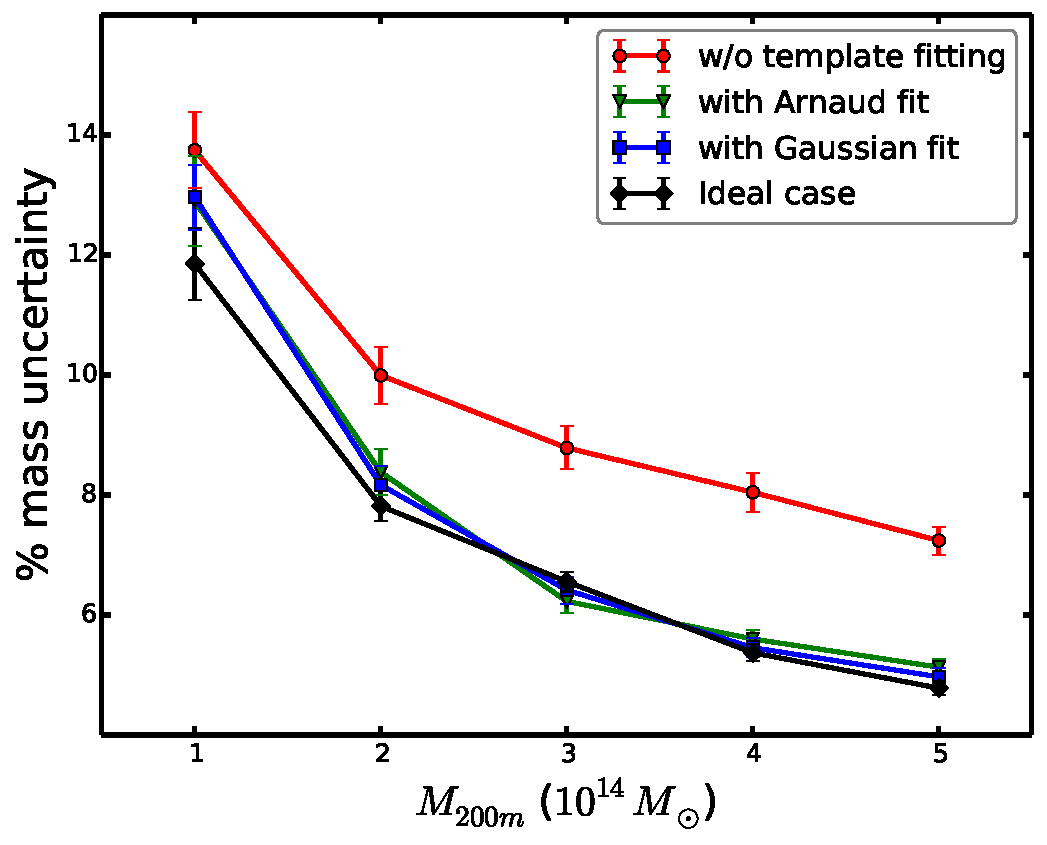
\includegraphics[width=\linewidth]{figs/uncen_vs_mass.pdf}
 \caption{
 Projecting out an SZ template from the second leg o the modified QE improves the performance for all masses considered. 
 Here we show the percentage mass uncertainties from three methods for a sample of 1000 clusters at a experimental noise level of 3\,\ukarcmin{}.
 All the curves use an SZ-free map for the gradient, but make different assumptions about the second, high-pass filtered map. 
 %In the ideal case (red), the HPF map assumes 150\,GHz map noise levels with zero SZ signal -- a physically unrealistic option that is included to show the lower bound to how well a method to deal with the SZ signal might perform. 
 %At the other extreme, the green curve shows the results when a raw 150\,GHz map is used for the HPF leg, i.e.~it includes the full effects of SZ variance and sets the upper bound on the performance of methods to remove the SZ variance. 
 %The uncertainties for the simple template fitting method are shown by the black line. 
 %As expected, it falls between the two extremes. 
 %For low-mass clusters \pending{(M = 2e14) }, the template fitting method only marginally improves the results -- reducing the already small SZ variance is balanced against the information loss from the mode projection. 
%At higher masses where the SZ variance is dominant since it scales as $M^{5/3}$, the template fitting method does extremely well compared to using an 150\,GHz map (the green curve). 
 \sr{Replace ``mQE' to w/o template fitting. They are all mQE. Change xlabel to $\mvir$. Change line styles to match text}.
 }
\label{fig:template_fitting}
\end{figure}
\subsection{Robustness of template fitting method}
\label{subsec:simsz}
As seen in the Fig.~\ref{fig:template_fitting} our refinement for modified QE improves the fractional mass uncertanties sginificantly for all the masses considered.
 However, the realistic SZ may not be a radially symmetric as Arnaud profile predicts.
So, in order to check the robustness of our new method we used realistic SZ simulations from Sehgal et al \cite{sehgal10} and Takahashi et al \cite{takahashi17}, the results of which are show in Fig.~\ref{fig:realistic_sims}. 
We have only considered Gaussian fitting for the realistic simulations as there is no difference in the performance of both templates.  
The red and black curves in the figure are the results of modified QE for Sehgal and Daisuke sims and the corresponding dashed curves show the improvements we obtain after subtracting Gaussian template from the second leg of modified QE.
 The apparent flattening of the red curve is due the limited sample variance of Sehgal simulation at higher masses.
 %Sehgal simulations are sample variance limited especially at higher masses.

\begin{figure}[htb]
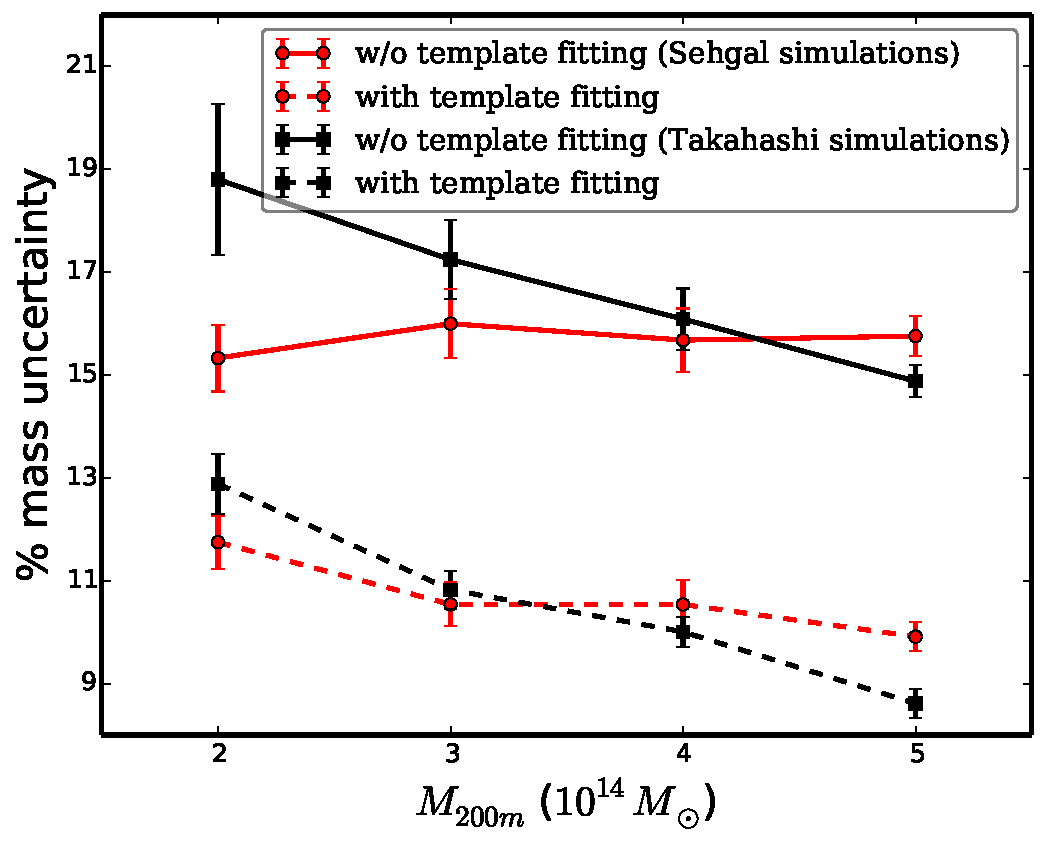
\includegraphics[width=\linewidth]{figs/Daisuke_Sehgal_results.pdf}
 \caption{
Our new method is robust to realistic SZ simulations. 
The red and black solid curves show the performance of modified QE for the Sehgal and Takahashi simulations respectively. 
The dashed lines show the improvement in each case when template fitting is used to reduce the SZ variance in the small-scale map. 
 \sr{ Change xlabel to $\mvir$}.
 }
\label{fig:realistic_sims}
\end{figure}

\subsection{Miscentering}
Previous works have found a positional offset of 0.5$\arcmin$ between the SZ and X-ray centroid \citep{linden14} or location of the brightest central galaxy (BCG)\citep{song12b}.
Template fitting methods provides optimal results if cluster center is the SZ center.
While this is not a problem for SZ selected clusters as both cluster and SZ center coincide, however, this may be a concern for clusters selected via X-ray or optical surveys.
In such cases our new method will be optimal if we have additional fitting parameters for positional offsets.
It is important to note that in such cases we can't use high pass filtered map as the lensing induced ``dipole" present in the HPF map biases our fitting to lower masses. %as the fitted positional offset will be.
This bias can be removed by combining different frequency channels to remove CMB with slight decrement in SNR.
%Detailed analysis of positional offset effects are out of the scope this p
\begin{figure}[htb]
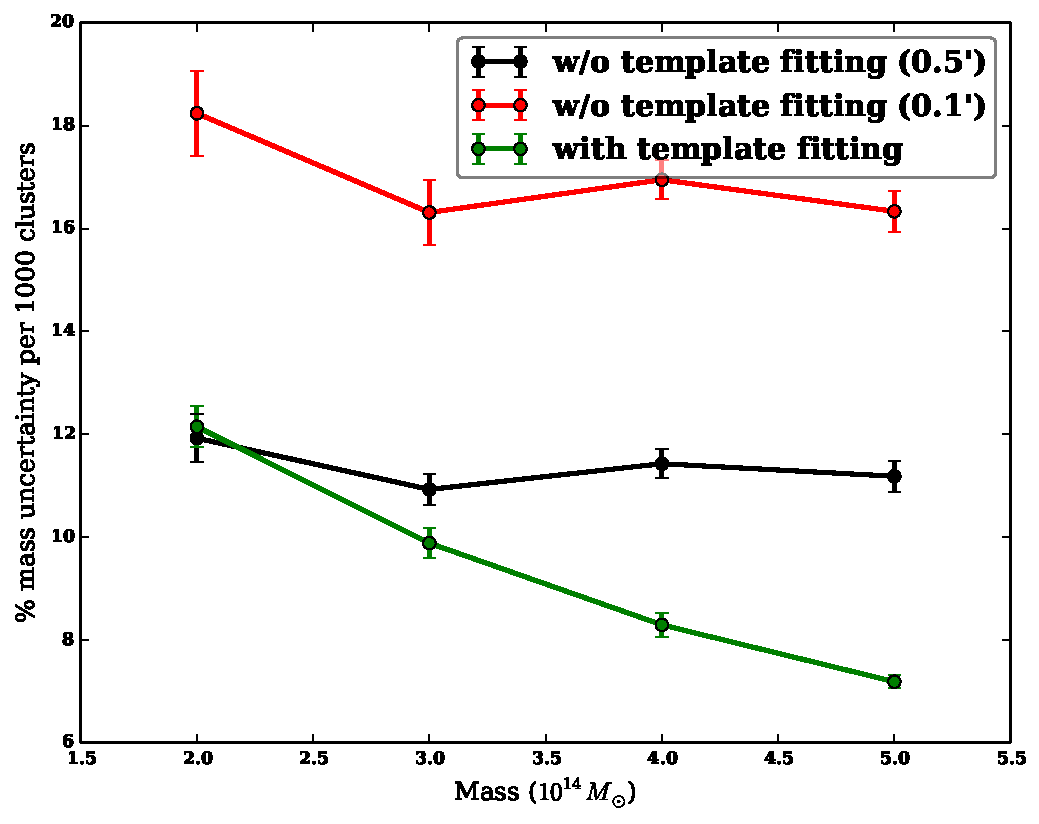
\includegraphics[width=\linewidth]{figs/miscentering_results.pdf}
 \caption{
Our new method is robust to realistic SZ simulations. 
The red and black solid curves show the performance of modified QE for the Sehgal and Takahashi simulations respectively. 
The dashed lines show the improvement in each case when template fitting is used to reduce the SZ variance in the small-scale map. 
 \sr{ Change xlabel to $\mvir$}.
 }
\label{fig:realistic_sims}
\end{figure}

\section{Forecasts}
\label{forecasts}
Now we predict the uncertainties expected on the stacked mass for the cluster samples from the CMB-S4 \citep{cmbs4-sb1} and the Simons Observatory (SO)\footnote{\sr{SO Goal: write more}} \citep{SO18} experiments. 
In both cases, we only consider the large-aperture telescopes (LAT) with an experimental beam of $\theta_{\rm FWHM} = 1.^{\prime}4$ at 150 GHz and covering 40\% of the sky (see also Table \ref{table_forecast_setup}).
We generated the expected cluster samples for the experiments without any foreground reduction technique using the 150 GHz channel. 
For this, using simulations we first estimate the detection significance \snr{} for clusters as a function of mass and redshift for the two experiments. 
The simulations contain signals from the primordial CMB, Gaussian foregrounds uncorrelated with the cluster, cluster tSZ emission modelled using Arnaud profile, and the respective white noise levels as given in Table \ref{table_forecast_setup}.
The Gaussian foregrounds components were added using the measurements made by the SPT-SZ experiment \citep{george15} and contain emissions from radio, dusty galaxies, and the SZ signals from the low mass haloes that were unresolved by the SPT-SZ experiment. 
Next, we use the publicly available Halo Mass Function calculator \citep{murray13} to obtain the halo counts ($dN/dz/d{\rm log}M$) per unit redshift ($\Delta z = 0.1$) and mass ($\Delta M = xx$) bin. %https://arxiv.org/abs/1306.6721
Using the SNR look-up table from the above simulations, we get the number of clusters that will be detected above \snr$\ge 5$ by both the experiments. 
We estimate that CMB-S4 (SO) will detect approximately 75,000 (27,000) clusters.
More details about the software used tp generate the cluster sample will be given in a future work.
We feed these cluster samples into our lensing pipeline and predict the uncertainty in the stacked mass for the two samples. 
The results are given in Table \ref{table_forecast_setup}. 
\pending{ We find  ... w/o tSZ removal and xx after tSZ removal ..}
 \pending{bit about SO and S4 including configuration and improvements obtained }

\
}\fi





\iffalse{
\subsection{Modifying the Quadratic Estimator to remove SZ bias}
\label{sec_mQE}


Gravitational lensing by a compact object like a galaxy cluster creates a small-scale dipole pattern in the direction of the large-scale CMB temperature gradient. 
The QE \citep{hu02a} is based on extracting the correlation between dipole and the background gradient to estimate the lensing convergence $\hat{\kappa}_{\bL}$. 
Specifically, the lensing convergence can be estimated from a weighted product of filtered versions of a gradient map $G(\hat{n})$ and  small-scale lensing map $L(\hat{n})$: 
\begin{equation}
\hat{\kappa}_{\bL} = -A_{\ell} \int d^{2}\bnhat\ e^{-i\bnhat\cdot\bL}\ {\rm Re} \left\{ \nabla \cdot \left[ G(\bnhat) L^{*}(\bnhat)\right]\right\}.
\label{eq_QE_kappa}
\end{equation} 
Here, $\bnhat$ is the pointing unit vector, $\bL$ is angular multipole, and $A_{l}$ is a normalization factor. 


While designed to pull out the lensing-induced correlations between large-scale and small-scale CMB anisotropy, the QE is also sensitive to  correlations due to foreground emission.
Of particular concern is  the cluster's own SZ emission, which is typically an order of magnitude larger than lensing signal. 
As shown by \citet{hu07}, the magnitude of the SZ bias can be lowered by decreasing the characteristic scale of the low pass filter on the gradient map. 
However, a stronger low-pass filter obviously reduces the number of modes used to measure the gradient, and thus decreases the signal-to-noise. 
The modified QE instead eliminates this bias by using an SZ-cleaned map for the large-scale gradient map. 
The large-scale gradient map is chosen because the CMB has much more power on large scales, so the noise penalty from SZ removal has minimal impact. 
Note that while multiple foregrounds can be removed in principle, in practice the focus has been on removing the SZ signal. 
This is simply because the SZ signal introduces the largest bias.  
With the SZ signal present in only one of the two maps, there is no SZ-induced correlation between the two maps and no net bias on the reconstruction of the lensing convergence. 
}\fi




\iffalse{
However the SZ emission in the small scale lensing map does add noise to the lensing reconstruction. 
Since under self-similarity the SZ flux, $y$, is expected to scale with  \mbox{cluster mass $M$} as $y \propto M^{5/3}$ while the lensing signal is linear in mass, the additional SZ variance will generally be more important for high-mass clusters. 
The SZ variance will also be more important in low-noise surveys, i.e.~when it is larger than the instrumental noise in the convergence map.%the nominal variance of convergence map set by the instrumental noise level of the experiment.  Cosmic Microwave Background (CMB) has no power at galaxy cluster angular scales due to silk damping and hence can be approximated as a gradient on arc minute scales.
 Gravitational lensing of CMB by cluster induces a dipole kind of structure on the top of gradient.
 The correlation between the background gradient and lensing dipole is known as gradient approximation.    
The QE \citep{hu02a} exploits the gradient approximation to estimate the lensing convergence profile $\hat{\kappa}$. 
 Gradient approximation doesn't hold for all Fourier modes, in fact it holds good for only those Fourier modes which are correlated by reconstruction. 
 Specifically, the lensing convergence can be estimated from a weighted product of filtered versions of a gradient map $G(\hat{n})$ and  small-scale lensing map $L(\hat{n})$: 
\begin{equation}
\hat{\kappa}_{\bL} =-A_{\ell}\int d^{2}\bnhat\ e^{-i\bnhat\cdot\bL}\ {\rm Re} \left\{ \nabla \cdot \left[ G(\bnhat) L^{*}(\bnhat)\right]\right\}.
\label{eq_QE_kappa}
\end{equation} 
Here, $\bnhat$ is the pointing unit vector, $\bL$ is angular multipole, and $A_{l}$ is a normalization factor. 

While designed to pull out the lensing-induced correlations between large-scale and small-scale CMB anisotropy, the QE is also sensitive to  correlations due to foreground emission.
Of particular concern is  the cluster's own SZ emission, which is typically an order of magnitude larger than lensing signal. 
Two ways have been discussed in literature to eliminate/reduce the SZ bias.
One way is to exploit the multiple frequency dependence of SZ signal and use linear combination of different frequencies to remove SZ.
While this method completes eliminates SZ bias, it significantly increases the statistical uncertainty due to the higher noise level of the combined map.
Another way is to lower the characteristic scale of the low pass filter on the gradient map as shown in  \citet{hu07}.
Lowering the gradient cut results in separation of the modes present in gradient and small scale dipole map; hence reducing the unwanted correlation. 
However, a stronger low-pass filter obviously reduces the number of modes used to measure the gradient, and thus decreases the signal-to-noise. 

On the other hand, the modified QE instead eliminates this bias without increasing the variance significantly by using an SZ-cleaned map for the large-scale gradient map. 
The large-scale gradient map is chosen because the CMB has much more power on large scales, so the noise penalty from SZ removal has minimal impact. 
Note that while multiple foregrounds can be removed in principle, in practice the focus has been on removing the SZ signal. 
This is simply because the SZ signal introduces the largest bias.  
With the SZ signal present in only one of the two maps, there is no SZ-induced correlation between the two maps and no net bias on the reconstruction of the lensing convergence. 

However the SZ emission in the small scale lensing map does add noise to the lensing reconstruction. 
Since under self-similarity of the SZ flux, $y$, is expected to scale with cluster mass $M$ as $y\propto M^{5/3}$ while the lensing signal is linear in mass, the additional SZ variance will generally be more important for high-mass clusters. 
The SZ variance will also be more important in low-noise surveys, i.e.~when it is larger than the instrumental noise in the convergence map.%the nominal variance of convergence map set by the instrumental noise level of the experiment. 

\subsection{Template fitting to reduce the SZ variance}
\label{sec_sz_template_fitting}

As mentioned earlier, an obvious way to eliminate this SZ variance is by using SZ-free maps for both the small-scale and gradient maps. 
Of course this would undo the advantages of the modified QE for the instrumental noise in the small scale map. 
One can also reduce this extra variance by projecting out a model template for the SZ signal, and thereby reducing the total amount of SZ power in the small-scale map. 

Template fitting has been considered previously in the context of the original QE \citep{tbd?}. 
However, in that setting, residual SZ signals would bias the lensing masses. 
%\tbd{the next needs a citation/details on what size cluster} 
 Even one percent of residual SZ signal would lead to bias of six percent in mass estimation. 
This is not a problem in modified QE with SZ-free gradient map the residual SZ in the second leg won't introduce any bias. %within certain limits, template fitting and any residuals will not bias the modified QE.

To be unbiased, the template must not couple (on average) to the  CMB lensing signal. 
This can be achieved by either fitting the template to a Compton  y-map (i.e. using the different spectral dependence of the SZ and CMB to eliminate the CMB), or by using a template that has no average correlation with the lensing dipole pattern. 
The latter can be achieved by a radially symmetric template, fixed at the cluster position.
To illustrate this we constructed a plane temperature gradient field and lensed it with galaxy cluster of mass $M_{200m} = 5*10^{14}M_{\odot}$. 
We fit a radially symmetric Gaussian profile to the lensing dipole signal as shown in Fig. ~\ref{fig:no_bias}. 
 The left panel in Fig. ~\ref{fig:no_bias} is the lensing dipole signal and right panel is the best fit Gaussian profile. 
 As can be seen the amplitude of the resultant Gaussian fit is of the order of $10^{-15}$.

\begin{figure}
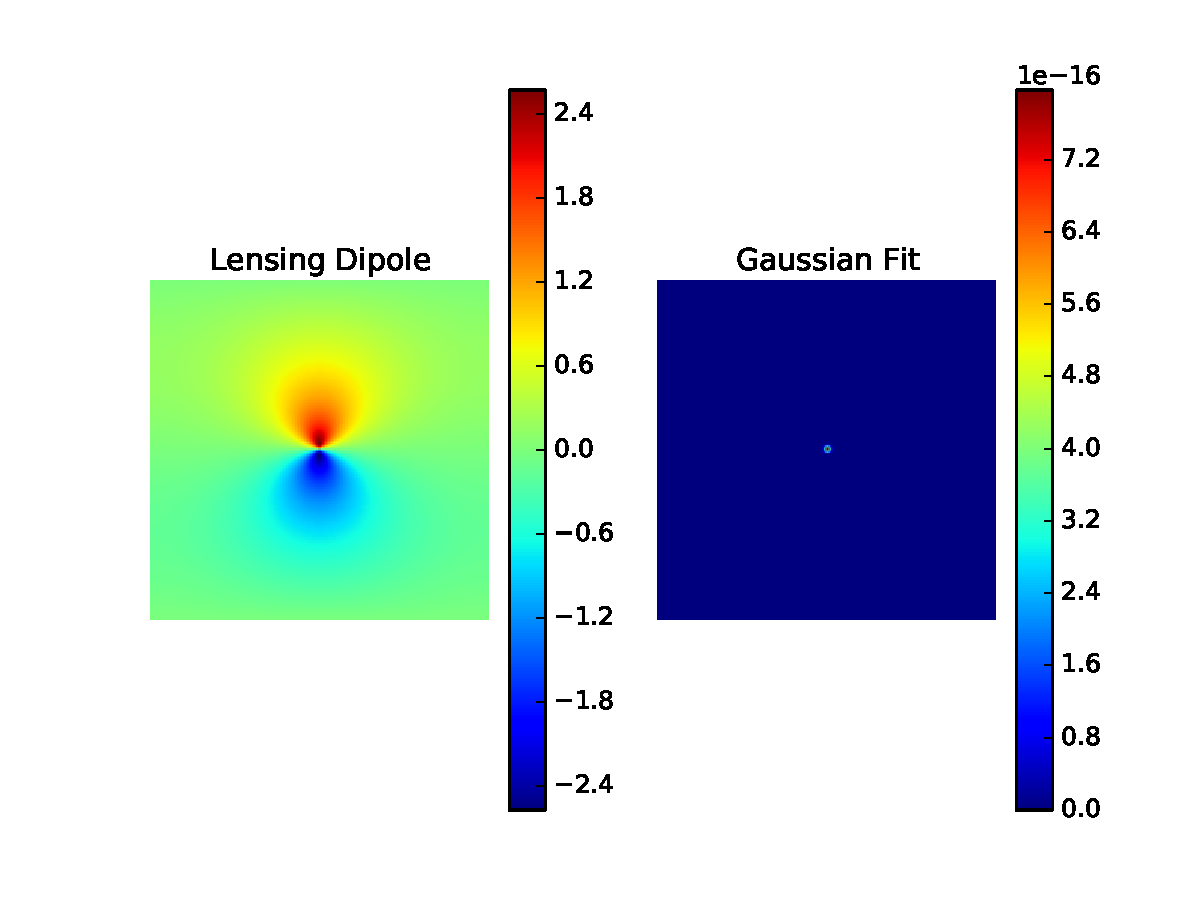
\includegraphics[width=\linewidth]{figs/template_fitting_bias.pdf}
 \caption{\pending{explain why no bias}
 } 
\label{fig:no_bias}
\end{figure}

If the position is freed, the template can shift to pick up the negative lobe of the lensing dipole signal resulting in a low bias. 
Given the impossibility in creating a `perfect' SZ template, the template fitting will not completely eliminate the SZ signal in the small-scale map. 
However, template fitting can significantly reduce the SZ power in the small-scale map, and thus reduce the SZ noise penalty on the lensing mass reconstruction. 

In this work, we take the tact of fitting a radially symmetric template at the fixed cluster location. 
Unless otherwise noted, we assume the beam to be a Gaussian with FWHM = 1\arcmin{} at 150 GHz and 1\arcmin.7 at 90\,GHz. 
As this beam size is significant compared to the actual size of clusters at $z>0.3$, clusters are approaching the effective point source limit where the specific details of their shape would not matter. 
Thus we choose to use a simple Gaussian template as the baseline template in this work. 
We also compare the results to template fitting with more physically motivated Arnaud profile \citep{arnaud10}, convolved by the experimental Gaussian beam.  
The residuals of removing a 2\arcmin.0 FWHM Gaussian from an Arnaud profile convolved by a 1\arcmin.7 beam are illustrated in Fig.~\ref{fig:residual}. 
As argued above, the Gaussian significantly reduces the SZ signal despite the mismatch between the assumed profile and input SZ model. 
While there should be small variations in the typical size of the cluster's SZ emission with mass and redshift, we neglect these variations and fix the size of the templates based on the expected median mass and redshift of the sample.

Since the template will be applied to that small-scale map that has been high pass filtered at $\ell > 2000$, we apply a matching high pass filter to the map used for fitting and the SZ model template. 
This high-pass filter step is done in cutouts of $100\arcmin \times 100\arcmin$; we then pull out a central $10\arcmin \times 10\arcmin$ cutout at the cluster location for fitting the template. 
Since both the SZ emission and lensing signal extraction is concentrated within a few arcminutes of the cluster center, there is little reason to fit over a larger area. 
We allow for two free parameters in the fitting: the overall amplitude of the template, and a constant DC offset. 
Note that given the high-pass filter, we expect (and find) the DC term to be effectively zero. 
In any case, while we fit for a DC term when normalizing the template, we do not then remove the DC term. 
Only the template is subtracted from the small-scale map.

With template fitting included, the Fourier transforms of the two maps used by the quadratic estimator can be written down as:
\begin{eqnarray}
G_{\ell} &=& i\ell W^{G}_{\ell} T^{\rm SZ-free}_{\ell}\\
L_{\ell} &=& W^{L}_{\ell} \left(T_{\ell} - T_\ell^{\rm SZ-template}\right)
\end{eqnarray}
where, $G_{\ell}$ is the large-scale gradient map and $L_{\ell}$ is the small-scale map. 
$W^{G}_{l}$ and $W^{L}_{l} $ are the Wiener filters to maximize the lensing signal \cite{hu06}. 
The mm-wave map is $T_{\ell}$ while the constructed SZ-free map is $T^{\rm SZ-free}_{\ell}$. 
Compared to the modified QE \citep{madhavacheril15,raghunathan18}, the new element is the $T_\ell^{\rm SZ-template}$ term representing the SZ template fit. 

\begin{figure}
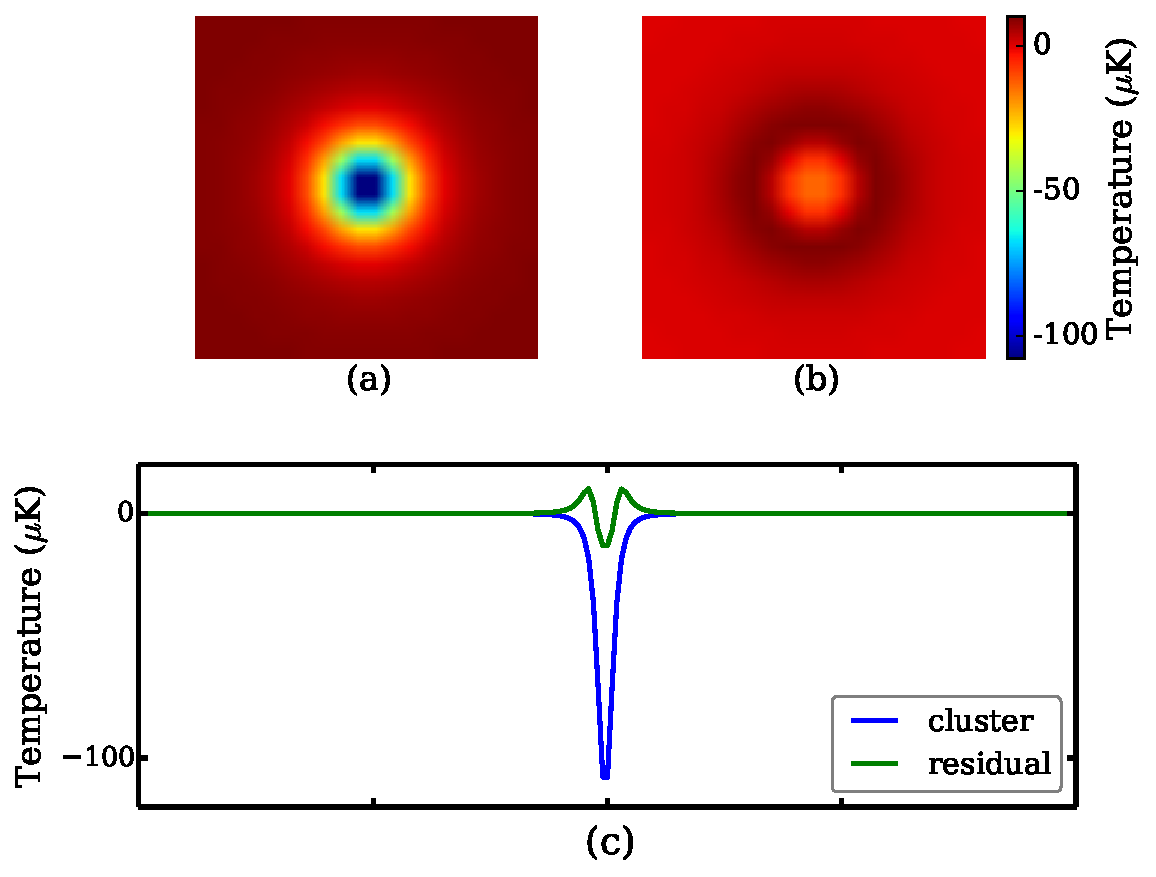
\includegraphics[width=\linewidth]{figs/template_fitting.pdf}
 \caption{Template fitting significantly reduces SZ power, even with an imperfect match between the template and true SZ signal. 
The top left panel (a) shows the expected Arnaud profile for a galaxy cluster of mass $\mvir = 5 \munits$ at z=0.7 after being smoothed by Gaussian beam with FWHM= 1\arcmin.7.
The top right panel (b) shows the residuals after subtracting the best-fit 2\arcmin.0 FWHM Gaussian (the amplitude is free, but the FWHM is fixed). 
The lower panel (c) shows one-dimensional slices through each panel: the solid, blue line is a slice through the beam-convolved Arnaud profile of (a), and the dashed green line is a slice through the residual map in (b). 
 } 
\label{fig:residual}
\end{figure}
}\fi
\small
\setlength{\bibsep}{1.0mm}
%\bibliographystyle{avebib}
%\bibliographystyle{plainnat}
\bibliographystyle{mn2e}
\bibliography{bibliography}
\normalsize

\appendix%
    \chapter{Appendix A}
\section{Section in an appendix}

This is an appendix chapter.

\end{document}

